% =====================================================================
%  Optimizacijske metode u razvoju i upravljanju sustava
%  Skripta za ucenje, sastavljena iz predavanja 01-08 i vjezbi 1-5
%  Format: A4, za ispis
% =====================================================================
\documentclass[11pt,a4paper,oneside]{report}

% =====================================================================
%  Preambula skripte -- A4, za ispis
% =====================================================================

\usepackage[T1]{fontenc}
\usepackage{lmodern}
\usepackage{polyglossia}
\setdefaultlanguage{croatian}
\setotherlanguage{english}

\usepackage{amsmath,amssymb,amsthm}
\usepackage{mathtools}
\usepackage{microtype}

\usepackage[
  a4paper,
  top=2.4cm, bottom=2.4cm, left=2.6cm, right=2.6cm,
  headheight=14pt, footskip=1.1cm
]{geometry}

\usepackage{graphicx}
\graphicspath{{figures/}{../figures/}}
\usepackage{float}
\usepackage{booktabs}
\usepackage{array}
% stupac fiksne sirine s ravnom lijevom marginom (bez rastegnutih razmaka)
\newcolumntype{P}[1]{>{\raggedright\arraybackslash}p{#1}}
\usepackage{longtable}
\usepackage{enumitem}
\usepackage{xcolor}
\usepackage[most]{tcolorbox}
\usepackage{fancyhdr}
\usepackage{titlesec}
\usepackage{caption}

\usepackage[hidelinks]{hyperref}
\hypersetup{
  pdftitle={Optimizacijske metode u razvoju i upravljanju sustava --- skripta},
  pdfauthor={Skripta sastavljena iz predavanja i vjezbi},
  bookmarksnumbered=true
}

% --------------------------------------------------------------- boje
\definecolor{fsbcrvena}{HTML}{9B1B30}
\definecolor{tamnoplava}{HTML}{1F3864}
\definecolor{svijetlosiva}{HTML}{F2F2F2}
\definecolor{zelena}{HTML}{1E6B3A}
\definecolor{narancasta}{HTML}{B35C00}

% ------------------------------------------------------- naslovi
\titleformat{\chapter}[display]
  {\normalfont\huge\bfseries\color{fsbcrvena}}
  {\Large\MakeUppercase{\chaptertitlename} \thechapter}{10pt}{\Huge}
\titlespacing*{\chapter}{0pt}{-20pt}{28pt}

\titleformat{\section}
  {\normalfont\Large\bfseries\color{tamnoplava}}{\thesection}{0.7em}{}
\titleformat{\subsection}
  {\normalfont\large\bfseries\color{tamnoplava}}{\thesubsection}{0.7em}{}
\titleformat{\subsubsection}
  {\normalfont\normalsize\bfseries}{\thesubsubsection}{0.7em}{}

\setcounter{secnumdepth}{3}
\setcounter{tocdepth}{2}

% ------------------------------------------------------- zaglavlje
\pagestyle{fancy}
\fancyhf{}
\fancyhead[L]{\small\nouppercase{\leftmark}}
\fancyhead[R]{\small\thepage}
\renewcommand{\headrulewidth}{0.4pt}
\fancypagestyle{plain}{\fancyhf{}\fancyfoot[C]{\small\thepage}%
  \renewcommand{\headrulewidth}{0pt}}

% ------------------------------------------------------- razmaci
\setlength{\parindent}{0pt}
\setlength{\parskip}{0.55em}
\renewcommand{\arraystretch}{1.15}
\setlist{itemsep=0.25em, topsep=0.35em, parsep=0pt}

% =====================================================================
%  Okviri za tipove sadrzaja
% =====================================================================

\newtcolorbox[auto counter, number within=chapter]{definicija}[1][]{%
  enhanced, breakable, colback=svijetlosiva, colframe=tamnoplava,
  boxrule=0.9pt, arc=2pt, left=8pt, right=8pt, top=6pt, bottom=6pt,
  fonttitle=\bfseries\color{white},
  title={Definicija~\thetcbcounter\ifstrempty{#1}{}{: #1}}}

\newtcolorbox[auto counter, number within=chapter]{teorem}[1][]{%
  enhanced, breakable, colback=white, colframe=fsbcrvena,
  boxrule=0.9pt, arc=2pt, left=8pt, right=8pt, top=6pt, bottom=6pt,
  fonttitle=\bfseries\color{white},
  title={Teorem~\thetcbcounter\ifstrempty{#1}{}{: #1}}}

\newtcolorbox[auto counter, number within=chapter]{zadatak}[1][]{%
  enhanced, breakable, colback=white, colframe=zelena,
  boxrule=1.1pt, arc=2pt, left=8pt, right=8pt, top=6pt, bottom=6pt,
  fonttitle=\bfseries\color{white},
  title={Zadatak~\thetcbcounter\ifstrempty{#1}{}{ --- #1}}}

\newtcolorbox{napomena}[1][]{%
  enhanced, breakable, colback=white, colframe=narancasta,
  boxrule=0.6pt, arc=2pt, left=8pt, right=8pt, top=5pt, bottom=5pt,
  borderline west={2.5pt}{0pt}{narancasta},
  fonttitle=\bfseries\color{white},
  title={Napomena\ifstrempty{#1}{}{: #1}}}

\newtcolorbox{izvor}[1][]{%
  enhanced, breakable, colback=svijetlosiva, colframe=svijetlosiva,
  boxrule=0pt, arc=1pt, left=8pt, right=8pt, top=5pt, bottom=5pt,
  borderline west={2.5pt}{0pt}{tamnoplava}}

% okvir za upute za rucno crtanje grafa
\newtcolorbox{crtanje}[1][]{%
  enhanced, breakable, colback=white, colframe=tamnoplava,
  boxrule=0.6pt, arc=2pt, left=8pt, right=8pt, top=6pt, bottom=6pt,
  fonttitle=\bfseries\color{white},
  title={Kako to nacrtati rukom\ifstrempty{#1}{}{: #1}}}

% =====================================================================
%  Kratice za matematiku
% =====================================================================
\newcommand{\R}{\mathbb{R}}
\newcommand{\Feas}{\mathcal{F}}
\newcommand{\T}{^{\top}}
\newcommand{\opt}{^{\star}}
\DeclareMathOperator*{\argmin}{arg\,min}
\DeclareMathOperator*{\argmax}{arg\,max}
\DeclareMathOperator{\dom}{dom}
\DeclareMathOperator{\tr}{tr}
\DeclareMathOperator{\rank}{rank}
\DeclareMathOperator{\diag}{diag}
\DeclareMathOperator{\sgn}{sgn}
\DeclareMathOperator{\dist}{dist}
\newcommand{\dd}{\mathrm{d}}
\newcommand{\uzogr}{\text{uz ograničenja}\quad}
\newcommand{\minim}{\text{minimiziraj}\quad}

% oznaka izvorne stranice u slajdovima
\newcommand{\str}[1]{\textcolor{gray}{\footnotesize[str.~#1]}}


\begin{document}

% ------------------------------------------------------- naslovnica
\begin{titlepage}
\centering
\vspace*{2.5cm}

{\Huge\bfseries\color{fsbcrvena} Optimizacijske metode\\[0.3cm]
u razvoju i upravljanju sustava\par}

\vspace{1.2cm}
{\LARGE\bfseries Skripta za učenje\par}

\vspace{0.6cm}
{\large Cjelovita obrada gradiva --- od nule do ispita\par}

\vspace{2.5cm}
\rule{0.75\textwidth}{0.8pt}

\vspace{0.8cm}
\begin{minipage}{0.8\textwidth}
\centering\large
Skripta je sastavljena \textbf{isključivo} iz materijala kolegija:
predavanja 01--08 i vježbi 1--5.\\[0.5em]
\normalsize
Svaka definicija, formula, izvod i postupak rješavanja preuzeti su iz
izvornika i raspisani korak po korak. Ništa nije nadopunjeno iz drugih
izvora; sva odstupanja od izvornika izričito su označena.
\end{minipage}

\vspace{0.8cm}
\rule{0.75\textwidth}{0.8pt}

\vfill
{\large Sveučilište u Zagrebu --- Fakultet strojarstva i brodogradnje\par}
\vspace{0.3cm}
{\large Nositelj kolegija: prof.\ dr.\ sc.\ Andrej Jokić\par}
\vspace{1.2cm}
\end{titlepage}

% ------------------------------------------------------- kako koristiti
\chapter*{Kako koristiti ovu skriptu}
\addcontentsline{toc}{chapter}{Kako koristiti ovu skriptu}
\markboth{Kako koristiti ovu skriptu}{}

Skripta pretpostavlja \textbf{nikakvo} predznanje iz optimizacije. Svaki pojam
objašnjen je pri prvom spominjanju: što je, kako se označava i zašto je bitan.

\textbf{Kako je gradivo posloženo.} Poglavlja slijede redoslijed predavanja
(01--08). Zadaci s vježbi \emph{nisu} skupljeni na kraju, nego su ugrađeni
odmah iza teorije koju koriste. Zadatak koji dodiruje više tema razlomljen je
po podzadacima, pa svaki podzadatak stoji uz svoju teoriju.

\textbf{Tipovi okvira u tekstu:}

\begin{itemize}
  \item \textcolor{tamnoplava}{\textbf{Definicija}} --- pojam koji morate znati
        točno onako kako je zapisan.
  \item \textcolor{fsbcrvena}{\textbf{Teorem}} --- tvrdnja iz predavanja, s
        objašnjenjem što znači i kako se koristi.
  \item \textcolor{zelena}{\textbf{Zadatak}} --- zadatak s vježbi, s potpunim
        rješenjem raspisanim korak po korak.
  \item \textcolor{narancasta}{\textbf{Napomena}} --- upozorenje, česta greška
        ili tipfeler u izvorniku.
  \item \textbf{Kako to nacrtati rukom} --- inkrementalne upute za crtanje
        grafa, korak po korak, do potpune slike.
\end{itemize}

\textbf{Oznake stranica.} Uz naslove i tvrdnje stoji oznaka poput \str{15}
koja pokazuje stranicu izvornog PDF-a odakle je sadržaj preuzet, da možete
provjeriti original.

\textbf{Napomena o izvorniku.} Prezentacije su rađene u Beameru, pa se većina
slajdova pojavljuje u više „inkrementalnih” verzija (isti slajd koji se gradi
natuknicu po natuknicu). Takvi nizovi ovdje su sažeti u jedan potpuni
odjeljak, ali nijedna natuknica nije izostavljena.

\clearpage
\tableofcontents
\clearpage

% ------------------------------------------------------- poglavlja
\chapter{Uvod}
\label{ch:uvod}

\begin{izvor}
\textbf{Izvor:} \texttt{01\_Uvod.pdf}, stranice 1--79 (obrađeno u cijelosti).
\end{izvor}

\section{Što je optimizacija?}
\str{2--7}

\textbf{Etimologija.} Riječ \emph{optimizacija} potječe od latinske riječi
\textbf{„optimus”}, što znači \emph{najbolji}.

\begin{definicija}[opisna, sa slajda]
Optimizacija sadrži skup aktivnosti čiji je cilj pronaći \textbf{„najbolje
rješenje”}, tzv.\ \textbf{optimum}, uz poštivanje zadanih \textbf{ograničenja}.
\end{definicija}

Uočite da su u toj rečenici već sadržana \textbf{tri} ključna sastojka svakog
optimizacijskog problema, i vrijedi ih odmah imenovati jer ćemo se na njih
vraćati kroz cijeli kolegij:

\begin{enumerate}
  \item \textbf{Nešto se bira} --- postoje veličine koje mi možemo mijenjati
        (npr.\ dimenzije konstrukcije, količina proizvedene robe, iznosi struja).
  \item \textbf{Postoji mjerilo „najboljeg”} --- moramo imati broj koji svakom
        izboru pridružuje ocjenu (cijena, masa, potrošnja\dots), inače riječ
        „najbolje” nema značenja.
  \item \textbf{Ne smije se birati što god} --- izbori moraju zadovoljiti
        ograničenja (npr.\ ne možemo proizvesti više nego što tvornica može,
        dimenzija ne može biti negativna).
\end{enumerate}

\textbf{Optimizacija kao matematička disciplina.} Sa slajda:

\begin{quote}
Optimizacija = matematička teorija i algoritmi („matematička mašinerija”) ne
samo za donošenje najboljih odluka, već često i ključna za donošenje odluka
općenito (izabrati najbolje rješenje od svih mogućih \emph{vs.}\ da li uopće
postoji rješenje).
\end{quote}

Ta je zagrada važnija nego što se čini. Kod složenih inženjerskih problema
često uopće \textbf{nije očito postoji li ijedan izbor} koji zadovoljava sva
ograničenja. Pitanje „postoji li dopušteno rješenje?” je samo po sebi
optimizacijski problem --- i to ćemo formalno riješiti već na kraju ovog
poglavlja (odjeljak~\ref{sec:trikovi}).

\textbf{Povijest.} Ljudi teže „optimiranju” od davnina, ali korijeni
\textbf{moderne} optimizacije smještaju se u vrijeme \textbf{2.\ svjetskog
rata} --- tada nastaju metode \emph{operacijskih istraživanja} (engl.\
\emph{operations research}).

\textbf{Terminologija.} Pojam \textbf{„matematičko programiranje”} (engl.\
\emph{mathematical programming}) često se koristi kao sinonim za optimiranje.
Odatle nam dolaze i imena cijelih klasa problema koje ćemo obrađivati:

\begin{itemize}
  \item \emph{linear programming} (linearno programiranje, LP)
        $\to$ poglavlje~\ref{ch:lpqp},
  \item \emph{nonlinear programming} (nelinearno programiranje),
  \item \emph{quadratic programming} (kvadratno programiranje, QP)
        $\to$ poglavlje~\ref{ch:lpqp},
  \item \dots\ i tako dalje.
\end{itemize}

\begin{napomena}[riječ „programiranje”]
Riječ „programiranje” ovdje \textbf{nema veze s računalnim programiranjem}.
Potječe iz vojnog konteksta 1940-ih, gdje je „program” značio \emph{plan} ili
\emph{raspored} (npr.\ program opskrbe). To je uobičajen izvor zabune kod ljudi
koji se prvi put susreću s temom.
\end{napomena}

\textbf{Jezična opaska sa slajda} \str{7}\textbf{.} Predavač posebno ističe
riječ \emph{najoptimalnije} --- kao primjer \emph{pogrešne} upotrebe. Razlog:
„optimalno” već znači \emph{najbolje}. Ne postoji „optimalnije” ni
„najoptimalnije”, kao što ne postoji „najnajbolje”. Ispravno je reći
\textbf{optimalno}.

% =====================================================================
\section{Optimizacijski problem --- standardna forma}
\label{sec:standardna-forma}
\str{8--9}

Ovo je \textbf{središnja definicija cijelog kolegija}. Sve što slijedi u
poglavljima \ref{ch:definicije}--\ref{ch:robusno} samo je razrada ovog zapisa.

\subsection{Zapis s pojedinačnim ograničenjima}

\begin{definicija}[Optimizacijski problem]
\begin{equation}
\begin{aligned}
\minim & f(x) \\
\uzogr & h_i(x) = 0, \quad i = 1,\dots,m \\
       & g_j(x) \le 0, \quad j = 1,\dots,p
\end{aligned}
\end{equation}
\end{definicija}

\subsection{Objašnjenje svakog simbola od nule}

\textbf{Vektor projektnih varijabli $x$.}
\[
x = \begin{pmatrix} x_1 \\ x_2 \\ \vdots \\ x_n \end{pmatrix}
\]

\begin{itemize}
  \item To su \textbf{projektne varijable} (engl.\ \emph{decision variables},
        hrv.\ i \emph{varijable odluke}).
  \item Ovo su veličine koje \textbf{mi biramo} --- one su „nepoznanice”
        problema.
  \item $n$ je broj tih veličina. Vektor $x$ je dakle stupac od $n$ realnih
        brojeva; pišemo $x \in \R^n$.
  \item Notacija $\R$ označava skup realnih brojeva, a $\R^n$ skup svih
        uređenih $n$-torki realnih brojeva. Npr.\ $\R^2$ je obična ravnina.
\end{itemize}

\textbf{Funkcija cilja $f$.}
\[
f : \R^n \to \R
\]

\begin{itemize}
  \item Naziva se \textbf{funkcija cilja}, \textbf{ciljna funkcija} ili
        \textbf{kriterij} (engl.\ \emph{objective function}, \emph{cost
        function}).
  \item Zapis $f : \R^n \to \R$ čita se: „$f$ je funkcija koja uzima vektor iz
        $\R^n$ i vraća \textbf{jedan realan broj}”. Baš zato što vraća
        \textbf{jedan} broj, možemo dva različita izbora $x$ međusobno
        usporediti i reći koji je bolji.
  \item Konvencija je da \textbf{minimiziramo}. Ako želimo maksimizirati,
        koristimo trik iz odjeljka~\ref{sec:trikovi}.
\end{itemize}

\textbf{Ograničenja jednakosti $h_i$.}
\[
h_i : \R^n \to \R, \quad i = 1,\dots,m
\]

\begin{itemize}
  \item Engl.\ \emph{equality constraints}.
  \item Uvjet $h_i(x) = 0$ mora biti zadovoljen \textbf{točno}, bez ikakvog
        odstupanja.
  \item Tipično dolaze iz fizikalnih zakona ili definicijskih veza (npr.\
        „površina mora biti točno $A$”, „proizvodnja mora biti jednaka
        potrošnji”).
  \item $m$ je broj ograničenja jednakosti.
\end{itemize}

\textbf{Ograničenja nejednakosti $g_j$.}
\[
g_j : \R^n \to \R, \quad j = 1,\dots,p
\]

\begin{itemize}
  \item Engl.\ \emph{inequality constraints}.
  \item Uvjet $g_j(x) \le 0$ dopušta „rezervu”: dovoljno je da vrijednost ne
        prijeđe nulu.
  \item Tipično dolaze iz tehničkih ili resursnih ograničenja („naprezanje ne
        smije prijeći dopušteno”, „ne možemo proizvesti više od kapaciteta”).
  \item $p$ je broj ograničenja nejednakosti.
\end{itemize}

\textbf{Projektni prostor.} Općenito pišemo $x \in X$, gdje je $X$
\textbf{projektni prostor}. U svemu što slijedi u ovom kolegiju bit će
$X = \R^n$.

\subsection{Kompaktni („vektorski”) zapis}
\str{9}

Umjesto da nabrajamo ograničenja jedno po jedno, sve $h_i$ složimo u jedan
vektorski zapis, i isto za $g_j$:

\begin{equation}
\begin{aligned}
\minim & f(x) \\
\uzogr & h(x) = 0 \\
       & g(x) \le 0
\end{aligned}
\end{equation}

gdje je sada
\[
h : \R^n \to \R^m, \quad
h(x) = \begin{pmatrix} h_1(x) \\ \vdots \\ h_m(x) \end{pmatrix}, \qquad
g : \R^n \to \R^p, \quad
g(x) = \begin{pmatrix} g_1(x) \\ \vdots \\ g_p(x) \end{pmatrix}
\]

\begin{napomena}[kako čitati $g(x) \le 0$ kad je $g(x)$ vektor]
Nejednakost između vektora ovdje se čita \textbf{po komponentama}:
$g(x) \le 0$ znači $g_1(x) \le 0$ \emph{i} $g_2(x) \le 0$ \emph{i} \dots\
\emph{i} $g_p(x) \le 0$. Sve nejednakosti moraju vrijediti istovremeno. Nula na
desnoj strani je nul-vektor odgovarajuće dimenzije.
\end{napomena}

\subsection{Što je optimalno rješenje}
\str{9}

\begin{definicija}[Optimalno rješenje]
\textbf{Optimalno rješenje $x\opt$} je vektor projektnih varijabli koji, od
svih vektora iz projektnog prostora koji zadovoljavaju ograničenja, ima
\textbf{najmanju} vrijednost funkcije cilja $f$.
\end{definicija}

Uočite da definicija ima dva dijela i oba su nužna:

\begin{enumerate}
  \item $x\opt$ mora \textbf{sam zadovoljavati ograničenja} (inače nije
        kandidat),
  \item među svim takvim kandidatima ima \textbf{najmanji} $f$.
\end{enumerate}

Zvjezdica $\opt$ je standardna oznaka za optimalnu vrijednost; koristit ćemo je
kroz cijelu skriptu ($x\opt$, $f(x\opt)$, kasnije $p\opt$, $\lambda\opt$,
\dots).

\subsection{Dozvoljeni skup}
\str{78}

Skup svih $x$ koji zadovoljavaju \textbf{sva} ograničenja zove se
\textbf{dozvoljeni skup} (ili \emph{dozvoljeno područje}, \emph{dozvoljeni
projektni prostor}; engl.\ \emph{feasible set}):

\begin{definicija}[Dozvoljeni skup]
\begin{equation}
\Feas = \{\, x \mid h(x) = 0, \; g(x) \le 0 \,\}
\end{equation}
\end{definicija}

Notacija $\{\, x \mid \text{uvjet} \,\}$ čita se: „skup svih $x$ \textbf{takvih
da} vrijedi uvjet”. Uspravna crta $\mid$ znači „takvih da”.

Uz tu oznaku problem se piše najkraće:
\[
\min_{x \in \Feas} f(x)
\]

% =====================================================================
\section{Uvodni primjer s potpunim grafom}
\label{sec:uvodni-primjer}
\str{10--15}

Ovo je prvi konkretan problem u kolegiju i vrijedi ga proći vrlo pažljivo, jer
se na njemu vidi \emph{sve} iz prethodnog odjeljka odjednom.

\subsection{Postavka problema}
\str{10}

\begin{equation}
\begin{aligned}
\min_x \quad & (x_1 - 2)^2 + (x_2 - 1)^2 \\
\uzogr &
\begin{cases}
x_1^2 - x_2 \le 0 \\
x_1 + x_2 \le 2
\end{cases}
\end{aligned}
\end{equation}

\textbf{Projektni prostor} \str{10}: $X = \R^n$ s varijablama
$x = (x_1, x_2)$, dakle $n = 2$.

\subsection{Prepoznavanje elemenata standardne forme}
\str{11--12}

\textbf{Dozvoljeni skup} \str{11}:
\[
\Feas = \{\, x \mid g(x) \le 0 \,\}, \qquad
g(x) = \begin{pmatrix} g_1(x) \\ g_2(x) \end{pmatrix}
= \begin{pmatrix} x_1^2 - x_2 \\ x_1 + x_2 - 2 \end{pmatrix} \le 0
\]

Obratite pažnju na \textbf{prebacivanje na standardnu formu}: ograničenje je
zadano kao $x_1 + x_2 \le 2$, a standardna forma traži oblik $g_j(x) \le 0$.
Zato \textbf{oduzmemo 2 s obje strane}:
\[
x_1 + x_2 \le 2 \quad \Longleftrightarrow \quad x_1 + x_2 - 2 \le 0
\quad \Longrightarrow \quad g_2(x) = x_1 + x_2 - 2
\]

Prvo ograničenje već je u pravom obliku: $g_1(x) = x_1^2 - x_2$.

\textbf{Funkcija cilja} \str{12}:
\[
f(x) = (x_1 - 2)^2 + (x_2 - 1)^2
\]

\textbf{Geometrijsko značenje funkcije cilja.} $f(x)$ je \textbf{kvadrat
udaljenosti} točke $x = (x_1, x_2)$ od točke $(2, 1)$. (Po Pitagorinu poučku,
udaljenost je $\sqrt{(x_1-2)^2 + (x_2-1)^2}$, a $f$ je taj izraz na kvadrat.)
Dakle problem glasi: \textbf{„nađi točku dozvoljenog skupa koja je najbliža
točki $(2,1)$”}. Bez ograničenja rješenje bi trivijalno bilo $x = (2,1)$ s
$f = 0$; ograničenja to zabranjuju i zato problem nije trivijalan.

\subsection{Rješenje}
\str{15}

\[
x\opt = \begin{pmatrix} x_1\opt \\ x_2\opt \end{pmatrix}
= \begin{pmatrix} 1 \\ 1 \end{pmatrix}, \qquad f(x\opt) = 1
\]

\textbf{Provjera da je $x\opt$ doista dozvoljena točka} (uvrštavanje korak po
korak):
\begin{align}
g_1(x\opt) &= (x_1\opt)^2 - x_2\opt = 1^2 - 1 = 1 - 1 = 0 \le 0 \quad \checkmark\\
g_2(x\opt) &= x_1\opt + x_2\opt - 2 = 1 + 1 - 2 = 2 - 2 = 0 \le 0 \quad \checkmark
\end{align}

Oba ograničenja su zadovoljena \textbf{s jednakošću} --- kažemo da su
\textbf{aktivna} u $x\opt$ (taj ćemo pojam formalno uvesti u
poglavlju~\ref{ch:uvjeti}).

\textbf{Provjera vrijednosti funkcije cilja:}
\[
f(x\opt) = (1 - 2)^2 + (1 - 1)^2 = (-1)^2 + 0^2 = 1 + 0 = 1 \quad \checkmark
\]

\subsection{Graf}

Slajdovi 13, 14 i 15 grade upravo ovaj crtež u tri koraka: prvo ograničenje
$g_1$, zatim ograničenje $g_2$, pa oba zajedno s nivo krivuljama.

\begin{crtanje}[dozvoljeni skup i nivo krivulje]
\textbf{Korak 1 --- prazan koordinatni sustav.}
Nacrtajte vodoravnu os i označite je $x_1$, te okomitu os i označite je $x_2$.
Raspon kao na slajdu: $x_1$ od $-2$ do $3$, $x_2$ od $-2$ do $4$. Označite
jedinice na obje osi (cijeli brojevi). Koristite \textbf{jednako mjerilo} na
obje osi --- inače će kružnice iz koraka 5 izgledati kao elipse i izgubit će se
geometrijsko značenje.

\medskip
\textbf{Korak 2 --- prvo ograničenje $g_1$} (odgovara slajdu 13).
Granica ograničenja $g_1$ je krivulja gdje vrijedi jednakost:
\[
g_1(x) = 0 \quad \Longleftrightarrow \quad x_1^2 - x_2 = 0
\quad \Longleftrightarrow \quad x_2 = x_1^2
\]
To je \textbf{obična parabola} s tjemenom u ishodištu $(0,0)$, otvorena prema
gore. Nacrtajte je kroz nekoliko točaka koje lako izračunate:

\begin{center}
\begin{tabular}{lccccc}
\toprule
$x_1$ & $-2$ & $-1$ & $0$ & $1$ & $2$ \\
$x_2 = x_1^2$ & $4$ & $1$ & $0$ & $1$ & $4$ \\
\bottomrule
\end{tabular}
\end{center}

\emph{Koju stranu sjenčati?} Ograničenje traži $x_1^2 - x_2 \le 0$, tj.\
$x_2 \ge x_1^2$. Dakle dopušteno je ono što je \textbf{iznad} parabole.
Provjera testnom točkom: uzmimo $(0, 1)$ --- tada je $g_1 = 0^2 - 1 = -1 \le 0$
\checkmark, a točka $(0,1)$ leži iznad parabole. Dakle: \textbf{osjenčajte (kao
nedopušteno) područje ispod parabole}, a zadržite područje iznad nje.

\medskip
\textbf{Korak 3 --- drugo ograničenje $g_2$} (odgovara slajdu 14).
Granica je pravac:
\[
g_2(x) = 0 \quad \Longleftrightarrow \quad x_1 + x_2 - 2 = 0
\quad \Longleftrightarrow \quad x_2 = 2 - x_1
\]
Pravac s nagibom $-1$. Najlakše ga je nacrtati kroz dvije točke --- sjecišta s
osima:
\begin{itemize}
  \item za $x_1 = 0$: $x_2 = 2$ $\to$ točka $(0, 2)$,
  \item za $x_2 = 0$: $x_1 = 2$ $\to$ točka $(2, 0)$.
\end{itemize}
Povucite pravac kroz te dvije točke.

\emph{Koju stranu sjenčati?} Ograničenje traži $x_1 + x_2 - 2 \le 0$, tj.\
$x_2 \le 2 - x_1$, dakle dopušteno je \textbf{ispod} pravca. Provjera testnom
točkom: ishodište $(0,0)$ daje $g_2 = 0 + 0 - 2 = -2 \le 0$ \checkmark, a
ishodište je ispod pravca. Dakle: \textbf{osjenčajte (kao nedopušteno)
područje iznad pravca}.

\medskip
\textbf{Korak 4 --- odnos dviju krivulja i dozvoljeni skup.}
Parabola i pravac se sijeku ondje gdje vrijedi i $x_2 = x_1^2$ i
$x_2 = 2 - x_1$:
\[
x_1^2 = 2 - x_1 \;\Longrightarrow\; x_1^2 + x_1 - 2 = 0
\;\Longrightarrow\; (x_1 + 2)(x_1 - 1) = 0
\;\Longrightarrow\; x_1 = -2 \;\text{ ili }\; x_1 = 1
\]
Pripadni $x_2$:
\begin{itemize}
  \item za $x_1 = -2$: $x_2 = 2 - (-2) = 4$ $\to$ sjecište $(-2, 4)$,
  \item za $x_1 = 1$: $x_2 = 2 - 1 = 1$ $\to$ sjecište $(1, 1)$.
\end{itemize}
Dozvoljeni skup je presjek dvaju područja: \textbf{iznad parabole i ispod
pravca}. To je oblik \textbf{„leće”} (na slajdu bijelo područje) omeđen odozdo
parabolom, a odozgo pravcem, s vrhovima točno u dvjema sjecišnim točkama
$(-2,4)$ i $(1,1)$. Sve ostalo na crtežu je nedopušteno (na slajdu obojeno
crveno).

\medskip
\textbf{Korak 5 --- nivo krivulje funkcije cilja} (odgovara slajdu 15).
\textbf{Nivo krivulja} (engl.\ \emph{level curve}, \emph{contour}) funkcije $f$
za razinu $c$ je skup svih točaka u kojima $f$ ima \emph{istu} vrijednost $c$:
$\{\, x \mid f(x) = c \,\}$. (Pojam se detaljnije obrađuje u
poglavlju~\ref{ch:definicije}.) Ovdje:
\[
(x_1 - 2)^2 + (x_2 - 1)^2 = c
\]
To je \textbf{kružnica sa središtem u $(2,1)$ i polumjerom $\sqrt{c}$}.
Nacrtajte nekoliko koncentričnih kružnica oko točke $(2,1)$, npr.\ za
\[
c = 0{,}25 \;(r = 0{,}5), \quad c = 1 \;(r = 1), \quad c = 2 \;(r \approx 1{,}41),
\quad c = 4 \;(r = 2), \quad c = 9 \;(r = 3)
\]
Što je kružnica manja, to je vrijednost funkcije cilja manja --- jer je $f$
kvadrat udaljenosti od središta.

\medskip
\textbf{Korak 6 --- očitavanje optimuma.}
Označite točku $(2,1)$ (križić) --- to bi bio minimum \emph{da nema
ograničenja}, ali ona leži u crvenom (nedopuštenom) području: provjerimo,
$g_1(2,1) = 2^2 - 1 = 3 > 0$, dakle nedopustiva. Sada „napuhujte” kružnice od polumjera
$0$ prema van i gledajte \textbf{koja prva dotakne bijelu leću}. Ta prva dodirna
točka je optimum. To je točno kružnica $c = 1$, a dodiruje leću u vrhu $(1,1)$
--- dakle $x\opt = (1,1)$, $f(x\opt) = 1$.

\medskip
\textbf{Korak 7 --- što graf znači.}
Optimum leži u \textbf{vrhu} dozvoljenog skupa, ondje gdje se sijeku obje
granice, dakle \textbf{oba ograničenja su aktivna}. Optimalna vrijednost
$f(x\opt) = 1$ strogo je veća od nule (vrijednosti neograničenog minimuma) ---
to je „cijena” koju plaćamo zato što nas ograničenja tjeraju dalje od željene
točke $(2,1)$. U poglavlju~\ref{ch:uvjeti} naučit ćemo algebarski uvjet (KKT
uvjete) koji formalno opisuje upravo ovakvu situaciju.
\end{crtanje}

\begin{figure}[H]
\centering
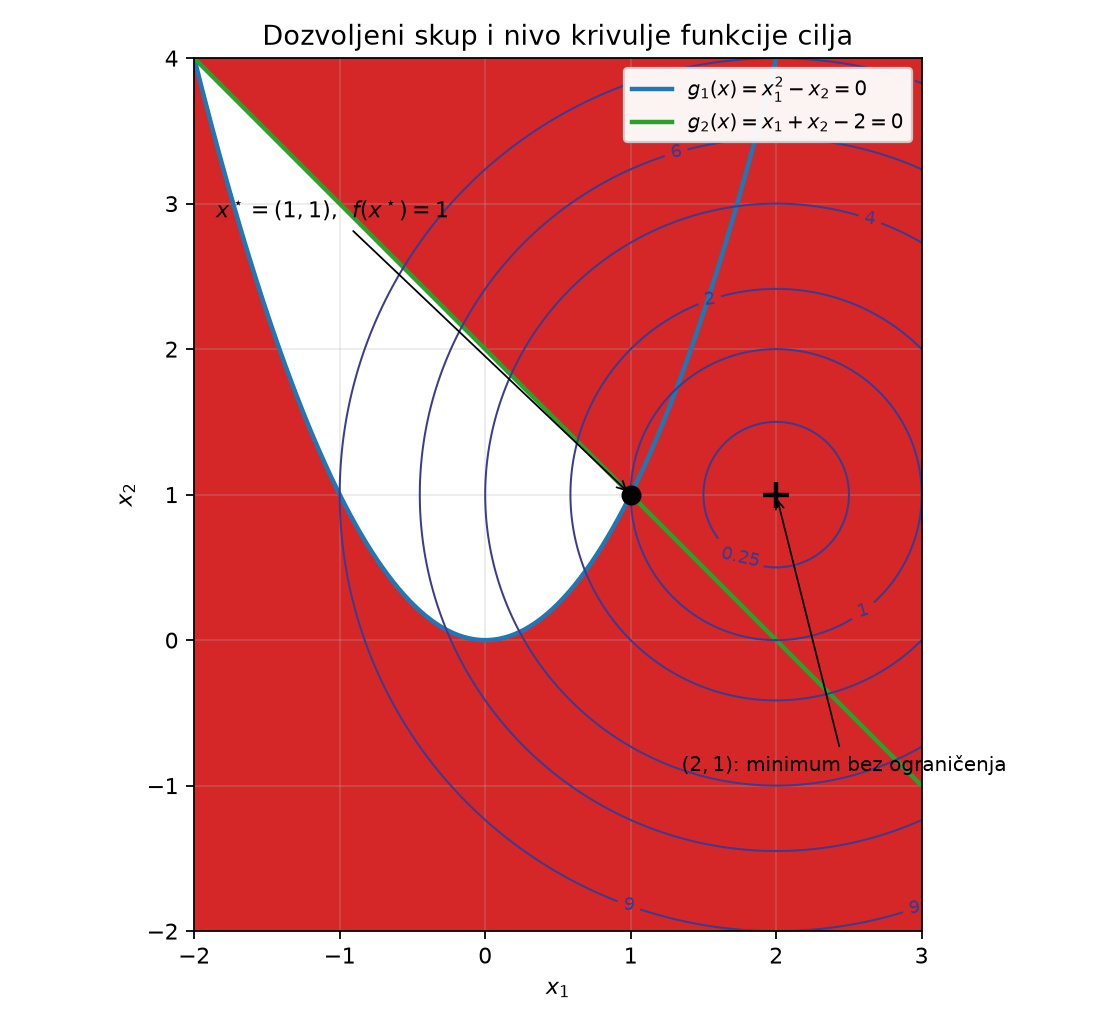
\includegraphics[width=0.86\textwidth]{01-uvodni-primjer.png}
\caption{Dozvoljeni skup (bijela „leća”), nivo krivulje funkcije cilja
(koncentrične kružnice oko $(2,1)$) i optimum $x\opt=(1,1)$.
Nedopušteno područje je crveno.}
\end{figure}

\begin{napomena}[tiskarska pogreška na slajdu 15]
Na slajdu 15 prvo ograničenje je otipkano kao $g_1(x) = x_1^2 - x^2 \le 0$, dok
na slajdovima 10--14 svugdje piše $g_1(x) = x_1^2 - x_2 \le 0$. Ispravno je
$x_1^2 - x_2$ --- to potvrđuje i sam crtež na slajdu (parabola $x_2 = x_1^2$) i
rješenje $x\opt = (1,1)$.
\end{napomena}

% =====================================================================
\section{Gdje i zašto se optimira?}
\str{16--17}

\subsection{Optimiranje rada sustava / procesa („on-line”)}
\begin{itemize}
  \item Planiranje proizvodnje u elektroenergetskoj mreži
  \item Upravljanje motorom automobila
  \item Upravljanje tokovima snage i energijom u hibridnom automobilu
  \item Traženje najkraćeg puta (npr.\ GPS u autu, „preračunavam”)
  \item Gibanje robota prilikom obavljanja zadatka
  \item Plan bušenja rupa na ploči za elektroniku
  \item Web tražilica
  \item Optimalno upravljanje dinamičkim sustavima (bogata inženjerska /
        znanstvena grana za sebe)
  \item \dots
\end{itemize}

\subsection{U fundamentalnim fizikalnim zakonima / problemima}
\begin{itemize}
  \item Traženje \textbf{ravnotežnog položaja} minimizacijom potencijalne
        energije
  \item \textbf{Stabilnost dinamičkih sustava} --- traženje Ljapunovljeve
        funkcije
\end{itemize}

Ove dvije stavke nisu samo ilustracija: prva se detaljno rješava u
poglavlju~\ref{ch:uvjeti}, a druga je tema cijelog poglavlja~\ref{ch:dinamicki}.

\subsection{U prirodi}
\begin{itemize}
  \item Oblik stabla (optimiranje oblika obzirom na vlastitu težinu i vanjska
        opterećenja)
  \item Struktura kosti
  \item Trajektorija šišmiša u lovu na plijen
  \item Oblik jabuke
  \item Prilagodba vrste na uvjete života u zadanoj okolini
  \item \dots
\end{itemize}

\subsection{Optimalno projektiranje}
\begin{itemize}
  \item Optimalna raspodjela vjetroturbina u vjetroparku
  \item Optimiranje topologije, oblika, dimenzija mehanizama i nosivih
        konstrukcija --- \textbf{u ovom kolegiju}
  \item \dots
\end{itemize}

\dots\ i još puno, puno toga.

% =====================================================================
\section{Sadržaj kolegija i ishodi učenja}
\str{18--32}

Kompletan popis tema sa slajdova (gradi se inkrementalno kroz 15 slajdova):

\begin{enumerate}
  \item \textbf{Uvod}: Ciljevi kolegija i ishodi učenja.
  \item \textbf{Optimizacijski problem}: definicije i klasifikacija. Konveksni
        opt.\ problemi.
  \item \textbf{Uvjeti optimalnosti.} Geometrijska interpretacija i primjene.
  \item \textbf{Lagrangeova dualnost}, alternative i analiza osjetljivosti.
  \item \textbf{Linearno programiranje.} Pristupi rješavanju i primjeri.
  \item \textbf{Kvadratno programiranje} s primjenama. Formulacija i značajke.
  \item \textbf{Linearne matrične nejednadžbe i semidefinitno programiranje.}
  \item \textbf{Numerički algoritmi} za rješavanje opt.\ problema (pregled).
  \item \textbf{Optimiranje mehatroničkih sustava} --- od linearnog do
        semidefinitnog programiranja: primjeri iz prakse.
  \item \textbf{Formulacija stabilnosti i disipativnost dinamičkih sustava} kao
        opt.\ problema.
  \item Formulacije kriterija i analiza učinkovitosti dinamičkih sustava.
  \item Formulacije \textbf{optimalnog upravljanja} i pristupi rješavanju.
  \item \textbf{Robusno optimiranje 1}
  \item \textbf{Robusno optimiranje 2}
  \item \textbf{Višeciljna optimizacija} i višeciljno upravljanje
\end{enumerate}

\textbf{Kako se to preslikava na ovu skriptu:} teme 1--2 $\to$
poglavlja~\ref{ch:uvod}--\ref{ch:definicije}; tema 3 $\to$
poglavlje~\ref{ch:uvjeti}; tema 4 $\to$ poglavlje~\ref{ch:dualnost}; teme 5--6
$\to$ poglavlje~\ref{ch:lpqp}; teme 7 i 9 $\to$ poglavlje~\ref{ch:qcpsdp}; teme
10--12 $\to$ poglavlje~\ref{ch:dinamicki}; teme 13--14 $\to$
poglavlje~\ref{ch:robusno}.

% =====================================================================
\section{Motivacijski primjeri iz prakse}
\str{33--43}

\subsection{Planiranje proizvodnje u elektroenergetskoj mreži}
\str{33--34}

\textbf{Problem:} planiranje rada električnih generatora.

Sa slajda, sa svrstavanjem svake stavke u element standardne forme:

\begin{center}
\begin{tabular}{p{7.4cm}p{6.0cm}}
\toprule
\textbf{Sa slajda} & \textbf{Element opt.\ problema} \\
\midrule
tipično noć prije dana proizvodnje & (vremenski okvir odluke) \\
proizvodnja $=$ predviđenoj potrošnji & \textbf{ograničenje jednakosti} $h(x)=0$ \\
minimiziranje troškova proizvodnje & \textbf{funkcija cilja} $f(x)$ \\
ograničenja na tok snage u dalekovodima & \textbf{ograničenja nejednakosti} $g(x)\le 0$ \\
planovi u slučaju kvara & \textbf{robusnost} (poglavlje~\ref{ch:robusno}) \\
\bottomrule
\end{tabular}
\end{center}

Dodatno \str{34}:
\begin{itemize}
  \item Optimiranje (optimalno upravljanje) je \textbf{„skrivena tehnologija”}
        za razvoj naprednih mreža u budućnosti.
  \item Matematička formulacija tržišta i kreiranja tržišnih cijena:
        \textbf{Lagrangeova dualnost}.
\end{itemize}

Zadnja rečenica je najava Vježbi 3, gdje se cijeli „Primjer 1: Tržište i
formiranje cijena” rješava upravo preko dualnosti --- vidi
poglavlje~\ref{ch:dualnost}.

\subsection{Upravljanje tokovima snage i energijom u hibridnom automobilu}
\str{35}

\begin{itemize}
  \item Nije dobro imati napunjenu bateriju: želimo je (polu)praznu da bismo je
        mogli puniti prilikom kočenja (rekuperacija).
  \item \textbf{dobro $\to$ optimalno}
  \item Optimiranje je „skrivena tehnologija” koja daje „inteligenciju”
        procesu: pojmovi \emph{dobro--loše} moraju biti vezani uz neki kriterij
        $\to$ \textbf{formalizacija funkcije cilja}.
\end{itemize}

\subsection{Prediktivno upravljanje dinamičkim sustavima}
\str{36--37}

Slajdovi su ilustracija koncepta MPC-a (engl.\ \emph{Model Predictive
Control}): u svakom koraku se, na temelju modela, riješi optimizacijski problem
na konačnom horizontu predikcije, primijeni se prvi upravljački potez, pa se
postupak ponovi.

\subsection{Optimalno upravljanje --- pozicioniranje glave tvrdog diska}
\str{38}

Slajd prikazuje mehanizam tvrdog diska (ruka s glavom, \emph{pivot},
\emph{voice coil motor} VCM) i regulacijsku petlju: regulator $K$ prima signal
pogreške $e$ i daje upravljanje $u$; $y_r$ je referenca, $y$ izlaz, $d$
poremećaj.

Podaci sa slajda: ${>}15\,000$ o/min, $12\,000$ traka na $1$ cm.

\textbf{Formulacija problema (sa slajda):}
\begin{equation}
\min_K \; \max_{\|d\| \ne 0} \frac{\|e\|}{\|d\|}, \qquad
K \in \{\,\text{stabilizirajući regulatori}\,\}
\end{equation}

\textbf{Kako to čitati.} $\|\cdot\|$ je \textbf{norma} --- mjera „veličine”
signala (formalno u poglavlju~\ref{ch:definicije}). Omjer $\|e\|/\|d\|$ je
„koliko se poremećaj $d$ pojača u pogrešku $e$”. Unutarnji $\max$ uzima
\textbf{najgori mogući} poremećaj, a vanjski $\min$ bira regulator koji taj
najgori slučaj čini što manjim. Ovakav \textbf{min--max} zapis je tipičan za
robusno projektiranje i vratit ćemo mu se u
poglavljima~\ref{ch:dinamicki}~i~\ref{ch:robusno}.

\subsection{Ravnotežni položaj sustava u potencijalnom polju}
\str{39--40}

\textbf{Postavka} \str{39}\textbf{.} Točka mase $m$ obješena je u vertikalnoj
ravnini o dvije elastične opruge zanemarive mase s konstantama $k_1$, $k_2$ i
duljinama $l_1$, $l_2$, dok je razmak objesišta jednak $d$.

Geometrija sa slajda: koordinatni sustav $(x, y)$; lijevo objesište je u
ishodištu $(0,0)$, desno objesište je na osi $x$ na udaljenosti $d$, tj.\ u
$(d, 0)$; masa $m$ visi ispod, u točki $(x, y)$ (s $y < 0$). Lijeva opruga ima
parametre $k_1, l_1$, desna $k_2, l_2$.

\textbf{Zadatak:} izračunati ravnotežni položaj mase.

\textbf{Rješenje} \str{40}\textbf{.} Potencijalna energija mase $m$ u položaju
$(x,y)$ je
\begin{equation}
V(x,y) = mgy
+ \frac{k_1}{2}\left(l_1 - \sqrt{x^2 + y^2}\right)^2
+ \frac{k_2}{2}\left(l_2 - \sqrt{(d-x)^2 + y^2}\right)^2
\end{equation}

\textbf{Rastav izraza član po član} (svaki je član oblika „energija”):

\begin{itemize}
  \item $mgy$ --- \textbf{gravitacijska potencijalna energija} mase u polju sile
        teže ($g$ = ubrzanje sile teže). Budući da masa visi ispod osi $x$, $y$
        je negativan pa je taj član negativan --- spuštanjem mase energija pada.
  \item $\sqrt{x^2 + y^2}$ --- trenutna \textbf{duljina lijeve opruge}, tj.\
        udaljenost od objesišta $(0,0)$ do mase $(x,y)$ (Pitagorin poučak).
  \item $l_1 - \sqrt{x^2+y^2}$ --- \textbf{deformacija} lijeve opruge (razlika
        nedeformirane duljine $l_1$ i trenutne duljine).
  \item $\frac{k_1}{2}(\cdot)^2$ --- \textbf{elastična energija} lijeve opruge;
        standardna formula $E = \tfrac{1}{2}k\,\Delta l^2$.
  \item Analogno za desnu oprugu, samo je njezino objesište u $(d, 0)$, pa je
        udaljenost do mase $\sqrt{(d-x)^2 + y^2}$.
\end{itemize}

\textbf{Ravnotežna točka} $(x\opt, y\opt)$ je ona koja \textbf{minimizira}
potencijalnu energiju:
\begin{equation}
(x\opt, y\opt) = \argmin_{x,\,y} \; V(x,y)
\end{equation}

\begin{napomena}[notacija $\argmin$]
$\min_x V(x)$ je \textbf{najmanja vrijednost} koju $V$ poprima (broj), dok je
$\argmin_x V(x)$ \textbf{argument} u kojem se taj minimum postiže (točka). Za
nas je obično zanimljiv $\argmin$ --- želimo znati \emph{gdje} je optimum, a ne
samo \emph{koliko} iznosi.
\end{napomena}

Ovo je važan konceptualni primjer: \textbf{fizikalni zakon (ravnoteža) izražen
je kao optimizacijski problem bez ograničenja.} Isti primjer se u
poglavlju~\ref{ch:uvjeti} proširuje na slučaj s ograničenjima i rješava preko
uvjeta optimalnosti.

\subsection{Primjeri iz prirode}
\str{41}

Slajd je fotografska ilustracija tvrdnji iz odjeljka o prirodi (oblici koje
priroda „optimira”). Nema dodatnih formula.

\subsection{Raspodjela vjetroturbina u vjetroparku}
\str{42--43}

Slajd 43 prikazuje dva 3D grafa (površina prinosa nad tlocrtom parka, s
ucrtanim pozicijama turbina kao točkama i označenim smjerom sjevera \textbf{N}):

\begin{itemize}
  \item lijevo: \textbf{optimalni položaji sa zanemarenim interakcijama preko
        vrtloga},
  \item desno: \textbf{optimalni položaji s uračunatim interakcijama preko
        vrtloga}.
\end{itemize}

\textbf{Poanta:} ista funkcija cilja (ukupna proizvedena energija), ali bogatiji
model (uzimanje u obzir da turbina u vjetrenoj sjeni druge turbine daje manje)
daje \textbf{bitno drukčiji optimalni raspored}. Model ulazi u optimizaciju
kroz ograničenja i funkciju cilja --- kvaliteta modela izravno određuje
kvalitetu optimuma.

% =====================================================================
\section{Primjer: problem proizvodnje i distribucije robe}
\str{44--45}

Ovo je prvi potpuno formuliran „inženjersko-poslovni” problem u kolegiju i
ujedno prvi primjer \textbf{linearnog programa} (LP), koji ćemo formalno
obraditi u poglavlju~\ref{ch:lpqp}.

\subsection{Opis problema}
\str{44}

\begin{itemize}
  \item Tvrtka ima \textbf{2 tvornice} i \textbf{7 trgovina}.
  \item U jednom proizvodnom vremenskom intervalu tvornica $i$ može proizvesti
        do $a_i$ tona.
  \item Svaka trgovina $j$ redovito ima potražnju od $b_j$ tona.
  \item Troškovi transporta od tvornice $i$ do trgovine $j$ su $c_{ij}$
        kuna/toni.
  \item \textbf{Kako optimalno voditi tvrtku (minimizirati trošak)?}
\end{itemize}

\subsection{Projektne varijable}
\str{45}

\[
x_{ij} \in \R: \text{ koliko tvornica } i \text{ dobavlja robe trgovini } j,
\qquad x_{ij} \ge 0
\]

Budući da imamo $2$ tvornice i $7$ trgovina, ukupno je $2 \times 7 = 14$
varijabli. Uvjet $x_{ij} \ge 0$ je fizikalne prirode: ne može se isporučiti
negativna količina.

\subsection{Potpuna formulacija}
\str{45}

\begin{equation}
\begin{aligned}
\min \quad & \sum_{i=1}^{2} \sum_{j=1}^{7} c_{ij} x_{ij} \\
\uzogr & \sum_{j=1}^{7} x_{ij} \le a_i, \qquad i = 1, 2 \\
       & \sum_{i=1}^{2} x_{ij} \ge b_j, \qquad j = 1, \dots, 7 \\
       & x_{ij} \ge 0
\end{aligned}
\end{equation}

\textbf{Čitanje svakog retka:}

\begin{itemize}
  \item \textbf{Funkcija cilja} $\sum_i \sum_j c_{ij} x_{ij}$: za svaku moguću
        relaciju tvornica $\to$ trgovina pomnožimo prevezenu količinu $x_{ij}$
        [t] s jediničnim troškom $c_{ij}$ [kn/t] i sve zbrojimo. Rezultat je
        \textbf{ukupan trošak transporta} u kunama. (Simbol $\sum$ znači
        „zbroji po svim vrijednostima indeksa”; dvostruka suma znači da
        prolazimo po svim parovima $(i,j)$, dakle po svih 14 relacija.)
  \item \textbf{Kapacitet tvornice} $\sum_{j} x_{ij} \le a_i$: sve što tvornica
        $i$ pošalje (zbroj po svim trgovinama) ne smije prijeći njezin kapacitet
        $a_i$. Dva takva ograničenja (po jedno za svaku tvornicu).
  \item \textbf{Potražnja trgovine} $\sum_{i} x_{ij} \ge b_j$: sve što trgovina
        $j$ primi (zbroj po objema tvornicama) mora biti barem $b_j$. Sedam
        takvih ograničenja.
  \item \textbf{Nenegativnost} $x_{ij} \ge 0$: 14 ograničenja.
\end{itemize}

\begin{napomena}[prevođenje u standardnu formu]
Standardna forma traži $g_j(x)\le 0$, pa nejednakost „$\ge$” pomnožimo s $-1$
(što okreće smjer): $\sum_i x_{ij} \ge b_j \Leftrightarrow
b_j - \sum_i x_{ij} \le 0$, i $x_{ij} \ge 0 \Leftrightarrow -x_{ij} \le 0$.
Kapacitet je već u pravom obliku nakon premještanja:
$\sum_j x_{ij} - a_i \le 0$.
\end{napomena}

Uočite: i funkcija cilja i sva ograničenja su \textbf{linearne} funkcije
varijabli $x_{ij}$. To je definicija linearnog programa
(poglavlje~\ref{ch:lpqp}).

% =====================================================================
\section{Klasični primjeri optimiranja s potpunim rješenjima}
\str{46--52}

Slajdovi 46--52 rješavaju šest školskih ekstremalnih problema. Svi se rješavaju
istim receptom, pa ga vrijedi jednom izreći:

\begin{definicija}[Recept klasične analize --- ekstrem funkcije jedne varijable]
\begin{enumerate}
  \item Uvedi varijablu i izrazi \textbf{funkciju cilja} preko nje.
  \item Ako postoji ograničenje jednakosti, iz njega \textbf{izrazi jednu
        varijablu} i \textbf{uvrsti} u funkciju cilja (eliminacija) --- tako
        problem s ograničenjem postaje problem bez ograničenja.
  \item Deriviraj i izjednači s nulom: $\dfrac{\dd F}{\dd x} = 0$ $\to$
        \textbf{stacionarne točke}.
  \item Provjeri drugom derivacijom: $F'' > 0$ $\to$ \textbf{minimum},
        $F'' < 0$ $\to$ \textbf{maksimum}.
  \item Izračunaj vrijednost cilja u nađenoj točki.
\end{enumerate}
\end{definicija}

Ovaj recept vrijedi za jednostavne, glatke probleme jedne varijable. U
poglavlju~\ref{ch:uvjeti} generalizirat ćemo ga na više varijabli i na probleme
gdje se ograničenja \emph{ne mogu} tako lako eliminirati --- tada nastupaju
Lagrangeovi multiplikatori i KKT uvjeti.

\subsection{Optimalno iskorištavanje materijala --- posuda iz limene ploče}
\str{46--47}

\textbf{Problem.} Iz kvadratne limene ploče stranice $a$ potrebno je izrezati
uglove tako da se iz preostalog dijela načini posuda što većeg volumena.
Izrezuju se četiri kvadratića stranice $x$ u uglovima; preostali „križ” se
savine prema gore.

\textbf{Ciljna funkcija je volumen:}
\[
V = (a - 2x)^2 \cdot x
\]

\emph{Odakle to:} nakon izrezivanja uglova stranice $x$ i savijanja, baza posude
je kvadrat stranice $a - 2x$ (s obje strane oduzimamo po $x$), a visina posude
je $x$.

\textbf{Derivacija:}
\[
\frac{\dd V}{\dd x} = 12x^2 - 8ax + a^2
\]

\emph{Provjera računa} (raspis međukoraka koji na slajdu nije napisan):
\begin{align}
V &= x(a-2x)^2 = x(a^2 - 4ax + 4x^2) = a^2 x - 4a x^2 + 4x^3 \\
\frac{\dd V}{\dd x} &= a^2 - 8ax + 12x^2 \quad \checkmark
\end{align}

\textbf{Izjednačavanje s nulom} daje kvadratnu jednadžbu
$12x^2 - 8ax + a^2 = 0$, čija su rješenja (sa slajda):
\[
x_{1,2} = \frac{a}{3} \pm \frac{a}{6}; \qquad x_1 = a/2, \quad x_2 = a/6
\]

\emph{Provjera preko formule za kvadratnu jednadžbu:}
\begin{align}
x_{1,2} &= \frac{8a \pm \sqrt{(8a)^2 - 4\cdot 12 \cdot a^2}}{2 \cdot 12}
= \frac{8a \pm \sqrt{64a^2 - 48a^2}}{24}
= \frac{8a \pm \sqrt{16a^2}}{24}
= \frac{8a \pm 4a}{24} \\
x_1 &= \frac{12a}{24} = \frac{a}{2}, \qquad
x_2 = \frac{4a}{24} = \frac{a}{6} \quad \checkmark
\end{align}

\textbf{Provjera drugom derivacijom:}
\[
V'' = \frac{\dd^2 V}{\dd x^2} = 24x - 8a
\]
\begin{align}
V''\!\left(\tfrac{a}{2}\right) &= 24 \cdot \tfrac{a}{2} - 8a = 12a - 8a = 4a > 0
\;\to\; \textbf{min.} \\
V''\!\left(\tfrac{a}{6}\right) &= 24 \cdot \tfrac{a}{6} - 8a = 4a - 8a = -4a < 0
\;\to\; \textbf{max.}
\end{align}

\textbf{Vrijednosti:}
\[
V_{\max} = \left(a - \frac{a}{3}\right)^{2} \cdot \frac{a}{6} = \frac{2}{27}a^3;
\qquad V_{\min} = 0
\]

\emph{Provjera:} za $x = a/6$ je $a - 2x = a - a/3 = \tfrac{2a}{3}$, pa je
$V = \left(\tfrac{2a}{3}\right)^2 \cdot \tfrac{a}{6}
= \tfrac{4a^2}{9}\cdot\tfrac{a}{6} = \tfrac{4a^3}{54} = \tfrac{2a^3}{27}$
\checkmark. Za $x = a/2$ je $a - 2x = 0$, pa je $V = 0$ --- geometrijski jasno:
izrezali smo cijelu ploču, baza je nestala.

\subsection{Minimizacija troškova izgradnje --- tlocrt kuće}
\str{48}

\textbf{Problem.} Kuća ima 3 prostorije površine $A$ [m\textsuperscript{2}].
Troškovi izgradnje vanjskih zidova iznose $C$ [EUR/m], a troškovi za
unutrašnje zidove iznose $2/3$ tih troškova. Odrediti mjere tlocrta tako da
troškovi izgradnje zidova budu minimalni.

Geometrija sa slajda: pravokutnik širine $x$ i visine $y$; unutar njega jedan
okomiti zid (duljine $y$) koji odvaja desni dio, te u lijevom dijelu vodoravni
zid duljine $2x/5$ --- tako se dobiju 3 prostorije.

\textbf{Ograničenje jednakosti:}
\[
A = x\,y \; [\text{m}^2] \quad \to \quad y = A/x
\]

\textbf{Ciljna funkcija $\to$ minimalni troškovi:}
\[
F(x) = C\left(2x + 2\frac{A}{x}\right)
     + \frac{2}{3}C\left(\frac{2}{5}x + \frac{A}{x}\right)
\]

\emph{Rastav:} prvi član su vanjski zidovi --- opseg pravokutnika je
$2x + 2y = 2x + 2A/x$, uz cijenu $C$. Drugi član su unutarnji zidovi ---
vodoravni duljine $\tfrac{2}{5}x$ i okomiti duljine $y = A/x$, uz cijenu
$\tfrac{2}{3}C$.

\textbf{Sređivanje (sa slajda):}
\[
F(x) = \frac{2}{3}C\left(\frac{17}{5}x + 4\frac{A}{x}\right)
\]

\emph{Raspis međukoraka koji na slajdu nije prikazan:}
\begin{align}
F(x) &= 2Cx + \frac{2CA}{x} + \frac{2}{3}C \cdot \frac{2}{5}x
        + \frac{2}{3}C\frac{A}{x} \\
     &= C\underbrace{\left(2 + \frac{4}{15}\right)}_{=\frac{30+4}{15}=\frac{34}{15}}x
      + C\underbrace{\left(2 + \frac{2}{3}\right)}_{=\frac{6+2}{3}=\frac{8}{3}}\frac{A}{x}
      = \frac{34}{15}Cx + \frac{8}{3}C\frac{A}{x}
\end{align}
a s druge strane
\[
\frac{2}{3}C\left(\frac{17}{5}x + \frac{4A}{x}\right)
= \frac{2 \cdot 17}{3 \cdot 5}Cx + \frac{2\cdot 4}{3}C\frac{A}{x}
= \frac{34}{15}Cx + \frac{8}{3}C\frac{A}{x} \quad \checkmark
\]

\textbf{Konstante prebacimo na lijevu stranu} (jer konstantni pozitivni faktor
ne mijenja položaj minimuma --- ovo je važan i često korišten trik):
\[
F_0 = \frac{3F(x)}{2C} = \left(\frac{17}{5}x + 4\frac{A}{x}\right)
\]

\textbf{Derivacija i izjednačavanje s nulom:}
\[
\frac{\dd F_0}{\dd x} = \frac{17}{5} - \frac{4A}{x^2} = 0
\quad \to \quad x^2 = \frac{20}{17}A = \frac{20}{17}xy
\]

\emph{Međukorak:} iz $\tfrac{17}{5} = \tfrac{4A}{x^2}$ slijedi
$x^2 = \tfrac{4A \cdot 5}{17} = \tfrac{20A}{17}$; zatim se uvrsti $A = xy$.

\textbf{Odakle treba biti:}
\[
\frac{x}{y} = \frac{20}{17}
\]

\emph{Međukorak:} iz $x^2 = \tfrac{20}{17}xy$ podijelimo obje strane s $x$
(dopušteno jer $x > 0$) i dobijemo $x = \tfrac{20}{17}y$, tj.\ $x/y = 20/17$.

\subsection{Maksimizacija volumena lijevka I}
\str{49}

\textbf{Problem.} Neka se iz okrugle ploče izreže isječak tako da se iz ostatka
načini lijevak (stožac) što većeg volumena.

Geometrija: iz kruga polumjera $r$ izreže se kružni isječak, a preostali dio
(središnjeg kuta $\varphi$) se smota u plašt stošca. Nastali stožac ima polumjer
baze $R$, izvodnicu $r$ (jer je to polumjer polazne ploče) i visinu $h$.

\textbf{Polumjer baze (1):} duljina luka preostalog dijela postaje opseg baze:
\begin{equation}
2R\pi = r\varphi \quad \to \quad R = \frac{r\varphi}{2\pi}
\end{equation}

\textbf{Visina stošca (2):} iz pravokutnog trokuta (izvodnica, polumjer baze,
visina):
\begin{equation}
h = \sqrt{r^2 - R^2}
\end{equation}

\textbf{Ciljna funkcija (3):} volumen stošca
\begin{equation}
V = \frac{\pi R^2 h}{3}
\end{equation}

\textbf{Uvrštenjem (1) i (2) u (3):}
\[
V = \frac{r^3}{12\pi}\varphi^2 \sqrt{1 - \frac{\varphi^2}{4\pi^2}}
\]

\emph{Raspis međukoraka:}
\begin{align}
R^2 &= \frac{r^2\varphi^2}{4\pi^2}, \qquad
h = \sqrt{r^2 - \frac{r^2\varphi^2}{4\pi^2}}
  = r\sqrt{1 - \frac{\varphi^2}{4\pi^2}} \\
V &= \frac{\pi}{3}\cdot\frac{r^2\varphi^2}{4\pi^2}\cdot
     r\sqrt{1 - \frac{\varphi^2}{4\pi^2}}
   = \frac{r^3\varphi^2}{12\pi}\sqrt{1 - \frac{\varphi^2}{4\pi^2}}
   \quad \checkmark
\end{align}

\textbf{Prebacivanjem konstanti na lijevu stranu i kvadriranjem, uređena ciljna
funkcija je:}
\[
F(\varphi) = \left(\frac{12\pi V}{r^3}\right)^{2}
= \varphi^4\left(1 - \frac{\varphi^2}{4\pi^2}\right)
\]

\begin{napomena}[zašto smijemo kvadrirati]
Funkcija $t \mapsto t^2$ je \textbf{strogo rastuća} za $t \ge 0$, a $V \ge 0$.
Strogo rastuća transformacija ne mijenja \emph{položaj} maksimuma, samo njegovu
vrijednost. Isto vrijedi za množenje pozitivnom konstantom. Ovaj postupak
(uklanjanje korijena kvadriranjem) koristit ćemo često --- vidi i Vježbe 2, gdje
se isto radi s normama.
\end{napomena}

\textbf{Derivacija:}
\[
\frac{\dd F}{\dd \varphi} = 4\varphi^3 - \frac{3}{2\pi^2}\varphi^5 = 0
\]

\emph{Provjera:} $F(\varphi) = \varphi^4 - \dfrac{\varphi^6}{4\pi^2}$, pa je
$F' = 4\varphi^3 - \dfrac{6\varphi^5}{4\pi^2}
    = 4\varphi^3 - \dfrac{3\varphi^5}{2\pi^2}$ \checkmark

\textbf{Iz toga slijedi:}
\[
\varphi^2 = \frac{8}{3}\pi^2 \quad \to \quad
\varphi = \sqrt{\frac{2}{3}}\cdot 2\pi \,\text{rad} = 293{,}939^\circ
\]

\emph{Međukoraci:} podijelimo jednadžbu s $\varphi^3$ (za $\varphi \ne 0$):
$4 = \tfrac{3}{2\pi^2}\varphi^2$, dakle $\varphi^2 = \tfrac{8\pi^2}{3}$. Zatim
$\varphi = \sqrt{\tfrac{8\pi^2}{3}} = 2\pi\sqrt{\tfrac{2}{3}}$. Brojčano:
$\sqrt{2/3} = 0{,}8165$, pa $\varphi = 0{,}8165 \cdot 6{,}2832 = 5{,}1302$ rad;
u stupnjevima $5{,}1302 \cdot \tfrac{180}{\pi} = 293{,}94^\circ$ \checkmark

\subsection{Maksimizacija volumena lijevka II}
\str{50}

\textbf{Problem.} Kakav oblik treba imati lijevak (stožac) da kod \textbf{zadane
površine plašta} ima što veći volumen?

\textbf{Površina plašta:}
\[
A = 2\pi r \cdot R / 2 = \pi R r \quad \to \quad r = \frac{A}{\pi R}
\]

(Ovdje je $r$ izvodnica stošca, $R$ polumjer baze.)

\textbf{Volumen:}
\[
V = \frac{\pi R^2}{3}\sqrt{r^2 - R^2}
  = \frac{\pi R^2}{3}\sqrt{\frac{A^2}{\pi^2R^2} - R^2}, \qquad
V = \frac{R}{3}\sqrt{A^2 - \pi^2R^4}
\]

\emph{Raspis zadnjeg koraka:} izlučimo $\tfrac{1}{\pi^2R^2}$ iz korijena:
\begin{align}
\sqrt{\frac{A^2}{\pi^2R^2} - R^2} &= \frac{1}{\pi R}\sqrt{A^2 - \pi^2 R^4} \\
V &= \frac{\pi R^2}{3}\cdot\frac{1}{\pi R}\sqrt{A^2 - \pi^2R^4}
   = \frac{R}{3}\sqrt{A^2 - \pi^2R^4} \quad \checkmark
\end{align}

\textbf{Volumen $V$ bit će maksimalan kad i $(3V)^2$}, pa je (isti trik kao
prije):
\[
F(R) = (3V)^2 = A^2R^2 - \pi^2R^6
\]

\textbf{Derivacija:}
\[
\frac{\dd F}{\dd R} = 2A^2R - 6\pi^2R^5 = 0 \quad \to \quad
A = \sqrt{3\pi^2R^4} = \pi\sqrt{3}\,R^2
\]

\emph{Međukorak:} podijelimo s $2R$ ($R \ne 0$): $A^2 = 3\pi^2R^4$, pa
korjenovanjem $A = \pi R^2\sqrt{3}$.

\textbf{Iz $R^2 = \dfrac{A}{\pi\sqrt{3}}$ i
$h^2 = r^2 - R^2 = \dfrac{A^2}{\pi^2R^2} - R^2$, slijedi:}
\[
\frac{h^2}{R^2} = 2 \quad \to \quad \frac{h}{R} = \sqrt{2}
\]

\emph{Raspis:}
\[
\frac{h^2}{R^2} = \frac{1}{R^2}\left(\frac{A^2}{\pi^2R^2} - R^2\right)
= \frac{A^2}{\pi^2R^4} - 1
\overset{A^2 = 3\pi^2R^4}{=} \frac{3\pi^2R^4}{\pi^2R^4} - 1 = 3 - 1 = 2
\quad \checkmark
\]

\textbf{Zaključak:} optimalan lijevak ima omjer visine i polumjera baze
$h/R = \sqrt{2}$.

\subsection{Dimenzioniranje otvora vrata}
\str{51}

\textbf{Problem.} Kako visoka moraju biti vrata tornja ($h$) da se ljestve
duljine $L$ mogu uvući u toranj?

Geometrija sa slajda: zid tornja je okomit; ljestve $\overline{AB} = L$
naslonjene su tako da im donji kraj $B$ klizi po podu na udaljenosti $x$ od
zida, a gornji kraj $A$ je uz vanjski zid; $a$ je vodoravni odmak zida, $y$ je
visina na kojoj ljestve prelaze preko brida vrata, a $h$ je tražena visina
vrata.

\textbf{Rješenje:} traži se \textbf{maksimalna visina $y$ za vrijeme uvlačenja}
ljestvi u toranj.

\textbf{Iz sličnosti trokuta (1):}
\begin{equation}
\frac{y}{x-a} = \frac{\sqrt{L^2 - x^2}}{x}
\quad \to \quad
y = \frac{x-a}{x}\sqrt{L^2 - x^2}
\end{equation}

(Ovdje je $\sqrt{L^2 - x^2}$ visina gornjeg kraja ljestvi $A$ nad podom ---
Pitagorin poučak na trokutu s hipotenuzom $L$ i vodoravnom katetom $x$.)

\textbf{Derivacija i stacionarna točka (2):}
\begin{equation}
\frac{\dd y}{\dd x} = \frac{aL^2 - x^3}{x^2\sqrt{L^2 - x^2}} = 0
\quad \to \quad x_{\mathrm m} = \sqrt[3]{aL^2}
\end{equation}

\emph{Međukorak:} razlomak je nula kad je brojnik nula: $aL^2 - x^3 = 0
\Rightarrow x^3 = aL^2 \Rightarrow x = \sqrt[3]{aL^2}$.

\textbf{Uvrštenjem (2) u (1):}
\[
h \ge y_{\mathrm m} = \left[1 - \left(\frac{a}{L}\right)^{2/3}\right]^{3/2}\cdot L
\]

\emph{Raspis uvrštavanja (na slajdu nije prikazan):} uz
$x_{\mathrm m} = a^{1/3}L^{2/3}$,
\begin{align}
\frac{a}{x_{\mathrm m}} &= \frac{a}{a^{1/3}L^{2/3}} = \frac{a^{2/3}}{L^{2/3}}
= \left(\frac{a}{L}\right)^{2/3} \\
\sqrt{L^2 - x_{\mathrm m}^2} &= \sqrt{L^2 - a^{2/3}L^{4/3}}
= L\sqrt{1 - \left(\frac{a}{L}\right)^{2/3}} \\
y_{\mathrm m} &= \left(1 - \frac{a}{x_{\mathrm m}}\right)
                 \sqrt{L^2 - x_{\mathrm m}^2}
= \left[1 - \left(\tfrac{a}{L}\right)^{2/3}\right]
  \cdot L\left[1 - \left(\tfrac{a}{L}\right)^{2/3}\right]^{1/2}
= L\left[1 - \left(\tfrac{a}{L}\right)^{2/3}\right]^{3/2} \; \checkmark
\end{align}

\textbf{Brojčani primjer sa slajda:}
\[
a = 2{,}7\,\text{m}; \quad L = 12{,}5\,\text{m}
\;\to\; y_{\mathrm m} = 6{,}4\,\text{m}; \quad x_{\mathrm m} = 7{,}5\,\text{m}
\]

\emph{Provjera računa:}
\begin{align}
\frac{a}{L} &= \frac{2{,}7}{12{,}5} = 0{,}216 = 0{,}6^3
\;\Rightarrow\; \left(\frac{a}{L}\right)^{2/3} = 0{,}6^2 = 0{,}36 \\
y_{\mathrm m} &= 12{,}5\,(1 - 0{,}36)^{3/2} = 12{,}5 \cdot 0{,}64^{3/2}
= 12{,}5 \cdot 0{,}8^3 = 12{,}5 \cdot 0{,}512 = 6{,}4\,\text{m} \quad \checkmark \\
x_{\mathrm m} &= \sqrt[3]{2{,}7 \cdot 12{,}5^2} = \sqrt[3]{2{,}7 \cdot 156{,}25}
= \sqrt[3]{421{,}875} = 7{,}5\,\text{m} \quad \checkmark
\end{align}

Slajd uz to prikazuje graf $y(x)$ za te brojke: krivulja kreće od nule pri
$x = a = 2{,}7$, raste do vrha $y \approx 6{,}4$ pri $x = 7{,}5$, i pada natrag
na nulu pri $x = L = 12{,}5$ (tada su ljestve okomite uz zid).

\subsection{Optimalna ograda}
\str{52}

\textbf{Problem.} Površinu od 1 ha treba ograditi na način prema skici
(pravokutnik $x \times y$ s jednim unutarnjim pregradnim zidom duljine $y$).
Troškovi postavljanja ograde proporcionalni su duljini ograde. Odrediti
dimenzije $x$ i $y$ tako da troškovi budu minimalni.

\textbf{Ciljna funkcija je duljina ograde:}
\begin{equation}
L = 2x + 3y
\end{equation}

\emph{Odakle:} vanjski opseg je $2x + 2y$, a unutarnja pregrada je još jedan
komad duljine $y$; ukupno $2x + 3y$.

\textbf{Ograničenje je površina:}
\begin{equation}
A = x\,y = 10\,000\,\text{m}^2 \quad \to \quad h = xy - 10\,000 = 0
\end{equation}

(1 ha $=$ 10\,000 m\textsuperscript{2}. Zapis $h = xy - 10\,000 = 0$ je upravo
standardna forma ograničenja jednakosti iz
odjeljka~\ref{sec:standardna-forma}.)

\textbf{Uvrštenjem (2) u (1)}, tj.\ $y = 10\,000/x$, \textbf{ciljna funkcija
postaje:}
\[
L = 2x + \frac{3 \cdot 10\,000}{x}
\quad \to \quad
\frac{\dd L}{\dd x} = 2 - \frac{30\,000}{x^2} = 0
\]

\textbf{pa je:}
\[
x_{\text{opt}} = 100\sqrt{\frac{3}{2}}, \qquad
y_{\text{opt}} = 100\sqrt{\frac{2}{3}}, \qquad
\left(\frac{x}{y}\right)_{\text{opt}} = \frac{3}{2}
\]

\emph{Raspis:}
\begin{align}
2 &= \frac{30\,000}{x^2} \;\Rightarrow\; x^2 = 15\,000
\;\Rightarrow\; x = \sqrt{15\,000} = \sqrt{10\,000 \cdot 1{,}5}
= 100\sqrt{\tfrac{3}{2}} \approx 122{,}47\,\text{m} \\
y &= \frac{10\,000}{x} = \frac{10\,000}{100\sqrt{3/2}} = \frac{100}{\sqrt{3/2}}
= 100\sqrt{\tfrac{2}{3}} \approx 81{,}65\,\text{m} \\
\frac{x}{y} &= \frac{100\sqrt{3/2}}{100\sqrt{2/3}} = \sqrt{\frac{3/2}{2/3}}
= \sqrt{\frac{9}{4}} = \frac{3}{2} \quad \checkmark
\end{align}

\textbf{Interpretacija:} omjer stranica nije $1{:}1$ (kao kod običnog
pravokutnika bez pregrade) nego $3{:}2$ --- jer pregradni zid „poskupljuje”
smjer $y$, pa se isplati taj smjer skratiti.

% =====================================================================
\section{Vrste optimizacije konstrukcija}
\str{53--56}

\subsection{Dimenzionalna optimizacija (\emph{size optimization})}
\str{53}

Optimiranje \textbf{dimenzija} objekata \textbf{poznate strukture i oblika}.

Primjeri:
\begin{itemize}
  \item dimenzije elemenata nosivih konstrukcija (presjeci štapova, debljine
        limova, \dots)
  \item dimenzije članova mehanizama
\end{itemize}

\subsection{Optimiranje oblika (\emph{shape optimization})}
\str{54}

Osnovni \textbf{oblik} objekta mijenja se postupkom optimizacije ovisno o
zadanim parametrima problema (alat je često \textbf{FEM} analiza --- metoda
konačnih elemenata).

\subsection{Topološka optimizacija (\emph{topology optimization})}
\str{55--56}

Traži se optimalna \textbf{topologija (struktura)} konstrukcije u zadanoj
domeni.

\begin{napomena}
Na slajdovima 55 i 56 topološka optimizacija je numerirana kao „2.” (očit
tipfeler u prezentaciji --- dvije uzastopne stavke nose broj 2). Sadržajno je
to \textbf{treća} vrsta.
\end{napomena}

\textbf{Razlika u tri riječi:} \emph{dimenzionalna} mijenja \textbf{brojeve}
(koliko je štap debeo), \emph{oblikovna} mijenja \textbf{konture} (kako je rub
zaobljen), \emph{topološka} mijenja \textbf{raspored materijala} (gdje uopće ima
materijala, a gdje su rupe). Topološka je najslobodnija i najteža.

% =====================================================================
\section{Postavka problema}
\str{57--58}

\begin{teorem}[Ključna poruka slajda 57]
Pravilna definicija, formulacija i točna matematička postavka optimizacijskog
problema je često \textbf{najveći korak} prilikom rješavanja problema.

Iz formulacije problema treba raspoznati o \textbf{kojoj se vrsti optimizacije
radi}.
\end{teorem}

\subsection{Jednostavan primjer koji to ilustrira}
\str{57--58}

\textbf{Problem.} Površinu uz postojeću prirodnu ogradu (zid, stijena i sl.)
treba ograditi s raspoloživom duljinom žičane ograde $L$ tako da ograđena
površina bude \textbf{maksimalna}.

Na slajdu su prikazana \textbf{tri oblika}:
\begin{itemize}
  \item \textbf{a)} pravokutnik naslonjen na zid (jedna stranica $x$ uz zid,
        dvije stranice $y$),
  \item \textbf{b)} polukrug polumjera $r$ naslonjen na zid,
  \item \textbf{c)} pola pravilnog mnogokuta ($n$-terokut, konkretno $n = 8$)
        naslonjenog na zid.
\end{itemize}

\textbf{Poanta (sa slajda):}

\begin{quote}
Iz gornje formulacije nije jasno da li se oblik ograde može odabrati po volji
ili se postavljaju i neki drugi zahtjevi. Svaki od pokazanih oblika daje za istu
duljinu ograde svoje rješenje, pri čemu se oblikom b) ograđuje \textbf{najveća}
površina, a oblikom a) \textbf{najmanja}. Međutim, ako se radi o ogradi pašnjaka
koju treba seliti duž zida, tada je oblik a) u „tehnološkoj” prednosti, jer se
iskoristi sva raspoloživa površina.
\end{quote}

\textbf{Zaključak:} ista rečenica („ogradi maksimalnu površinu”) daje
\textbf{tri različita optimizacijska problema}, ovisno o tome što smo prešutno
pretpostavili. Zato je formulacija najvažniji korak.

\subsection{Brojčana usporedba triju oblika, $L = 500$ m}
\str{58}

\subsubsection*{Oblik b) --- polukrug}
\[
L = r\pi \;\to\; A = \frac{\pi r^2}{2} = \frac{L^2}{2\pi} = \frac{500^2}{2\pi}
= 39\,788{,}7\,\text{m}^2
\]

\emph{Raspis:} iz $L = r\pi$ slijedi $r = L/\pi$, pa je
$A = \tfrac{\pi}{2}\cdot\tfrac{L^2}{\pi^2} = \tfrac{L^2}{2\pi}
= \tfrac{250\,000}{6{,}2832} = 39\,788{,}7$ m\textsuperscript{2} \checkmark

\subsubsection*{Oblik c) --- polovica pravilnog $n$-terokuta, $n = 8$ (osmerokut)}
\[
L = \frac{n}{2}a \;\to\; \varphi = \frac{2\pi}{n}; \qquad
a = 2r\sin\frac{\varphi}{2} = 2r\sin\frac{\pi}{n}
\]

($a$ je duljina jedne stranice, $\varphi$ središnji kut nad jednom stranicom,
$r$ polumjer opisane kružnice. Uz zid je polovica mnogokuta, pa ograda ima $n/2$
stranica.)

\[
r = \frac{L}{n \cdot \sin\frac{\pi}{n}}
\]

\emph{Raspis:} iz $L = \tfrac{n}{2}a = \tfrac{n}{2}\cdot 2r\sin\tfrac{\pi}{n}
= n\,r\sin\tfrac{\pi}{n}$ slijedi $r = \tfrac{L}{n\sin(\pi/n)}$ \checkmark

\[
A = \frac{1}{2}a\,r\cos\frac{\varphi}{2}\cdot\frac{n}{2}
= \frac{n}{4}\cdot 2\frac{L}{n}\cdot\frac{L}{n\cdot\sin\frac{\pi}{n}}
  \cos\frac{\pi}{n}
= \frac{L^2}{2\,n \cdot \tan\frac{\pi}{n}}
\]

\[
A = \frac{500^2}{2 \cdot 8 \cdot \tan\frac{\pi}{8}} = 37\,722{,}1\,\text{m}^2
\qquad \left(\text{za } n \to \infty, \;
\lim_{n\to\infty}\left(n\cdot\tan\frac{\pi}{n}\right) = \pi\right)
\]

\emph{Provjera brojki:} $\tan(\pi/8) = \tan 22{,}5^\circ = 0{,}41421$, pa je
$2 \cdot 8 \cdot 0{,}41421 = 6{,}6274$ i
$A = 250\,000/6{,}6274 = 37\,722$ m\textsuperscript{2} \checkmark

\emph{Značenje granice:} kad $n \to \infty$, $n\tan(\pi/n) \to \pi$, pa formula
za mnogokut prelazi u $A \to L^2/(2\pi)$ --- točno rezultat polukruga b).
Mnogokut s mnogo stranica je praktički polukrug, što potvrđuje da je b)
najbolji oblik.

\subsubsection*{Oblik a) --- pravokutnik}
\[
L = x + 2y \;\to\; x = L - 2y \quad (\text{ograničenje jednakosti})
\]
\[
A = xy = (L - 2y)\,y; \qquad
\frac{\dd A}{\dd y} = L - 4y = 0 \;\to\;
y = \frac{L}{4} = 125\,\text{m}; \quad x = \frac{L}{2} = 250\,\text{m}
\]

\emph{Raspis derivacije:} $A = Ly - 2y^2$, pa je
$\tfrac{\dd A}{\dd y} = L - 4y$ \checkmark

\[
A = x\,y = 250 \cdot 125 = 31\,250\,\text{m}^2 \qquad (x : y = 2 : 1)
\]

\textbf{Rangiranje:} b) $39\,788{,}7$ $>$ c) $37\,722{,}1$ $>$ a) $31\,250$
m\textsuperscript{2}. Razlika između najboljeg i najlošijeg oblika je oko
\textbf{27\,\%} --- a sve uz istu duljinu ograde. Odabir \emph{strukture}
(oblika) donosi veći dobitak nego optimiranje \emph{dimenzija} unutar zadane
strukture. To je uvod u sljedeći odjeljak.

% =====================================================================
\section{Projektiranje kao proces}
\str{59--77}

\subsection{Slijed projektiranja}
\str{59}

Projektiranje tehničkog sustava ostvaruje se u \textbf{dva koraka}:

\begin{enumerate}
  \item \textbf{izbor strukture} sustava, odnosno \textbf{strukturalne sinteze};
  \item \textbf{izbor brojčanih vrijednosti parametara} odabrane strukture
        (sinteza parametara ili \textbf{dimenzionalna sinteza}).
\end{enumerate}

\begin{quote}
\textbf{Strukturalna sinteza} jest (glavni) zadatak \textbf{stvaralačkog
djelovanja inženjera} koji je općenito teško ili nemoguće automatizirati
(algoritmizirati).
\end{quote}

To se izravno poklapa s primjerom ograde: odabir između oblika a), b), c) je
strukturalna sinteza (kreativni čin), a računanje $x = 250$, $y = 125$ je
dimenzionalna sinteza (algoritamski dio) --- i baš je taj drugi dio ono što ovaj
kolegij formalizira.

\subsection{Strukturalna sinteza}
\str{60}

Struktura projektiranog tehničkog sustava ili objekta (\textbf{topologija
konstrukcije}) određena je poznatim \textbf{skupom elemenata strukture} i
\textbf{vezama među njima}.

\textbf{Poteškoće koje se pojavljuju u formalizaciji problema strukturalne
sinteze:}
\begin{itemize}
  \item nemjerljive karakteristike elemenata strukture;
  \item formalno nedefinirane veze između pojedinih elemenata i zahtjeva;
  \item kvalitativni kriteriji;
  \item neformalan opis funkcioniranja projektiranog objekta;
  \item zahtjevi koji se odnose na funkcioniranje objekta.
\end{itemize}

\textbf{Temelj sinteze tehničkih sustava jest:} skup znanja i iskustva
projektanata, intuicija, kreativnost, literatura, izvedeni projekti, sheme
mogućih rješenja, metode projektiranja, računalna i programska podrška.

Opis elemenata strukture, opis veza među njima kao i formiranje matematičkog
modela strukture definira se pomoću prikladnog (konačnog) skupa veličina: to su
\textbf{projektni parametri}.

\subsection{Cilj projektiranja?}
\str{61--67}

\begin{enumerate}
  \item Gradnja sustava s besprijekornim funkcioniranjem se \textbf{danas
        podrazumijeva}.
  \item U uvjetima konkurencije od presudne je važnosti projektirati
        \textbf{najbolji ili što bolji} sustav (objekt ili proizvod).
  \item Kriteriji po kojima je neki sustav najbolji su različiti, primjerice:
        \textbf{cijena, težina, efikasnost, oblik, praktičnost, kompleksnost,
        originalnost, pouzdanost, trajnost} i sl.
  \item \textbf{Izbor dominantnog kriterija} predstavlja \textbf{stratešku
        odluku} na početku samog procesa projektiranja. Kvaliteta rješenja
        ocjenjuje se \textbf{kvantitativnom} usporedbom odabranih kriterija,
        koji stoga moraju biti \textbf{funkcijom projektnih parametara}.
  \item Izbor projektnih parametara najčešće \textbf{nije slobodan}, već njihove
        veličine moraju zadovoljiti neke unaprijed zadane uvjete ili
        \textbf{ograničenja}. Također trebaju biti ispunjeni uvjeti
        \textbf{međusobne ovisnosti} parametara koji slijede iz strukture
        projektiranog sustava.
  \item Projektiranje je stoga \textbf{iterativni proces} određivanja strukture
        i projektnih parametara projektiranog sustava, konstrukcije ili
        proizvoda.
  \item Konačnim projektnim rješenjem trebaju se ispuniti \textbf{svi} kriteriji
        i tehnički zahtjevi projekta.
\end{enumerate}

Točka 4 je zapravo definicija \textbf{funkcije cilja} rečena inženjerskim
jezikom („kriterij mora biti funkcija projektnih parametara”), a točka 5
definicija \textbf{ograničenja}. Time se zatvara krug s
odjeljkom~\ref{sec:standardna-forma}.

\subsection{Proces projektiranja}
\str{68}

Prema primijenjenim metodama i projektnim zahtjevima proces projektiranja može
biti:

\textbf{a) Proces konvencionalnog projektiranja.} Osnovni cilj: besprijekorno
funkcioniranje sustava ili proizvoda u okviru uvjeta postavljenih projektnim
zadatkom (\emph{funkcionalno projektiranje}). Ovaj proces baziran je na
\textbf{iskustvu i intuiciji}.

\textbf{b) Proces optimalnog projektiranja.} Pored besprijekornog
funkcioniranja sustava ili proizvoda, \textbf{jedan ili više projektnih
kriterija treba biti ispunjen na optimalan način}. Postupak optimalnog
projektiranja zahtijeva \textbf{strogu matematičku formulaciju problema} ---
postavku matematičkog modela ili optimizacijskog problema.

\subsection{Elementi optimizacijskog modela: projektni parametri i varijable}
\str{69--70}

\begin{definicija}[Projektni parametri]
\textbf{Projektni parametri} su veličine pomoću kojih se \textbf{jednoznačno
definiraju dimenzije i svojstva} konstrukcije ili projektiranog sistema.
\end{definicija}

Projektni parametri dijele se na \textbf{konstantne projektne parametre} i
\textbf{projektne varijable}.

\textbf{Konstantni projektni parametri} se u postupku optimizacije \textbf{ne
mijenjaju}, a mogu se podijeliti na dvije vrste:

\begin{itemize}
  \item \textbf{taktički projektni parametri ($z$)} --- zadani su
        \textbf{projektnim zadatkom} i ne mogu se mijenjati u cijelom procesu
        projektiranja. Oni su konstante strukturalne i dimenzionalne sinteze
        konstrukcije, tj.\ predstavljaju \textbf{taktičke performanse}
        projektiranog sustava.
  \item \textbf{tehnički projektni parametri ($y$)} --- projektne su konstante
        \textbf{po zamisli projektanta}, i to prvenstveno iz
        \textbf{konstrukcijskih ili tehnoloških} razloga.
\end{itemize}

\textbf{Hijerarhija sa slajda 70:}

\begin{center}
\begin{tabular}{c}
\toprule
\textbf{PROJEKTNI PARAMETRI} \\
\midrule
\begin{tabular}{p{5.0cm}|p{7.0cm}}
\centering \textbf{PROJEKTNE VARIJABLE} & \centering\textbf{PROJEKTNE KONSTANTE} \tabularnewline
\centering $x$ & \centering $y,\; z$ \tabularnewline
 & \begin{tabular}{p{3.0cm}p{3.0cm}}
   \textbf{TEHNIČKI} $y$ & \textbf{TAKTIČKI} $z$ \\
   (odabrani od projektanta) & (zadani projektnim zadatkom)
   \end{tabular}
\end{tabular} \\
\bottomrule
\end{tabular}
\end{center}

\textbf{Dodatne tvrdnje sa slajda 70:}
\begin{itemize}
  \item Tehnički parametri su konstante \textbf{samo kod dimenzionalne sinteze
        već poznate strukture (topologije)} objekta.
  \item Projektant može mijenjati broj tehničkih parametara njihovim
        \textbf{prebacivanjem u projektne varijable i obrnuto}.
  \item Projektni parametri koji se \textbf{mijenjaju} u postupku sinteze
        nazivaju se \textbf{projektnim varijablama ($x$)}.
  \item \textbf{Suma broja projektnih varijabli i tehničkih parametara} u
        postupku optimizacije iste strukture sistema je \textbf{konstantna}.
  \item Ispravan izbor projektnih parametara i odgovarajuća matematička
        formulacija problema glavne su poteškoće i preduvjeti uspješnog postupka
        optimalnog projektiranja.
\end{itemize}

\begin{napomena}[veza sa standardnom formom]
Vektor $x$ iz standardne forme $=$ projektne varijable. Parametri $y$ i $z$ ne
pojavljuju se kao nepoznanice, nego kao \textbf{brojevi} u izrazima za $f$, $h$
i $g$. U primjeru ograde: $x$ i $y$ (dimenzije) su projektne varijable, a
$10\,000$ m\textsuperscript{2} je taktički parametar (zadan zadatkom).
\end{napomena}

\subsection{Optimizacijski model --- pravila izbora parametara}
\str{71--77}

Kod izbora projektnih parametara važno je sljedeće:

\begin{enumerate}
  \item Projektant treba dobro \textbf{proučiti problem} i matematički ga
        opisati pomoću projektnih varijabli;
  \item Projektni parametri trebaju biti \textbf{nezavisni};
  \item Problem treba opisati sa \textbf{što manje} projektnih parametara;
  \item Matematičku formulaciju problema treba u \textbf{početnoj fazi} provesti
        sa \textbf{što manjim brojem tehničkih parametara}; to je važno radi
        fleksibilnosti algoritma i otklanjanja eventualnih pogrešnih procjena o
        utjecaju nekih tehničkih parametara na rezultat. U \textbf{kasnijoj
        fazi} mogu se neke od varijabli odabrati kao konstante, i to:
        \begin{itemize}
          \item iz \textbf{konstrukcijskih ili tehnoloških} razloga;
          \item jer je utvrđeno da \textbf{ne utječu bitno} na konačni rezultat
                optimizacije;
          \item jer je utvrđeno da optimalno rješenje odgovara \textbf{uvijek
                vrijednosti neke varijable na rubu ograničenja}.
        \end{itemize}
\end{enumerate}

\begin{napomena}
\textbf{Zašto pravilo 2 (nezavisnost)?} Ako su dvije varijable povezane (npr.\
uvedemo i polumjer $r$ i promjer $d = 2r$), ograničenje $d = 2r$ postaje suvišna
jednadžba, a problem numerički degenerira (rješenje nije jedinstveno u
parametrima). Bolje je odabrati samo jednu od njih.

\textbf{Zašto pravilo 3 (što manje parametara)?} Broj varijabli $n$ izravno
određuje dimenziju prostora u kojem tražimo optimum i time složenost
rješavanja.

Zadnja alineja pravila 4 najavljuje pojam \textbf{aktivnog ograničenja} iz
poglavlja~\ref{ch:uvjeti}: ako znamo da optimum uvijek leži na rubu, možemo tu
nejednakost zamijeniti jednakošću i eliminirati varijablu.
\end{napomena}

% =====================================================================
\section{Neki korisni „trikovi”}
\label{sec:trikovi}
\str{79}

Ovaj slajd zatvara predavanje 1 i ponavlja se na početku predavanja 2.

\subsection{Minimizacija $\Leftrightarrow$ maksimizacija}

\begin{equation}
\begin{array}{ccc}
\begin{array}{l}
\max_x f(x) \\ \text{uz ogr.} \quad x \in \Feas
\end{array}
& \Longleftrightarrow &
\begin{array}{l}
\min_x -f(x) \\ \text{uz ogr.} \quad x \in \Feas
\end{array}
\end{array}
\end{equation}

\textbf{Zašto to vrijedi.} Ako $f$ postiže svoju \textbf{najveću} vrijednost u
točki $x\opt$, onda $-f$ u istoj toj točki postiže svoju \textbf{najmanju}
vrijednost (jer množenje s $-1$ „okreće” os vrijednosti). Dakle:

\begin{itemize}
  \item \textbf{argument} je isti: $\argmax f = \argmin (-f)$,
  \item \textbf{vrijednosti} su suprotne: $\max f = -\min(-f)$ --- na to treba
        paziti kad izvještavate optimalnu vrijednost!
\end{itemize}

Zbog ovog trika \textbf{cijela teorija se može razviti samo za minimizaciju},
što i činimo u standardnoj formi iz odjeljka~\ref{sec:standardna-forma}.

\subsection{Provjera je li dozvoljeni skup prazan (problem dopustivosti)}

\textbf{Pitanje:} Je li skup $\Feas = \{\, x \mid g_i(x) \le 0,\;
i = 1,\dots,p \,\}$ prazan? Ako nije, kako naći neki $x \in \Feas$?

\textbf{Rješenje:} riješi optimizacijski problem

\begin{equation}
\label{eq:dopustivost}
\begin{aligned}
\min_{x,\,t} \quad & t \\
\uzogr & g_i(x) \le t, \quad i = 1,\dots,p
\end{aligned}
\end{equation}

Neka je $t\opt, x\opt$ rješenje. \textbf{Ako je $t\opt \le 0$, tada $\Feas$ nije
prazan skup i $x\opt \in \Feas$.}

\textbf{Detaljno objašnjenje} (jer je ideja lukavija nego što izgleda):

\begin{itemize}
  \item Uvodimo \textbf{novu, pomoćnu varijablu} $t \in \R$. Sada minimiziramo
        po paru $(x, t)$, dakle problem ima $n + 1$ varijablu umjesto $n$.
  \item Za \emph{bilo koji} $x$ uvijek možemo naći dovoljno velik $t$ da svi
        uvjeti $g_i(x) \le t$ budu zadovoljeni (npr.\ $t = \max_i g_i(x)$). Zato
        \textbf{novi problem nikad nije nedopustiv} --- uvijek ima rješenje, za
        razliku od polaznog.
  \item Funkcija cilja je samo $t$: guramo $t$ što niže. Za fiksni $x$ najmanji
        dopušteni $t$ je točno $\max_i g_i(x)$ --- „najgore prekršeno
        ograničenje”. Dakle problem \eqref{eq:dopustivost} zapravo rješava
        \[
        \min_x \; \max_{i} \; g_i(x)
        \]
        tj.\ traži $x$ koji \textbf{najmanje krši najgore ograničenje}.
  \item \textbf{Ako je $t\opt \le 0$:} tada je $g_i(x\opt) \le t\opt \le 0$ za
        sve $i$, dakle $x\opt$ zadovoljava \textbf{sva} izvorna ograničenja
        $\to$ $x\opt \in \Feas$ i skup nije prazan. Bonus: dobili smo i
        konkretnu dopuštenu točku.
  \item \textbf{Ako je $t\opt > 0$:} ne postoji nijedan $x$ za koji su sva
        $g_i(x) \le 0$ (jer bi za takav $x$ vrijednost $t = 0$ bila dopuštena i
        dala manji cilj od $t\opt$) $\to$ $\Feas$ \textbf{je prazan}.
\end{itemize}

\begin{napomena}[faza I]
Ovaj se postupak zove \textbf{faza I} (engl.\ \emph{phase I}) i standardni je
prvi korak svakog ozbiljnog optimizacijskog algoritma: prije nego što tražimo
\emph{najbolju} dopuštenu točku, moramo naći \emph{bilo koju}. Uočite i
tehniku: \textbf{uvođenje pomoćne varijable koja „gura” min--max u obični min}
--- istu ćemo tehniku sresti kod norma (Vježbe 2, poglavlje~\ref{ch:definicije})
i kod robusnog optimiranja (poglavlje~\ref{ch:robusno}).
\end{napomena}

% =====================================================================
\section{Sažetak poglavlja}

\textbf{Što morate znati napamet nakon ovog poglavlja:}

\begin{enumerate}
  \item \textbf{Standardna forma:} $\min f(x)$ uz $h(x) = 0$, $g(x) \le 0$; što
        je $x$, $f$, $h$, $g$, i što je dozvoljeni skup
        $\Feas = \{x \mid h(x)=0,\, g(x)\le 0\}$.
  \item \textbf{Definicija optimalnog rješenja} $x\opt$ (dopustivo \emph{i}
        najmanji $f$).
  \item \textbf{Nivo krivulja} $\{x \mid f(x) = c\}$ i kako se iz slike nivo
        krivulja $+$ dozvoljenog skupa očita optimum
        (odjeljak~\ref{sec:uvodni-primjer}).
  \item \textbf{Prevođenje u standardnu formu:} premještanje konstante na lijevu
        stranu, okretanje „$\ge$” množenjem s $-1$,
        $\max f \Leftrightarrow \min(-f)$.
  \item \textbf{Recept klasične analize} (eliminacija ograničenja jednakosti
        uvrštavanjem $+$ $F' = 0$ $+$ provjera s $F''$) --- i svijest da on ne
        funkcionira općenito, zbog čega nam trebaju
        poglavlja~\ref{ch:uvjeti}~i~\ref{ch:dualnost}.
  \item \textbf{Problem dopustivosti} \eqref{eq:dopustivost} i njegova
        interpretacija.
\end{enumerate}

\textbf{Terminologija (hrvatski $\leftrightarrow$ engleski):}

\begin{center}
\begin{tabular}{ll}
\toprule
\textbf{Hrvatski} & \textbf{Engleski} \\
\midrule
projektne varijable / varijable odluke & decision variables \\
funkcija cilja / ciljna funkcija & objective function \\
ograničenja jednakosti & equality constraints \\
ograničenja nejednakosti & inequality constraints \\
dozvoljeni skup / dozvoljeno područje & feasible set \\
nivo krivulja & level curve / contour \\
dimenzionalna optimizacija & size optimization \\
optimiranje oblika & shape optimization \\
topološka optimizacija & topology optimization \\
\bottomrule
\end{tabular}
\end{center}

\chapter{Definicije, klasifikacija, konveksnost}
\label{ch:definicije}

\emph{Poglavlje je u izradi.}

\chapter{Uvjeti optimalnosti}
\label{ch:uvjeti}

\begin{izvor}
\textbf{Izvor:} \texttt{03\_Uvjeti\_optimalnosti.pdf}, stranice 1--68
(obrađeno u cijelosti).

Ovo je najvažnije poglavlje kolegija: ovdje se izvode \textbf{KKT uvjeti}, koji
su temelj svega što slijedi. Vježbe 3 se naslanjaju na ovo poglavlje, ali ih
obrađujemo u poglavlju~\ref{ch:dualnost} jer njihovi zadaci traže i dualnost i
analizu osjetljivosti.
\end{izvor}

\section{Postavka: problem s ograničenjima}
\str{2}

\begin{equation}
\begin{aligned}
\minim & f(x) \\
\uzogr & h(x) = 0, \quad g(x) \le 0
\end{aligned}
\end{equation}

Uz definiciju dozvoljenog skupa
$\Feas := \{\, x \mid h(x) = 0,\; g(x) \le 0 \,\}$, gornji problem se može
zapisati na kompaktniji način:
\[
\min_{x\in\Feas} f(x)
\]

\textbf{Zašto nam trebaju novi uvjeti.} U poglavlju~\ref{ch:definicije} smo za
problem \emph{bez} ograničenja dobili uvjet $\nabla f(x^{*}) = 0$
\str{2:43}. Uz ograničenja to više \textbf{ne vrijedi}: optimum često leži na
\emph{rubu} dozvoljenog skupa, gdje gradijent nije nula --- funkcija bi i dalje
padala, ali nas ograničenje sprječava da idemo dalje. Cijelo ovo poglavlje
gradi zamjenu za taj uvjet.

% =====================================================================
\section{Dozvoljeni smjerovi i smjerovi pada}
\label{sec:smjerovi}
\str{3--8}

\begin{definicija}[Dozvoljeni smjer \str{3}]
Svaki vektor $d \in \R^n$, gdje $d \ne 0$, zove se \textbf{dozvoljeni smjer} za
točku $x \in \Feas$, ako postoji $\alpha_0 > 0$ tako da
\[
x + \alpha d \in \Feas \quad\text{za sve }\alpha\text{ gdje je }
0 \le \alpha \le \alpha_0.
\]
\end{definicija}

Dakle (sa slajda): $d$ je dozvoljeni smjer za $x$ u $\Feas$ ako možemo napraviti
\textbf{mali korak} od $x$ u smjeru $d$, tako da ostanemo u dozvoljenom skupu
$\Feas$.

\begin{napomena}[zašto „mali korak” i zašto $\alpha_0$]
Ne traži se da cijela zraka $x + \alpha d$ ostane u $\Feas$ za \emph{sve}
$\alpha > 0$ --- to bi bilo prestrogo (kod ograničenog skupa nijedan smjer ne bi
prošao). Traži se samo da postoji \emph{neka} duljina koraka $\alpha_0$, ma
koliko mala, unutar koje ostajemo dopustivi. Broj $\alpha_0$ smije ovisiti o
$d$.
\end{napomena}

\begin{definicija}[Skup dozvoljenih smjerova \str{4}]
Neka je $D(x)$ skup svih dozvoljenih smjerova u $x$, tj.\ za $x \in \Feas$ neka
je
\[
D(x) := \{\, d \mid d \ne 0,\; x + \alpha d \in \Feas
\text{ za sve } 0 \le \alpha \le \alpha_0 \text{ i za neki } \alpha_0 > 0 \,\}.
\]
\end{definicija}

\begin{definicija}[Skup smjerova pada \str{5}]
Neka je $S$ skup svih \textbf{smjerova pada} funkcije cilja $f$ u točki $x$,
tj.
\[
S(x) := \{\, d \mid d\T\nabla f(x) < 0 \,\}.
\]
\end{definicija}

Ovo je pojam iz odjeljka~\ref{sec:gradijent}: korak u smjeru $d$ smanjuje $f$
ako $d$ zatvara tup kut s gradijentom.

\begin{teorem}[Nužni uvjeti optimalnosti prvog reda \str{6}]
Ako je $x^{*}$ lokalni minimizator od $f$ na skupu $\Feas$, i ako je $f$
diferencijabilna funkcija u $x^{*}$, tada vrijedi
\[
D(x^{*}) \cap S(x^{*}) = \emptyset
\]
Alternativno, za svaki $d \in D(x^{*})$ vrijedi da je $d\T\nabla f(x^{*}) \ge 0$.
\end{teorem}

\textbf{Objašnjenje sa slajda} \str{7}\textbf{.} Dakle, u točki lokalnog
minimuma \textbf{presjek svih dozvoljenih smjerova i smjerova koji vode
poboljšanju funkcije cilja je prazan}. Alternativno, ako je $x^{*}$ minimizator
optimizacijskog problema s ograničenjima, sa svakim korakom iz $x^{*}$ u
dozvoljenom smjeru, funkcija cilja \textbf{nužno raste}.

\textbf{Zašto to mora vrijediti.} Kad bi postojao smjer koji je istovremeno
dozvoljen \emph{i} silazan, mogli bismo napraviti mali korak u tom smjeru,
ostati unutar $\Feas$ i dobiti \emph{manju} vrijednost $f$. Ali onda $x^{*}$ ne
bi bio lokalni minimum --- kontradikcija. Dakle takav smjer ne smije postojati:
presjek mora biti prazan. $\blacksquare$

\begin{napomena}[oznaka $\emptyset$]
$\emptyset$ označava \textbf{prazan skup} --- skup bez ijednog elementa. Zapis
$A \cap B = \emptyset$ znači „skupovi $A$ i $B$ nemaju nijedan zajednički
element”.
\end{napomena}

\textbf{Poseban slučaj: točka u unutrašnjosti} \str{8}\textbf{.} Ako se $x^{*}$
dodatno nalazi u \textbf{unutrašnjosti} dozvoljenog skupa $\Feas$ (svaki $d$ je
dozvoljeni smjer), nužno vrijedi
\[
\nabla f(x^{*}) = 0.
\]

\emph{Zašto:} ako su \emph{svi} smjerovi dozvoljeni, uvjet
$d\T\nabla f(x^{*}) \ge 0$ mora vrijediti i za $d$ i za $-d$. Iz
$d\T\nabla f \ge 0$ i $-d\T\nabla f \ge 0$ slijedi $d\T\nabla f = 0$ za sve $d$,
a jedini vektor okomit na \emph{sve} vektore je nul-vektor. Time smo iz općeg
uvjeta izveli poznati uvjet za probleme bez ograničenja.

\begin{napomena}[oštro upozorenje sa slajda 8]
\textbf{Ovo su samo \emph{nužni} uvjeti za optimalnost!} Kod problema s
ograničenjima, $d\T\nabla f(x^{*}) \ge 0$ za sve $d \in D(x^{*})$ \textbf{ne
znači} da je $x^{*}$ lokalni minimizator.

Nužan uvjet služi za \emph{izbacivanje} kandidata: točka koja ga ne zadovoljava
sigurno nije optimum. Točka koja ga zadovoljava je samo \emph{kandidat} i mora
se dodatno provjeriti.
\end{napomena}

% =====================================================================
\section{Primjer: sedlasta funkcija na disku}
\label{sec:primjer-sedlo}
\str{9--18}

\textbf{Problem} \str{9}:
\[
\min_{x\in\Feas} f(x), \quad\text{gdje je}\quad
f(x) = x_1^2 - x_2^2, \quad
\Feas = \{\, x \mid x_1^2 + x_2^2 \le 1 \,\}
\]

Slajd 9 prikazuje dvije slike: 3D plohu funkcije $f$ (klasično \textbf{sedlo}
--- raste u smjeru $x_1$, pada u smjeru $x_2$) i njezine nivo krivulje
(hiperbole) s ucrtanom crvenom jediničnom kružnicom koja omeđuje $\Feas$.

Dozvoljeni skup je \textbf{jedinični disk} (krug s rubom), a funkcija cilja nema
ni minimum ni maksimum u njegovoj unutrašnjosti --- u ishodištu je
\emph{sedlo}. Optimum je stoga na rubu, pa je ovo idealan primjer za testiranje
uvjeta iz prethodnog odjeljka.

\subsection{Kandidat 1: $x^{*} = (0,\,1)\T$ --- prolazi test}
\str{10--13}

\textbf{Tvrdnja sa slajda} \str{10}\textbf{:} $x^{*} = \begin{pmatrix} 0 & 1
\end{pmatrix}\T$ je \textbf{lokalni minimum} na rubu dozvoljenog područja
$\Feas$.

\textbf{Korak 1 --- dozvoljeni smjerovi} \str{11}\textbf{.} Dozvoljeni smjerovi
u $x^{*}$ su svi vektori oblika $d = \begin{pmatrix} d_1 & d_2\end{pmatrix}\T$
sa $d_2 \le 0$.

\emph{Zašto:} točka $(0,1)$ je na „vrhu” kružnice. Bilo koji korak s
\emph{pozitivnom} komponentom $d_2$ vodi izvan diska (jer bi $x_2$ postao veći
od 1, a onda $x_1^2 + x_2^2 > 1$). Koraci s $d_2 \le 0$ vode dolje ili
vodoravno --- za dovoljno mali $\alpha$ ostajemo unutar diska.

\textbf{Korak 2 --- gradijent} \str{12}\textbf{.} Gradijent funkcije cilja u
$x^{*}$ je
\[
\nabla f(x^{*}) = \begin{pmatrix} 2x_1^{*} \\ -2x_2^{*}\end{pmatrix}
= \begin{pmatrix} 0 \\ -2 \end{pmatrix}
\]

\emph{Raspis:} iz $f = x_1^2 - x_2^2$ slijedi
$\partial f/\partial x_1 = 2x_1$ i $\partial f/\partial x_2 = -2x_2$.
Uvrštavanje $x^{*} = (0,1)$: $2\cdot 0 = 0$ i $-2\cdot 1 = -2$. \checkmark

\textbf{Korak 3 --- provjera uvjeta} \str{13}\textbf{.} Nužni uvjeti
optimalnosti prvog reda za lokalni minimum u točki $x^{*}$:
\[
d\T\nabla f(x^{*}) = -2d_2 \ge 0
\]
su \textbf{zadovoljeni} jer za sve dozvoljene smjerove vrijedi $d_2 \le 0$.

\emph{Raspis skalarnog produkta:}
\[
d\T\nabla f(x^{*})
= \begin{pmatrix} d_1 & d_2\end{pmatrix}
  \begin{pmatrix} 0 \\ -2\end{pmatrix}
= d_1 \cdot 0 + d_2 \cdot (-2) = -2d_2
\]
Ako je $d_2 \le 0$, onda je $-2d_2 \ge 0$. \checkmark

\subsection{Kandidat 2: $x^{*} = (1,\,0)\T$ --- pada na testu}
\str{14--18}

\textbf{Postavka} \str{14}\textbf{.} Promotrimo točku
$x^{*} = \begin{pmatrix} 1 & 0\end{pmatrix}\T$ na rubu dozvoljenog područja
$\Feas$.

\textbf{Korak 1 --- dozvoljeni smjerovi} \str{15}\textbf{.} Dozvoljeni smjerovi
u $x^{*}$ su svi vektori oblika $d = \begin{pmatrix} d_1 & d_2\end{pmatrix}\T$
sa $d_1 \le 0$.

\emph{Zašto:} $(1,0)$ je na desnom rubu kružnice; korak udesno ($d_1 > 0$)
izlazi iz diska.

\textbf{Korak 2 --- gradijent} \str{16}:
\[
\nabla f(x^{*}) = \begin{pmatrix} 2x_1^{*} \\ -2x_2^{*}\end{pmatrix}
= \begin{pmatrix} 2 \\ 0 \end{pmatrix}
\]

\textbf{Korak 3 --- provjera} \str{17}\textbf{.} Nužni uvjeti optimalnosti
prvog reda traže:
\[
d\T\nabla f(x^{*}) = 2d_1 \ge 0 \quad\text{za sve dozvoljene smjerove.}
\]

\textbf{Korak 4 --- zaključak} \str{18}\textbf{.} Budući da je $d_1 \le 0$ za
dozvoljene smjerove, izraz $2d_1$ je \textbf{negativan} (npr.\ za
$d = (-1, 0)\T$ dobivamo $2\cdot(-1) = -2 < 0$). Uvjet je prekršen, pa točka
$x^{*}$ \textbf{ne može biti lokalni optimum}.

\emph{Provjera zdravim razumom:} krenimo iz $(1,0)$ ulijevo, u $(1-\alpha, 0)$.
Tada je $f = (1-\alpha)^2 - 0 = (1-\alpha)^2 < 1 = f(1,0)$ za mali $\alpha>0$.
Funkcija doista pada --- točka nije minimum. \checkmark

\begin{crtanje}[dozvoljeni smjerovi i gradijent na disku]
\textbf{Korak 1.} Nacrtajte osi $x_1$ i $x_2$ od $-1{,}5$ do $1{,}5$, jednakim
mjerilom.

\textbf{Korak 2 --- dozvoljeni skup.} Nacrtajte kružnicu polumjera $1$ oko
ishodišta i osjenčajte njezinu unutrašnjost. To je $\Feas$: nejednakost
$x_1^2+x_2^2 \le 1$ dopušta \emph{unutrašnjost} (provjera: ishodište daje
$0 \le 1$ \checkmark).

\textbf{Korak 3 --- nivo krivulje funkcije cilja.} Krivulje
$x_1^2 - x_2^2 = c$ su \textbf{hiperbole}. Za $c = 0$ dobivamo
$x_1^2 = x_2^2$, tj.\ dva pravca $x_2 = \pm x_1$ --- nacrtajte ih prve, oni su
„križ” kroz ishodište. Za $c > 0$ hiperbole se otvaraju lijevo-desno, za
$c < 0$ gore-dolje.

\textbf{Korak 4 --- prva kandidatna točka.} Označite $(0,1)$ na vrhu kružnice.
Iz nje nacrtajte gradijent $\nabla f = (0,-2)$: strelicu \textbf{ravno prema
dolje}, prema unutrašnjosti diska.

\textbf{Korak 5 --- dozvoljeni smjerovi u toj točki.} Iz $(0,1)$ nacrtajte
nekoliko kratkih strelica koje pokazuju \emph{dolje, lijevo-dolje,
desno-dolje i vodoravno}. Sve one imaju $d_2 \le 0$. Uočite: nijedna ne pokazuje
prema gore --- gore je izvan diska.

\textbf{Korak 6 --- geometrijsko čitanje uvjeta.} Uvjet
$d\T\nabla f \ge 0$ znači da svaka dozvoljena strelica zatvara s gradijentom kut
$\le 90^\circ$. Provjerite okom: gradijent pokazuje dolje, sve dozvoljene
strelice imaju komponentu prema dolje ili su vodoravne, dakle nijedna nije
„suprotna” gradijentu. Uvjet vrijedi.

\textbf{Korak 7 --- druga kandidatna točka.} Označite $(1,0)$ na desnom rubu.
Nacrtajte gradijent $\nabla f = (2,0)$: strelicu \textbf{ravno udesno}, prema
\emph{van} iz diska. Dozvoljene strelice pokazuju \emph{ulijevo} --- dakle
suprotno od gradijenta, kut je $180^\circ$, pa je $d\T\nabla f < 0$. To je
smjer u kojem $f$ pada, a dozvoljen je: točka nije optimum.

\textbf{Što graf znači.} Usporedba dviju točaka pokazuje bit uvjeta prvog reda:
u optimumu gradijent mora „gurati” prema \emph{van} iz dozvoljenog skupa (ili
biti nula). Ako gradijent pokazuje prema unutra, uvijek postoji dozvoljeni
smjer u kojem se cilj popravlja.
\end{crtanje}

\begin{figure}[H]
\centering
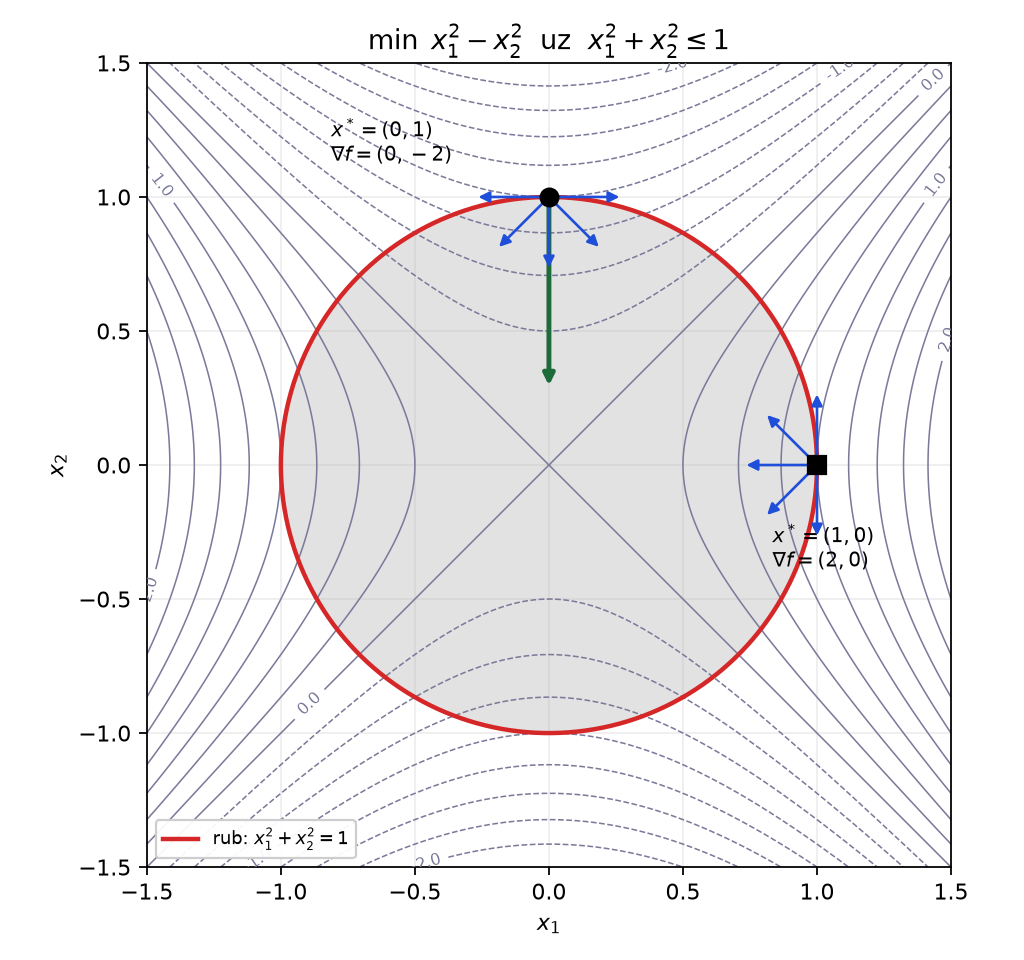
\includegraphics[width=0.72\textwidth]{03-sedlo-disk.png}
\caption{Sedlasta funkcija na jediničnom disku. U točki $(0,1)$ (krug)
gradijent (zeleno) pokazuje u disk, a svi dozvoljeni smjerovi (plavo) zatvaraju
s njim kut $\le 90^\circ$ --- uvjet je zadovoljen. U točki $(1,0)$ (kvadrat)
gradijent pokazuje van, a dozvoljeni smjerovi su mu suprotni --- uvjet je
prekršen.}
\end{figure}

% =====================================================================
\section{Problem s jednim ograničenjem jednakosti}
\label{sec:jedna-jednakost}
\str{19--32}

\subsection{Postavka}
\str{19}

\begin{equation}
\begin{aligned}
\min \quad & f(x) := x_1 + x_2 \\
\uzogr & h(x) := 2 - x_1^2 - x_2^2 = 0
\end{aligned}
\end{equation}

\textbf{Grafičkom metodom:} rješenje (minimizator) je $x^{*} = (-1, -1)$.

\textbf{Pitanje sa slajda:} \emph{Kako sistematski karakterizirati optimalna
rješenja?} --- odnosno, kako doći do rješenja bez crtanja?

\begin{napomena}[predznak funkcije $h$]
Na slajdu 19 je $h(x) = 2 - x_1^2 - x_2^2$, a već na sljedećem slajdu 20 piše
$\Feas = \{x \mid h(x) = x_1^2 + x_2^2 - 2 = 0\}$ --- dakle s obrnutim
predznakom. To \textbf{nije greška}: slajd 25 izričito kaže da je smjer normale
proizvoljan jer je $h(x) = 0$ ekvivalentno $-h(x) = 0$. Promjena predznaka mijenja
samo \emph{predznak} multiplikatora $\lambda$, ne i rješenje $x^{*}$. U ovoj
skripti slijedimo predznak sa slajda koji citiramo, i svaki put ga naznačimo.
\end{napomena}

\subsection{Izvod uvjeta}
\str{20--22}

Dozvoljeni skup: $\Feas = \{\, x \mid h(x) = x_1^2 + x_2^2 - 2 = 0 \,\}$.

U točki $x \in \Feas$, ako je $d$ dozvoljeni smjer sa smanjenjem funkcije cilja,
treba vrijediti:
\begin{align}
f(x + d) &\approx f(x) + \nabla f(x)\T d < f(x), \\
h(x + d) &\approx h(x) + \nabla h(x)\T d = 0,
\end{align}

\textbf{Odakle te dvije relacije.} Obje su \textbf{linearizacije}
(aproksimacija prvog reda, odjeljak~\ref{sec:gradijent}) za mali pomak $d$:

\begin{itemize}
  \item Prva: želimo da nova vrijednost cilja bude manja od stare.
  \item Druga: želimo ostati na krivulji ograničenja, dakle nova vrijednost
        $h$ mora i dalje biti nula.
\end{itemize}

\textbf{Pojednostavljenje} \str{21}\textbf{.} Takvi smjerovi $d$
okarakterizirani su sljedećim svojstvima:
\[
\nabla f(x)\T d < 0 \qquad\text{i}\qquad \nabla h(x)\T d = 0
\]

\emph{Raspis prve:} iz $f(x) + \nabla f(x)\T d < f(x)$ oduzmemo $f(x)$ s obje
strane $\Rightarrow$ $\nabla f(x)\T d < 0$.

\emph{Raspis druge:} budući da je $x$ već dopustiv, vrijedi $h(x) = 0$, pa iz
$h(x) + \nabla h(x)\T d = 0$ ostaje $\nabla h(x)\T d = 0$.

\textbf{Zaključak} \str{22}\textbf{.} U točki $x \in \Feas$ skup svih
dozvoljenih smjerova sa smanjenjem funkcije cilja je skup $P(x)$, gdje je
\[
P(x) = D(x) \cap S(x).
\]

\subsection{Geometrijska slika}
\str{23--26}

Slajdovi 23--26 grade jedan crtež u četiri koraka. Prikazana je kružnica
$x_1^2+x_2^2 = 2$ (dozvoljeni skup), preko nje kose paralelne nivo krivulje
funkcije $f = x_1+x_2$, i tri vrste strelica u točkama duž kružnice:

\begin{center}
\begin{tabular}{p{2.4cm}p{10.6cm}}
\toprule
\textbf{Boja} & \textbf{Značenje (doslovno sa slajdova)} \\
\midrule
\textcolor{zelena}{\textbf{zelene}} & $-\nabla f(x)$ \str{23} \\
\textcolor{fsbcrvena}{\textbf{crvene}} & $\nabla h(x)$; \emph{normale (okomice)
  na krivulju ograničenja dane su s $\nabla h(x)$} \str{24}. Smjer normale na
  krivulju ograničenja jednakosti može se uzeti \textbf{proizvoljan} jer je
  $h(x) = 0$ ekvivalentno $-h(x) = 0$ \str{25} \\
\textcolor{tamnoplava}{\textbf{plave}} & dozvoljeni smjerovi $d$ $=$ okomice na
  normale $\nabla h(x)$, tj.\ $\nabla h(x)\T d = 0$ \str{26} \\
\bottomrule
\end{tabular}
\end{center}

\textbf{Kako čitati sliku.} Zelene strelice pokazuju kamo bismo \emph{htjeli}
ići (smjer najbržeg pada cilja); one su svugdje jednake, jer je $\nabla f$
konstantan. Plave strelice pokazuju kamo \emph{smijemo} ići (tangencijalno na
kružnicu). U većini točaka zelena ima komponentu duž plave --- tada se pomakom
po kružnici cilj popravlja, pa ta točka nije optimum. Samo tamo gdje je zelena
strelica \textbf{potpuno okomita} na plave (dakle kolinearna s crvenom) nema
poboljšanja.

\begin{figure}[H]
\centering
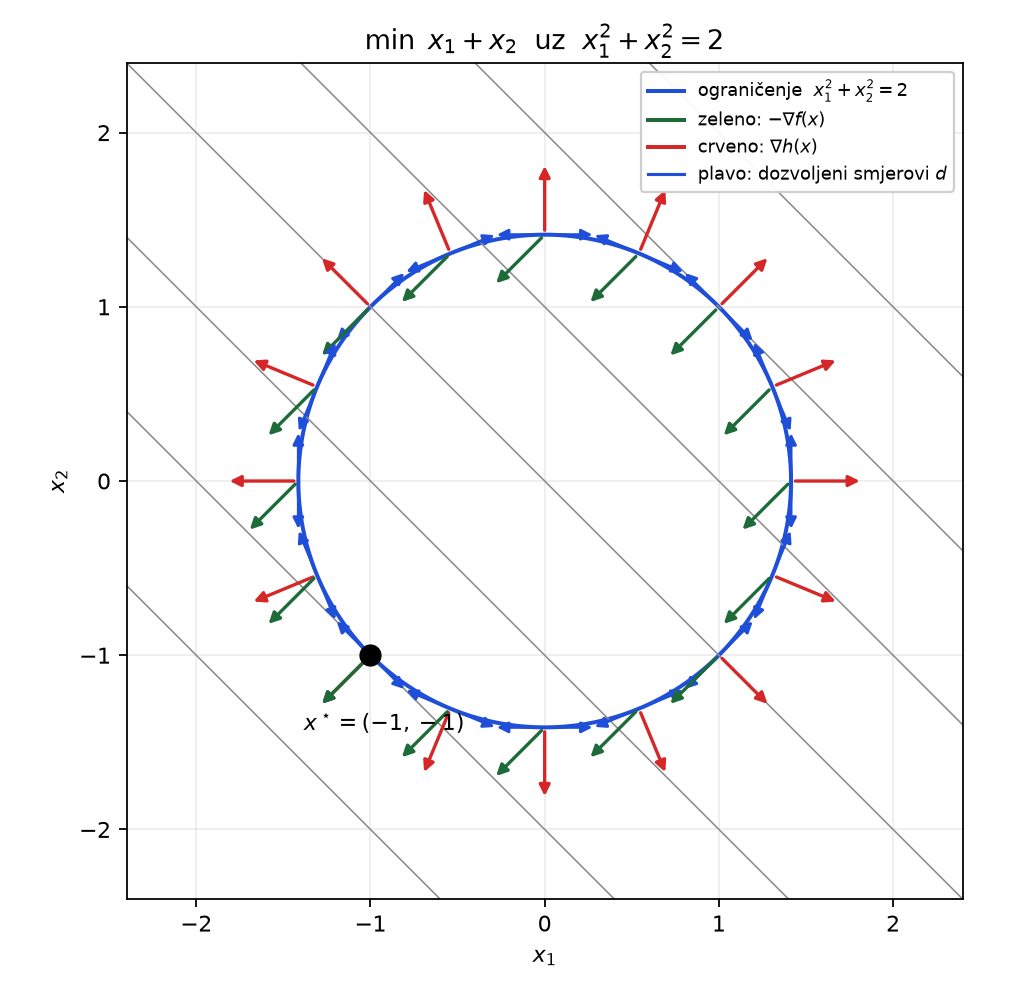
\includegraphics[width=0.74\textwidth]{03-jednakost-krug.png}
\caption{Rekonstrukcija crteža sa slajda 26. U optimumu $x^\star=(-1,-1)$
zelena strelica $-\nabla f$ poklapa se sa smjerom crvene $\nabla h$, pa nijedan
plavi (dozvoljeni) smjer ne smanjuje cilj.}
\end{figure}

\subsection{Uvjet kolinearnosti gradijenata}
\str{27--31}

\textbf{Kandidati za minimizatore} \str{27}\textbf{:} za svaki $d$ tako da je
$\nabla h(x)\T d = 0$, vrijedi $\nabla f(x)\T d = 0$.

\emph{Zašto baš to:} ako bi za neki dozvoljeni $d$ bilo $\nabla f\T d \ne 0$,
onda bi ili $d$ ili $-d$ (također dozvoljen, jer je i za njega
$\nabla h\T(-d) = 0$) dao $\nabla f\T d < 0$, tj.\ pad cilja. Dakle nužno je
$\nabla f\T d = 0$ za sve dozvoljene $d$.

\textbf{Ključni korak} \str{29}\textbf{.} Promotrimo slučaj kada je
\[
\nabla f(x) = \lambda \nabla h(x)
\]
za neku vrijednost $\lambda \in \R$ (dakle, kad su $\nabla f(x)$ i
$\nabla h(x)$ \textbf{kolinearni}).

\begin{napomena}[kolinearni]
Dva vektora su \textbf{kolinearna} (paralelna) ako je jedan skalarni višekratnik
drugoga. Geometrijski leže na istom pravcu; mogu pokazivati u isti smjer
($\lambda > 0$) ili u suprotan ($\lambda < 0$).
\end{napomena}

\textbf{Tada vrijedi} \str{30}:
\[
\big(\nabla f(x)\T - \lambda\nabla h(x)\T\big)d
= \nabla f(x)\T d - \lambda\nabla h(x)\T d = 0
\]
što znači da za svaki $d$ kad je $\nabla h(x)\T d = 0$ tada vrijedi i da je
$\nabla f(x)\T d = 0$.

\emph{Raspis:} lijeva zagrada je nula po pretpostavci kolinearnosti, pa je i
cijeli umnožak nula. Drugi član $\lambda\nabla h(x)\T d$ je također nula (jer je
$d$ dozvoljen). Iz $\nabla f\T d - 0 = 0$ slijedi $\nabla f\T d = 0$.
\checkmark

\begin{teorem}[Nužan uvjet za optimum --- jedno ograničenje jednakosti \str{31}]
Neka je $x^{*}$ lokalni minimizator. Tada vrijedi
\[
\nabla f(x^{*}) = \lambda\nabla h(x^{*}) \qquad\text{za neki } \lambda \in \R.
\]
\end{teorem}

\textbf{Riječima:} u optimumu gradijent funkcije cilja mora biti \textbf{paralelan}
gradijentu ograničenja. To je algebarski zapis onoga što smo očitali sa slike:
nivo krivulja cilja \emph{dodiruje} (a ne siječe) krivulju ograničenja.

\subsection{Provjera na primjeru}
\str{32}

Za naš primjer vrijedi:
\[
\nabla f(x) = \begin{pmatrix} 1 \\ 1 \end{pmatrix}, \qquad
\nabla h(x) = \begin{pmatrix} -2x_1 \\ -2x_2 \end{pmatrix}.
\]

\emph{Raspis:} $f = x_1 + x_2$ daje $\partial f/\partial x_1 = 1$,
$\partial f/\partial x_2 = 1$. Za $h = 2 - x_1^2 - x_2^2$ (predznak sa slajda
19) je $\partial h/\partial x_1 = -2x_1$, $\partial h/\partial x_2 = -2x_2$.
\checkmark

Za $x^{*} = (-1, -1)$ tada imamo
\[
\begin{pmatrix} 1 \\ 1 \end{pmatrix}
= \lambda^{*}\begin{pmatrix} 2 \\ 2 \end{pmatrix},
\qquad\text{što vrijedi za } \lambda^{*} = \tfrac{1}{2}.
\]

\emph{Uvrštavanje:} $\nabla h(-1,-1) = (-2\cdot(-1),\, -2\cdot(-1)) = (2, 2)$.
Iz $1 = 2\lambda^{*}$ slijedi $\lambda^{*} = 1/2$. Ista vrijednost izlazi i iz
druge komponente --- što je dobar znak: da su komponente dale različite
$\lambda$, vektori ne bi bili kolinearni. \checkmark

\begin{napomena}[ključno upozorenje sa slajda 32]
\textbf{Gornji uvjet je nužan ali ne i dovoljan!} I za točku $x = (1,1)$ imamo
da je $\nabla f(x) = \lambda\nabla h(x)$, ali \textbf{to nije optimalna točka}.

\emph{Provjera:} $\nabla h(1,1) = (-2,-2)$, pa iz $(1,1) = \lambda(-2,-2)$
slijedi $\lambda = -1/2$. Uvjet je zadovoljen. Ali $f(1,1) = 2$, dok je
$f(-1,-1) = -2$ --- točka $(1,1)$ je zapravo \textbf{maksimum} na kružnici.

\textbf{Pouka:} uvjet kolinearnosti hvata \emph{sve} stacionarne točke na
ograničenju --- i minimume i maksimume. Nakon rješavanja uvijek treba usporediti
vrijednosti $f$ u svim kandidatima.
\end{napomena}

% =====================================================================
\section{Lagrangeova funkcija}
\label{sec:lagrange}
\str{33--34}

Uvjet kolinearnosti je koristan, ali nezgodan za rješavanje. Sljedeći alat
pakira sve nužne uvjete u jednu funkciju.

\textbf{Problem} \str{33}:
\begin{equation}
\label{eq:zvj}
\min f(x) \quad\text{uz ograničenje}\quad h(x) = 0
\tag{$*$}
\end{equation}

\begin{definicija}[Lagrangeova funkcija]
Lagrangeova funkcija za optimizacijski problem \eqref{eq:zvj} definirana je na
sljedeći način:
\[
L(x, \lambda) = f(x) + \lambda h(x)
\]
\end{definicija}

\textbf{Zašto je Lagrangeova funkcija korisna?} \str{34} Ako je $x^{*}$ lokalni
minimizator, tada vrijedi
\begin{align}
\nabla_x L(x^{*}, \lambda^{*})
  &= \nabla f(x^{*}) + \lambda^{*}\nabla h(x^{*}) = 0
  \qquad\text{za neki } \lambda^{*} \\
\nabla_\lambda L(x^{*}, \lambda^{*}) &= h(x^{*}) = 0
\end{align}

\textbf{Dakle, nužni uvjeti za optimalnost mogu se izvesti iz Lagrangeove
funkcije.}

\textbf{Objašnjenje.}
\begin{itemize}
  \item $\nabla_x L$ znači „gradijent po varijablama $x$, uz $\lambda$ fiksan”.
        Analogno $\nabla_\lambda L$ je derivacija po $\lambda$, uz $x$ fiksan.
  \item Derivacija po $\lambda$ vraća točno $h(x)$, jer je $L$ linearna u
        $\lambda$: $\partial(\lambda h(x))/\partial\lambda = h(x)$. Time uvjet
        $\nabla_\lambda L = 0$ \emph{automatski} ponovno nameće ograničenje.
  \item \textbf{Genijalnost trika:} problem \emph{s} ograničenjem sveden je na
        traženje stacionarne točke jedne funkcije \emph{bez} ograničenja ---
        samo u prostoru veće dimenzije ($x$ \emph{i} $\lambda$).
\end{itemize}

\begin{napomena}[predznak $\lambda$: slajd 31 vs.\ slajd 34]
Na slajdu 31 uvjet glasi $\nabla f = \lambda\nabla h$, a iz Lagrangeove funkcije
na slajdu 34 dobiva se $\nabla f + \lambda\nabla h = 0$, tj.\
$\nabla f = -\lambda\nabla h$. \textbf{Radi se o istom uvjetu} --- razlikuje se
samo \emph{predznak} multiplikatora ($\lambda_{\text{sl.34}} =
-\lambda_{\text{sl.31}}$).

Za ograničenja \emph{jednakosti} to je potpuno nevažno, jer $\lambda$ smije biti
bilo kojeg predznaka. Kod ograničenja \emph{nejednakosti} predznak je bitan
(vidi uvjet $\mu \ge 0$ u odjeljku~\ref{sec:nejednakost}), pa se ondje
konzistentno koristi zapis s $+$, tj.\ $\nabla f + \mu\nabla g = 0$.
\end{napomena}

% =====================================================================
\section{Više ograničenja jednakosti}
\label{sec:vise-jednakosti}
\str{35--40}

\textbf{Problem} \str{35}:
\begin{equation}
\label{eq:zvj2}
\min f(x) \quad\text{uz ograničenja}\quad h_i(x) = 0,\; i = 1\dots m
\tag{$*$}
\end{equation}

\subsection{Regularna točka}
\str{35}

\begin{definicija}[Regularna točka kod ograničenja jednakosti]
Točka $x^{*}$ koja ispunjava uvjete $h_i(x^{*}) = 0$, $i = 1,\dots,m$ je
\textbf{regularna točka} ako su gradijenti $\nabla h_i(x^{*})$ \textbf{linearno
nezavisni}.
\end{definicija}

\textbf{Objašnjenje sa slajda:} dakle, ako je točka $x^{*}$ regularna točka,
tada nema paralelnih gradijenata $\nabla h_i(x^{*})$, niti nema gradijenata koji
se mogu izraziti kao \textbf{linearna kombinacija} ostalih gradijenata.

\begin{napomena}[linearna nezavisnost --- od nule]
Vektori $v_1,\dots,v_k$ su \textbf{linearno nezavisni} ako se nijedan od njih ne
može napisati kao kombinacija ostalih; formalno, ako iz
$c_1v_1 + \dots + c_kv_k = 0$ nužno slijedi $c_1 = \dots = c_k = 0$.

\emph{Zašto nam to treba:} ako su gradijenti ograničenja zavisni, ograničenja se
u toj točki „preklapaju” i geometrija degenerira --- uvjeti optimalnosti tada
mogu zakazati. Slajd 57 pokazuje upravo takav protuprimjer.
\end{napomena}

\subsection{Lagrangeova funkcija i nužni uvjeti}
\str{36--37}

\begin{definicija}[Lagrangeova funkcija, više jednakosti \str{36}]
\[
L(x, \lambda) = f(x) + \sum_{i=1}^{m}\lambda_i h_i(x)
\]
$\lambda_1, \lambda_2, \dots, \lambda_m$ zovu se \textbf{Lagrangeovi
množitelji}.
\end{definicija}

Uz uvjet da je $x$ \textbf{regularna točka}, nužni uvjeti za optimalnost tada
glase \str{36}:
\begin{align}
\frac{\partial L(x,\lambda)}{\partial x_i}
  &= \frac{\partial f(x)}{\partial x_i}
   + \sum_{j=1}^{m}\lambda_j\frac{\partial h_j(x)}{\partial x_i} = 0,
  && i = 1,\dots,n \\
\frac{\partial L(x,\lambda)}{\partial \lambda_i}
  &= h_i(x) = 0, && i = 1,\dots,m
\end{align}

\textbf{Kompaktniji zapis} \str{37}\textbf{.} Za problem \eqref{eq:zvj2}, ako je
$x$ regularna točka, nužni uvjeti za optimalnost mogu se zapisati u sljedećem
obliku:
\begin{align}
h_i(x) &= 0, && i = 1,\dots,m \\
\nabla f(x) + \sum_{i=1}^{m}\lambda_i\nabla h_i(x) &= 0
\end{align}

\textbf{Geometrijska interpretacija} \str{37--38}\textbf{:} u točki optimuma
$x^{*}$, vektor $\nabla f(x^{*})$ je \textbf{linearna kombinacija} gradijenata
funkcija ograničenja $\nabla h_i(x^{*})$ u toj točki.

To je poopćenje uvjeta kolinearnosti: s jednim ograničenjem $\nabla f$ je morao
biti \emph{paralelan} s $\nabla h$; s više ograničenja mora ležati u
\emph{ravnini} (općenito potprostoru) koju razapinju gradijenti ograničenja.

\subsection{Postupak traženja kandidata za optimum}
\str{39}

\begin{teorem}[Recept]
Iz nužnih uvjeta optimalnosti
\begin{align}
\frac{\partial L(x,\lambda)}{\partial x_i}
  &= \frac{\partial f(x)}{\partial x_i}
   + \sum_{j=1}^{m}\lambda_j\frac{\partial h_j(x)}{\partial x_i} = 0,
  && i = 1,\dots,n \\
\frac{\partial L(x,\lambda)}{\partial \lambda_i}
  &= h_i(x) = 0, && i = 1,\dots,m
\end{align}
odredimo $m + n$ nepoznanica $x_1,\dots,x_n,\ \lambda_1,\dots,\lambda_m$.

Na ovaj način dobivamo točke kandidate za minimizatora. \textbf{(Ovo su samo
nužni ali ne i dovoljni uvjeti!)}
\end{teorem}

\textbf{Zašto se brojevi poklapaju:} imamo $n$ jednadžbi iz derivacija po $x$ i
$m$ jednadžbi iz derivacija po $\lambda$ --- ukupno $n+m$ jednadžbi za $n+m$
nepoznanica. Sustav je time (općenito) određen.

\subsection{Primjer: paralelepiped najvećeg volumena upisan u kuglu}
\str{40}

\textbf{Zadatak (doslovno sa slajda).} Odrediti paralelepiped maksimalnog
volumena koji je sadržan u kugli polumjera $r$. Ishodište je u središtu kugle, a
vrhovi paralelepipeda su na površini kugle.

\textbf{Postavka geometrije (sa skice na slajdu).} Paralelepiped je postavljen
simetrično oko ishodišta, sa stranicama paralelnim osima. Ako je jedan njegov
vrh u točki $(x_1, x_2, x_3)$ (prvi oktant), onda su bridovi
\[
a = 2x_1, \qquad b = 2x_2, \qquad c = 2x_3
\]

\textbf{Funkcija cilja:}
\[
V = F(x) = 8x_1x_2x_3
\]

\emph{Odakle:} volumen kvadra je $a\cdot b\cdot c = 2x_1 \cdot 2x_2 \cdot 2x_3
= 8x_1x_2x_3$. \checkmark

\textbf{Nametnuta veza (ograničenje):}
\[
h(x) = x_1^2 + x_2^2 + x_3^2 - r^2 = 0
\]

\emph{Odakle:} vrh leži \emph{na} sferi polumjera $r$, a udaljenost vrha od
ishodišta je $\sqrt{x_1^2+x_2^2+x_3^2}$; izjednačena s $r$ i kvadrirana daje
gornji izraz.

\textbf{Lagrangeova funkcija:}
\[
L(x,\lambda) = 8x_1x_2x_3 + \lambda\big(x_1^2 + x_2^2 + x_3^2 - r^2\big)
\]

\textbf{Slijedi (sa slajda):}
\[
\begin{aligned}
\frac{\partial L}{\partial x_1} &= 8x_2x_3 + 2\lambda x_1 = 0
  &&\big/\;\cdot\, x_1 \\
\frac{\partial L}{\partial x_2} &= 8x_1x_3 + 2\lambda x_2 = 0
  &&\big/\;\cdot\, x_2 \\
\frac{\partial L}{\partial x_3} &= 8x_1x_2 + 2\lambda x_3 = 0
  &&\big/\;\cdot\, x_3
\end{aligned}
\qquad (+)
\]

\emph{Provjera derivacija:} u $8x_1x_2x_3$ derivacija po $x_1$ je $8x_2x_3$
(ostale varijable su konstante); u $\lambda(x_1^2+\dots)$ derivacija po $x_1$ je
$2\lambda x_1$. \checkmark

\textbf{Trik sa slajda:} svaka jednadžba se pomnoži naznačenom varijablom, pa se
sve tri \textbf{zbroje} (oznaka $(+)$):
\[
24x_1x_2x_3 + 2\lambda\big(x_1^2 + x_2^2 + x_3^2\big) = 0
\;\Longrightarrow\;
\lambda = -\frac{24x_1x_2x_3}{2r^2} = -\frac{3V}{2r^2}
\]

\emph{Raspis zbrajanja:}
\begin{align}
x_1 \cdot (8x_2x_3 + 2\lambda x_1) &= 8x_1x_2x_3 + 2\lambda x_1^2 = 0 \\
x_2 \cdot (8x_1x_3 + 2\lambda x_2) &= 8x_1x_2x_3 + 2\lambda x_2^2 = 0 \\
x_3 \cdot (8x_1x_2 + 2\lambda x_3) &= 8x_1x_2x_3 + 2\lambda x_3^2 = 0
\end{align}
Zbroj: $3\cdot 8x_1x_2x_3 + 2\lambda(x_1^2+x_2^2+x_3^2) = 0$, tj.\
$24x_1x_2x_3 + 2\lambda(x_1^2+x_2^2+x_3^2) = 0$. \checkmark

\emph{Zatim} se iskoristi ograničenje $x_1^2+x_2^2+x_3^2 = r^2$:
\[
24x_1x_2x_3 + 2\lambda r^2 = 0
\;\Longrightarrow\;
\lambda = -\frac{24x_1x_2x_3}{2r^2}
\]
i uz $V = 8x_1x_2x_3$, brojnik je $3V$, pa je $\lambda = -\dfrac{3V}{2r^2}$.
\checkmark

\textbf{Uvrštenjem $\lambda$ u $\partial L/\partial x_1$ slijedi:}
\[
8x_2x_3\left(1 - \frac{3x_1^2}{r^2}\right) = 0
\;\Longrightarrow\;
x_1 = \pm\frac{r}{\sqrt3} = \frac{r}{\sqrt3},
\quad\text{i analogno: } x_2 = x_3 = \frac{r}{\sqrt3}
\]

\emph{Raspis uvrštavanja:}
\begin{align}
8x_2x_3 + 2\lambda x_1
&= 8x_2x_3 + 2\left(-\frac{24x_1x_2x_3}{2r^2}\right)x_1 \\
&= 8x_2x_3 - \frac{24x_1^2x_2x_3}{r^2} \\
&= 8x_2x_3\left(1 - \frac{3x_1^2}{r^2}\right)
\end{align}
Umnožak je nula ako je $x_2x_3 = 0$ (odbačeno --- tada je volumen nula) ili ako
je zagrada nula:
\[
1 = \frac{3x_1^2}{r^2} \;\Longrightarrow\; x_1^2 = \frac{r^2}{3}
\;\Longrightarrow\; x_1 = \pm\frac{r}{\sqrt3}
\]
Uzimamo pozitivni korijen jer je vrh u prvom oktantu. \checkmark

\textbf{Volumen:}
\[
V_{\max} = \left(\frac{2r}{\sqrt3}\right)^{3}
\]

\emph{Provjera:} brid je $a = 2x_1 = 2r/\sqrt3$; ista vrijednost za $b$ i $c$,
pa je $V = a^3 = (2r/\sqrt3)^3 = \dfrac{8r^3}{3\sqrt3}$. \checkmark

\textbf{Zaključak:} optimalan paralelepiped je \textbf{kocka}. To je tipičan
ishod simetričnih problema --- i lijep primjer kako Lagrangeova metoda riješi u
tri retka ono što bi eliminacijom varijabli bilo mnogo dulje.

\begin{napomena}[maksimizacija Lagrangeovom metodom]
Ovaj je zadatak \emph{maksimizacija}, a nužni uvjeti su izvedeni za
minimizaciju. To je u redu: uvjet $\nabla L = 0$ hvata \emph{sve} stacionarne
točke --- i minimume i maksimume (usporedi napomenu uz slajd 32). Da je trebalo
formalno slijediti standardnu formu, minimizirali bismo $-V$
(trik iz odjeljka~\ref{sec:trikovi}); rješenje $x^\star$ bilo bi isto, a
$\lambda$ bi promijenio predznak.
\end{napomena}

% =====================================================================
\section{Problem s jednim ograničenjem nejednakosti}
\label{sec:nejednakost}
\str{41--51}

\subsection{Postavka}
\str{41}

\begin{equation}
\begin{aligned}
\min \quad & f(x) := x_1 + x_2 \\
\uzogr & g(x) := x_1^2 + x_2^2 - 2 \le 0
\end{aligned}
\end{equation}

\textbf{Grafičkom metodom:} rješenje (minimizator) je $x^{*} = (-1,-1)$.

Uočite: isti cilj i isti rub kao u odjeljku~\ref{sec:jedna-jednakost}, ali
dozvoljeni skup je sada cijeli \textbf{disk} umjesto same kružnice. Rješenje je
ispalo isto --- ali sada moramo objasniti \emph{zašto} optimum leži baš na rubu.

\subsection{Izvod: dva slučaja}
\str{42--45}

Dozvoljeni skup: $\Feas = \{\, x \mid g(x) := x_1^2 + x_2^2 - 2 \le 0 \,\}$.

U točki $x \in \Feas$, ako je $d$ dozvoljeni smjer sa smanjenjem funkcije cilja,
treba vrijediti \str{42}:
\begin{align}
f(x+d) &\approx f(x) + \nabla f(x)\T d < f(x), \\
g(x+d) &\approx g(x) + \nabla g(x)\T d \le 0.
\end{align}

Razlika u odnosu na jednakost: druga relacija sada ima $\le 0$ umjesto $= 0$, i
$g(x)$ \textbf{ne} mora biti nula, pa se ne može jednostavno pokratiti. Zato
uvodimo novi pojam:

\begin{definicija}[Aktivno i neaktivno ograničenje \str{43}]
Neka je $x \in \R^n$. Kažemo da je ograničenje $g(x) \le 0$ \textbf{aktivno} u
$x$ ako vrijedi $g(x) = 0$. Ako pak vrijedi $g(x) < 0$, kažemo da je ograničenje
$g(x) \le 0$ \textbf{neaktivno} u $x$.
\end{definicija}

\textbf{Slikovito:} aktivno ograničenje znači „stojimo točno na ogradi”, a
neaktivno „ograda je negdje daleko, trenutno nas ne dodiruje”.

\textbf{Slajd 44--45 razlikuje dva slučaja:}

\textbf{1) Neaktivno ograničenje: $g(x) < 0$.}
$d$ je dozvoljen smjer sa smanjenjem funkcije cilja u $x$ ako vrijedi
\[
g(x) + \nabla g(x)\T d \le 0, \qquad \nabla f(x)\T d < 0
\]
što je, u slučaju kad je $\|d\|$ uzet dovoljno malen\footnote{Fusnota sa slajda:
za bilo koji smjer, uvjet $g(x) + \nabla g(x)\T d \le 0$ može se uvijek
zadovoljiti ako je duljina vektora $d$ dovoljno malena, jer je $g(x) < 0$.},
ekvivalentno uvjetu
\[
\nabla f(x)\T d < 0.
\]

\textbf{2) Aktivno ograničenje: $g(x) = 0$.}
$d$ je dozvoljen smjer sa smanjenjem funkcije cilja u $x$ ako vrijedi
\[
\nabla g(x)\T d \le 0, \qquad \nabla f(x)\T d < 0
\]

\emph{Zašto je u slučaju 2 nestao $g(x)$:} jer je $g(x) = 0$, pa uvjet
$g(x) + \nabla g(x)\T d \le 0$ postaje $\nabla g(x)\T d \le 0$.

\subsection{Nužni uvjeti za oba slučaja}
\str{46--48}

\textbf{Osnovna ideja} \str{46}\textbf{:} kandidati za optimum su one točke
$x^{*}$ za koje je skup dozvoljenih smjerova sa smanjenjem funkcije cilja
\textbf{prazan skup}.

\textbf{1) Neaktivno ograničenje u $x^{*}$: $g(x^{*}) < 0$.} Nužan uvjet za
optimum je
\[
\nabla f(x^{*}) = 0
\]
jer je jedino tada skup $\{\, d \mid \nabla f(x)\T d < 0 \,\}$ nužno prazan.

\emph{Zašto:} ako je $\nabla f \ne 0$, uvijek možemo uzeti $d = -\nabla f$ i
dobiti $\nabla f\T d = -\|\nabla f\|^2 < 0$ --- dakle smjer pada postoji.
Prazan skup dobivamo samo kad je gradijent nula. Ovo je zapravo poznati uvjet
za probleme \emph{bez} ograničenja --- logično, jer nas ograničenje ovdje ni ne
dodiruje.

\textbf{2) Aktivno ograničenje u $x^{*}$: $g(x^{*}) = 0$} \str{47}\textbf{.}
Nužan uvjet za optimum glasi: za sve $d$ za koje vrijedi
$\nabla g(x)\T d \le 0$, mora nužno vrijediti i da je $\nabla f(x)\T d \ge 0$. U
tom slučaju je naime skup dozvoljenih smjerova sa smanjenjem funkcije cilja
prazan skup.

\begin{napomena}[tipfeler na slajdu 47/48]
Na slajdovima piše „$\nabla f(x)\T \ge 0$”; nedostaje $d$. Iz konteksta i iz
izvoda na slajdu 48 jasno je da se misli na $\nabla f(x)\T d \ge 0$.
\end{napomena}

\textbf{Ključni korak} \str{48}\textbf{.} Promotrimo slučaj kad je
\begin{equation}
\label{eq:dvijezvj}
\nabla f(x^{*}) + \mu^{*}\nabla g(x^{*}) = 0 \qquad\text{za neki }
\mu^{*} \ge 0
\tag{$**$}
\end{equation}

Tada vrijedi
\[
\big(\nabla f(x^{*})\T + \mu^{*}\nabla g(x^{*})\T\big)d = 0
\qquad\text{odnosno}\qquad
\nabla f(x^{*})\T d = -\mu^{*}\nabla g(x^{*})\T d
\]

Dakle, za sve $d$ za koje je $\nabla g(x^{*})\T d \le 0$, u tom slučaju nužno
vrijedi da je $\nabla f(x^{*})\T d \ge 0$.

\emph{Raspis zadnjeg zaključka --- pazite na dva predznaka:}
\begin{itemize}
  \item $\nabla g(x^{*})\T d \le 0$ (pretpostavka: $d$ je dozvoljen),
  \item $\mu^{*} \ge 0$ (pretpostavka),
  \item dakle $\mu^{*}\nabla g(x^{*})\T d \le 0$ (nenegativan puta nepozitivan),
  \item dakle $-\mu^{*}\nabla g(x^{*})\T d \ge 0$ (množenje s $-1$ okreće),
  \item a to je upravo $\nabla f(x^{*})\T d$. \checkmark
\end{itemize}

\textbf{Zaključak sa slajda:} uvjet \eqref{eq:dvijezvj} je nužan uvjet da bi
skup dozvoljenih smjerova sa smanjenjem funkcije cilja bio prazan skup.

\begin{napomena}[zašto baš $\mu \ge 0$, a $\lambda$ smije biti bilo koji]
Kod \emph{jednakosti} dozvoljeni smjerovi zadovoljavaju $\nabla h\T d = 0$ ---
simetrično, pa je predznak $\lambda$ nevažan.

Kod \emph{nejednakosti} dozvoljeni smjerovi zadovoljavaju $\nabla g\T d \le 0$
--- \emph{nesimetrično}. Gornji izvod prolazi samo ako je $\mu^{*} \ge 0$; s
negativnim $\mu^{*}$ zaključak bi se okrenuo. Geometrijski: $-\nabla f$ mora
pokazivati \emph{van} iz dozvoljenog skupa, u istom smjeru kao $\nabla g$.
\end{napomena}

\subsection{Teorem: uvjeti za jedno ograničenje nejednakosti}
\str{49--50}

\begin{teorem}[Nužni uvjeti, jedno ograničenje nejednakosti]
Za problem $\min f(x)$ uz ograničenje $g(x) \le 0$: ako je $x^{*}$ lokalni
minimizator, tada postoji $\mu^{*}$ tako da su sljedeći uvjeti zadovoljeni:
\begin{align}
\nabla f(x^{*}) + \mu^{*}\nabla g(x^{*}) &= 0 &&\text{(A1)} \\
\mu^{*}g(x^{*}) &= 0 &&\text{(A2)} \\
\mu^{*} &\ge 0 &&\text{(A3)}
\end{align}
\end{teorem}

\textbf{Kako teorem pokriva oba slučaja} \str{50}\textbf{.} Uočimo da je:

\begin{itemize}
  \item za $g(x^{*}) < 0$ (neaktivno), zbog (A2) imamo da je $\mu^{*} = 0$, pa
        (A1) postaje $\nabla f(x^{*}) = 0$;
  \item za $g(x^{*}) = 0$ (aktivno), slijedi da je $\mu^{*} \ge 0$ i
        $\nabla f(x^{*}) + \mu^{*}\nabla g(x^{*}) = 0$;
\end{itemize}

pa gornji teorem uključuje i slučaj aktivnog i slučaj neaktivnog ograničenja.

\begin{definicija}[Uvjet komplementarnosti \str{50}]
Uvjet (A2), $\mu^{*}g(x^{*}) = 0$, zove se \textbf{uvjet komplementarnosti}
(engl.\ \emph{complementary slackness}).
\end{definicija}

\textbf{Kako čitati uvjet komplementarnosti.} Umnožak dvaju brojeva je nula samo
ako je barem jedan od njih nula. Dakle u optimumu za svako ograničenje vrijedi
\textbf{barem jedno} od:
\begin{itemize}
  \item $\mu^{*} = 0$ --- ograničenje je „bez cijene”, ne utječe na rješenje;
  \item $g(x^{*}) = 0$ --- ograničenje je aktivno, „stojimo na ogradi”.
\end{itemize}
Ne mogu istovremeno biti $\mu^{*} > 0$ \emph{i} $g(x^{*}) < 0$. Ovo je
\emph{najkorisniji} uvjet u praksi: on nam govori koje kombinacije aktivnih
ograničenja uopće trebamo isprobavati.

\subsection{Zapis preko Lagrangeove funkcije}
\str{51}

\begin{definicija}[Lagrangeova funkcija za nejednakost]
Za problem $\min f(x)$ uz $g(x)\le 0$:
\[
L(x,\mu) = f(x) + \mu g(x)
\]
\end{definicija}

Ako je $x^{*}$ lokalni minimizator, tada vrijedi:
\begin{align}
\nabla_x L(x^{*},\mu^{*}) &= \nabla f(x^{*}) + \mu^{*}\nabla g(x^{*}) = 0 \\
g(x^{*}) &\le 0 \\
\mu^{*}g(x^{*}) &= 0 \\
\mu^{*} &\ge 0
\end{align}

\subsection{Rješavanje primjera sa slajda 41}

Slajd 41 daje rješenje grafički; ovdje ga izvodimo iz gornjih uvjeta, jer je to
postupak koji ćete koristiti na ispitu.

\textbf{Zadano:} $f(x) = x_1+x_2$, $g(x) = x_1^2+x_2^2-2 \le 0$.

\textbf{Gradijenti:}
\[
\nabla f(x) = \begin{pmatrix}1\\1\end{pmatrix}, \qquad
\nabla g(x) = \begin{pmatrix}2x_1\\2x_2\end{pmatrix}
\]

\textbf{Slučaj A --- ograničenje neaktivno} ($\mu^{*} = 0$). Tada (A1) traži
$\nabla f(x^{*}) = 0$, tj.\ $(1,1) = (0,0)$ --- \textbf{nemoguće}. Dakle
ograničenje mora biti aktivno.

\emph{Poanta:} to je algebarska potvrda geometrijske činjenice da linearna
funkcija nema unutarnji minimum --- uvijek se „gura” do ruba.

\textbf{Slučaj B --- ograničenje aktivno} ($g(x^{*}) = 0$). Sustav:
\begin{align}
1 + 2\mu^{*} x_1^{*} &= 0 \label{eq:kkt-b1}\\
1 + 2\mu^{*} x_2^{*} &= 0 \label{eq:kkt-b2}\\
(x_1^{*})^2 + (x_2^{*})^2 - 2 &= 0 \label{eq:kkt-b3}
\end{align}

\emph{Korak 1.} Iz \eqref{eq:kkt-b1} i \eqref{eq:kkt-b2} (uz $\mu^{*} \ne 0$,
što slijedi jer $\mu^{*}=0$ vodi na $1 = 0$):
\[
x_1^{*} = -\frac{1}{2\mu^{*}}, \qquad x_2^{*} = -\frac{1}{2\mu^{*}}
\]
dakle $x_1^{*} = x_2^{*}$.

\emph{Korak 2.} Uvrstimo u \eqref{eq:kkt-b3}:
\[
2(x_1^{*})^2 = 2 \;\Longrightarrow\; (x_1^{*})^2 = 1
\;\Longrightarrow\; x_1^{*} = \pm 1
\]

\emph{Korak 3 --- izbor predznaka pomoću (A3).} Iz
$x_1^{*} = -1/(2\mu^{*})$ i uvjeta $\mu^{*} \ge 0$ slijedi da $x_1^{*}$ mora
biti \textbf{negativan}. Dakle $x_1^{*} = x_2^{*} = -1$.

\emph{Korak 4 --- vrijednost multiplikatora.} Iz \eqref{eq:kkt-b1}:
\[
1 + 2\mu^{*}(-1) = 0 \;\Longrightarrow\; 2\mu^{*} = 1
\;\Longrightarrow\; \mu^{*} = \tfrac12 \ge 0 \quad\checkmark
\]

\textbf{Rezultat:}
\[
x^{*} = (-1,-1), \qquad \mu^{*} = \tfrac12, \qquad f(x^{*}) = -2
\]
što se poklapa s grafičkim rješenjem sa slajda 41. \checkmark

\begin{napomena}[usporedba s jednakošću]
U odjeljku~\ref{sec:jedna-jednakost} isti je problem s \emph{jednakošću} dao dvije
stacionarne točke: $(-1,-1)$ (minimum) i $(1,1)$ (maksimum). Ovdje je uvjet
$\mu \ge 0$ \textbf{sam odbacio} točku $(1,1)$. To je praktična prednost
nejednakosti: predznak multiplikatora nosi informaciju o smjeru, pa maksimumi
otpadaju automatski.
\end{napomena}

\begin{crtanje}[KKT točka na disku]
\textbf{Korak 1.} Nacrtajte osi $x_1, x_2$ od $-2{,}4$ do $2{,}4$, jednako
mjerilo.

\textbf{Korak 2 --- dozvoljeni skup.} Nacrtajte kružnicu polumjera
$\sqrt2 \approx 1{,}41$ oko ishodišta. Testna točka $(0,0)$ daje
$g = -2 \le 0$ \checkmark, dakle dopuštena je \textbf{unutrašnjost}; osjenčajte
je.

\textbf{Korak 3 --- nivo krivulje cilja.} $f = x_1+x_2 = c$ su paralelni pravci
nagiba $-1$. Nacrtajte ih za $c = -3, -2, -1, 0, 1, 2$. Označite ih; uočite da
$f$ pada kako se pomičemo prema \emph{dolje-lijevo}.

\textbf{Korak 4 --- optimum.} „Gurajte” pravac prema dolje-lijevo dok još
dodiruje disk. Zadnji dodir je u točki $(-1,-1)$; tu nacrtajte punu točku.
Provjera: $-1-1 = -2$, dakle taj pravac je $c = -2$.

\textbf{Korak 5 --- gradijent cilja.} Iz $(-1,-1)$ nacrtajte
$\nabla f = (1,1)$: jedna jedinica desno, jedna gore --- dakle prema
\emph{unutrašnjosti} diska. To je smjer rasta cilja.

\textbf{Korak 6 --- gradijent ograničenja.} Iz iste točke nacrtajte
$\nabla g = (2x_1, 2x_2) = (-2,-2)$: dvije jedinice lijevo, dvije dolje ---
dakle prema \emph{van} iz diska, okomito na kružnicu.

\textbf{Korak 7 --- provjera KKT-a okom.} Dvije strelice su
\textbf{antiparalelne} (leže na istom pravcu, suprotnih smjerova). Baš to
izražava (A1): $\nabla f = -\mu\nabla g$ uz $\mu = 1/2 > 0$. Duljina $\nabla f$
je upravo pola duljine $\nabla g$ --- odatle $\mu = 1/2$.

\textbf{Što graf znači.} U KKT točki nivo krivulja cilja \textbf{tangira} rub
dozvoljenog skupa, a gradijenti su antiparalelni. Da nisu, mogli bismo kliznuti
po rubu i smanjiti cilj. Uvjet $\mu \ge 0$ znači da $\nabla f$ pokazuje
\emph{unutra}: cilj bi rastao kad bismo se vratili u unutrašnjost, pa je
isplativo ostati priljubljen uz ogradu.
\end{crtanje}

\begin{figure}[H]
\centering
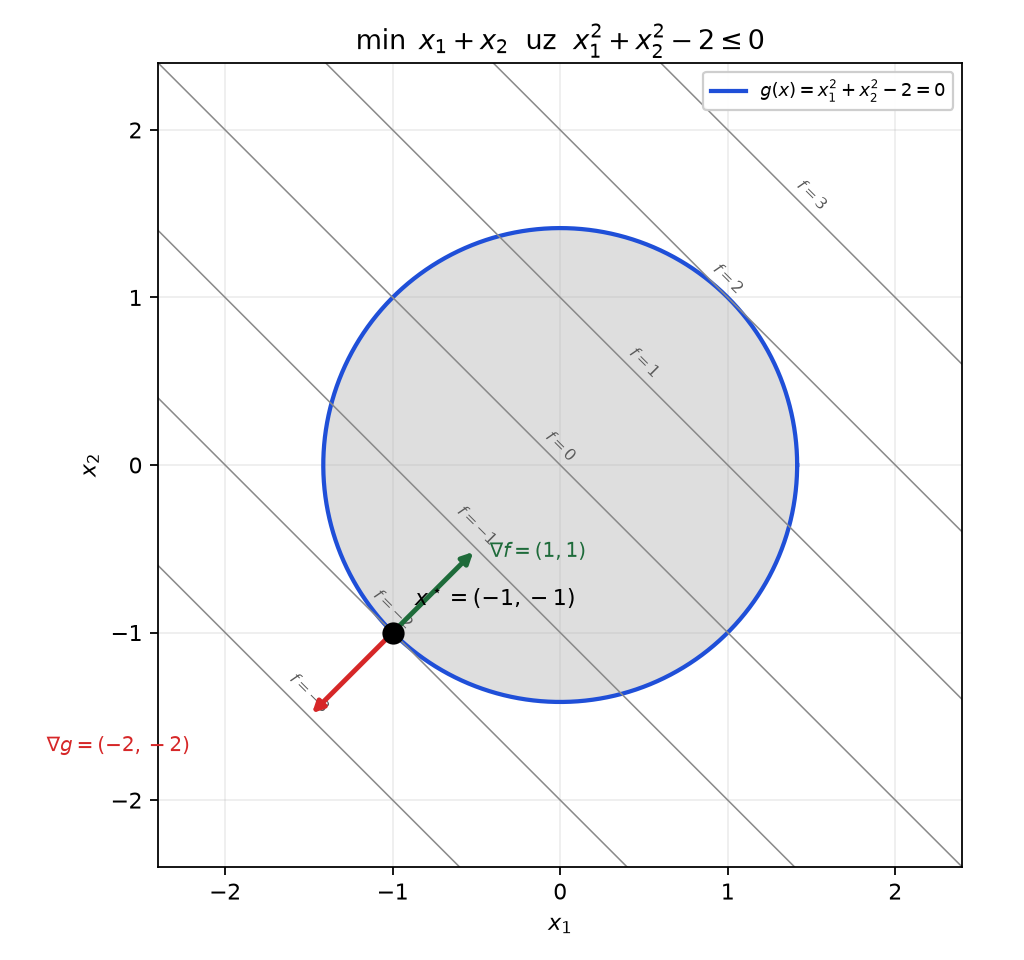
\includegraphics[width=0.70\textwidth]{03-nejednakost-krug.png}
\caption{KKT točka za $\min x_1+x_2$ uz $x_1^2+x_2^2 \le 2$. U $x^\star=(-1,-1)$
gradijenti $\nabla f$ (zeleno) i $\nabla g$ (crveno) su antiparalelni, uz
$\mu^{*}=\tfrac12 \ge 0$.}
\end{figure}

% =====================================================================
\section{Više ograničenja nejednakosti}
\str{52--57}

\textbf{Problem} \str{52}:
\begin{equation}
\label{eq:zvj3}
\min f(x) \quad\text{uz ograničenja}\quad g_i(x) \le 0,\; i = 1,\dots,p
\tag{$*$}
\end{equation}

\begin{definicija}[Lagrangeova funkcija \str{52}]
\[
L(x,\mu) = f(x) + \sum_{i=1}^{p}\mu_i g_i(x)
\]
Varijable $\mu = (\mu_1,\dots,\mu_p)$ zovu se \textbf{Lagrangeovi množitelji}.
\end{definicija}

\begin{definicija}[Regularna točka kod ograničenja nejednakosti \str{53}]
Neka je skup $I$ skup indeksa svih ograničenja koja su \textbf{aktivna} u točki
$x^{*}$, tj.\ neka je $I := \{\, i \mid g_i(x^{*}) = 0 \,\}$. Tada je $x^{*}$
\textbf{regularna točka} ako su gradijenti $\nabla g_i(x^{*})$ linearno
nezavisni za sve $i \in I$.
\end{definicija}

\textbf{Objašnjenje sa slajda:} dakle, ako je točka $x^{*}$ regularna točka, tada
među svim \emph{aktivnim} ograničenjima nema paralelnih gradijenata
$\nabla g_i(x^{*})$, niti nema gradijenata koji se mogu izraziti kao linearna
kombinacija gradijenata ostalih aktivnih ograničenja.

\begin{napomena}[samo aktivna ograničenja]
Uočite da se u definiciju regularnosti \textbf{uključuju samo aktivna}
ograničenja. Neaktivna ne igraju nikakvu ulogu --- ona ionako imaju $\mu_i = 0$
i lokalno ne dodiruju rješenje.
\end{napomena}

\begin{teorem}[Nužni uvjeti, više nejednakosti \str{54}]
Neka je $x^{*}$ regularna točka. Ako je $x^{*} \in \R^n$ lokalni minimizator,
tada postoji $\mu^{*} = (\mu_1^{*},\dots,\mu_p^{*})$ tako da su sljedeći uvjeti
zadovoljeni:
\begin{align}
\frac{\partial L}{\partial x_i}(x^{*},\mu^{*})
  &= \frac{\partial f}{\partial x_i}(x^{*})
   + \sum_{j=1}^{p}\mu_j^{*}\frac{\partial g_j}{\partial x_i}(x^{*}) = 0,
  && i = 1,\dots,n \\
g_j(x^{*}) &\le 0, && j = 1,\dots,p \\
\mu_j^{*}g_j(x^{*}) &= 0, && j = 1,\dots,p \\
\mu_j^{*} &\ge 0, && j = 1,\dots,p
\end{align}
\end{teorem}

\textbf{Kompaktniji zapis} \str{55}\textbf{.} Isti teorem, prva jednadžba
zapisana vektorski:
\begin{align}
\nabla f(x^{*}) + \sum_{j=1}^{p}\mu_j^{*}\nabla g_j(x^{*}) &= 0 \\
g_j(x^{*}) &\le 0, && j = 1,\dots,p \\
\mu_j^{*}g_j(x^{*}) &= 0, && j = 1,\dots,p \\
\mu_j^{*} &\ge 0, && j = 1,\dots,p
\end{align}

\subsection{Geometrijska interpretacija}
\str{56}

Slajd 56 prikazuje crtež u ravnini $(x_1, x_2)$:

\begin{itemize}
  \item dvije podebljane krivulje označene $g_1$ i $g_2$ --- granice dvaju
        ograničenja; ružičasto osjenčano područje između njih je dozvoljeni skup
        $S$;
  \item točka $x^{*}$ u kojoj se te dvije granice sijeku --- dakle \emph{oba}
        ograničenja su ondje aktivna;
  \item iz $x^{*}$ izlaze tri strelice: $\mu_1\nabla g_1$ (prema gore),
        $\mu_2\nabla g_2$ (prema gore-lijevo) i $\nabla F$ (prema dolje-desno);
  \item isprekidana krivulja $F(x^{*})$ --- nivo krivulja funkcije cilja kroz
        $x^{*}$, koja u toj točki dodiruje kut dozvoljenog skupa;
  \item zatvorena krivulja gore lijevo sa šrafiranom točkom u sredini ---
        neograničeni minimum cilja, koji leži izvan dozvoljenog skupa.
\end{itemize}

\textbf{Poruka slike:} $\nabla F$ je uravnotežen zbrojem $\mu_1\nabla g_1 +
\mu_2\nabla g_2$, uz $\mu_1,\mu_2 \ge 0$. Vektor $-\nabla F$ leži \emph{unutar
stošca} razapetog gradijentima aktivnih ograničenja. To je geometrijski sadržaj
prvog KKT uvjeta kad je aktivno više ograničenja.

\subsection{Važna iznimka: neregularna točka}
\str{57}

\textbf{Tvrdnja sa slajda:} \emph{Uvjeti optimalnosti ne moraju biti zadovoljeni
u neregularnoj točki.}

Slajd prikazuje sličan crtež, ali sada su u točki $x^{*}$ gradijenti
$\nabla g_1$ i $\nabla g_2$ \textbf{gotovo suprotni} (kolinearni), tj.\ linearno
zavisni --- dozvoljeni skup $S$ ima ondje „šiljak”. Vektor $\nabla F$ pokazuje
u smjeru koji se \emph{ne} može prikazati kao nenegativna kombinacija
$\nabla g_1$ i $\nabla g_2$.

\textbf{Zaključak:} $x^{*}$ jest optimum, ali KKT uvjeti u njemu \textbf{nemaju
rješenje}. Zato u svim teoremima stoji pretpostavka regularnosti.

\begin{napomena}[praktična važnost]
Pretpostavka regularnosti (u literaturi: \emph{constraint qualification}) u
praksi je gotovo uvijek ispunjena, pa se rijetko provjerava. Ali ako KKT sustav
nema rješenje, a znate da optimum postoji --- provjerite je li kandidatna točka
možda neregularna.
\end{napomena}

% =====================================================================
\section{KKT uvjeti: općenit slučaj}
\label{sec:kkt}
\str{58--61}

Sada spajamo sve: i jednakosti i nejednakosti.

\textbf{Optimizacijski problem} \str{58}:
\begin{equation}
\begin{aligned}
\minim & f(x) \\
\uzogr & h_i(x) = 0, && i = 1,\dots,m \\
       & g_j(x) \le 0, && j = 1,\dots,p
\end{aligned}
\end{equation}

\begin{definicija}[Regularna točka --- opći slučaj \str{58}]
Neka je $x^{*}$ točka koja zadovoljava sva ograničenja i neka je skup $J$ skup
indeksa svih ograničenja nejednakosti koja su aktivna u $x^{*}$, tj.\ neka je
$J := \{\, j \mid g_j(x^{*}) = 0 \,\}$. Tada je $x^{*}$ \textbf{regularna
točka} ako su gradijenti $\nabla h_i(x^{*})$, $i = 1,\dots,m$, i
$\nabla g_j(x^{*})$, $j \in J$, \textbf{linearno nezavisni}.
\end{definicija}

Dakle (sa slajda), ako je točka $x^{*}$ regularna točka, tada među svim
ograničenjima jednakosti i \emph{aktivnim} ograničenjima nejednakosti nema
paralelnih gradijenata niti gradijenata koji se mogu izraziti kao linearna
kombinacija ostalih gradijenata iz tog skupa.

\begin{teorem}[Karush-Kuhn-Tucker uvjeti \str{59}]
Neka je $x^{*}$ regularna točka. Ako je $x^{*} \in \R^n$ lokalni minimizator,
tada postoje Lagrangeovi množitelji $\lambda^{*} = (\lambda_1^{*},\dots,
\lambda_m^{*})$ i $\mu^{*} = (\mu_1^{*},\dots,\mu_p^{*})$ tako da su sljedeći
uvjeti zadovoljeni:
\begin{align}
\nabla f(x^{*}) + \sum_{i=1}^{m}\lambda_i^{*}\nabla h_i(x^{*})
  + \sum_{j=1}^{p}\mu_j^{*}\nabla g_j(x^{*}) &= 0
  &&\text{(stacionarnost)} \\
h_i(x^{*}) &= 0, && i = 1,\dots,m \\
g_j(x^{*}) &\le 0, && j = 1,\dots,p \\
\mu_j^{*}g_j(x^{*}) &= 0, && j = 1,\dots,p \\
\mu_j^{*} &\ge 0, && j = 1,\dots,p
\end{align}
Gornji uvjeti zovu se \textbf{Karush-Kuhn-Tucker nužni uvjeti optimalnosti} ili
skraćeno \textbf{KKT uvjeti}.
\end{teorem}

\textbf{Imena pojedinih skupina uvjeta} (standardna terminologija, korisna za
snalaženje u literaturi):

\begin{center}
\begin{tabular}{ll}
\toprule
\textbf{Uvjet} & \textbf{Naziv} \\
\midrule
$\nabla f + \sum\lambda_i\nabla h_i + \sum\mu_j\nabla g_j = 0$
  & stacionarnost ($\nabla_x L = 0$) \\
$h_i(x^{*}) = 0$, $g_j(x^{*}) \le 0$ & primarna dopustivost \\
$\mu_j^{*} \ge 0$ & dualna dopustivost \\
$\mu_j^{*}g_j(x^{*}) = 0$ & komplementarnost \\
\bottomrule
\end{tabular}
\end{center}

\begin{definicija}[Lagrangeova funkcija --- opći slučaj \str{60}]
\[
L(x,\lambda,\mu) = f(x) + \sum_{i=1}^{m}\lambda_ih_i(x)
                        + \sum_{i=1}^{p}\mu_ig_i(x)
\]
Varijable $\lambda = (\lambda_1,\dots,\lambda_m)$ i
$\mu = (\mu_1,\dots,\mu_p)$ zovu se \textbf{Lagrangeovi množitelji}.
\end{definicija}

\begin{napomena}[tipfeler na slajdu 60]
Na slajdu piše $\lambda = (\lambda_1,\dots,\lambda_p)$; treba biti
$(\lambda_1,\dots,\lambda_m)$, jer $\lambda$ pripada ograničenjima jednakosti
kojih ima $m$ (usporedi slajd 59).
\end{napomena}

\textbf{KKT uvjeti izraženi preko $L$} \str{61}\textbf{.} Slajd 61 ponavlja
teorem, ali svaki uvjet pridružuje odgovarajućoj derivaciji Lagrangeove
funkcije:
\begin{align}
\nabla_x L(x^{*},\lambda^{*},\mu^{*}) = 0
  &\;\Longrightarrow\; \nabla f(x^{*})
    + \sum_{i=1}^{m}\lambda_i^{*}\nabla h_i(x^{*})
    + \sum_{j=1}^{p}\mu_j^{*}\nabla g_j(x^{*}) = 0 \\
\nabla_\lambda L(x^{*},\lambda^{*},\mu^{*}) = 0
  &\;\Longrightarrow\; h_i(x^{*}) = 0, \quad i = 1,\dots,m \\
\nabla_\mu L(x^{*},\lambda^{*},\mu^{*}) \le 0
  &\;\Longrightarrow\; g_j(x^{*}) \le 0, \quad j = 1,\dots,p \\
&\phantom{\;\Longrightarrow\;} \mu_j^{*}g_j(x^{*}) = 0, \quad j = 1,\dots,p \\
&\phantom{\;\Longrightarrow\;} \mu_j^{*} \ge 0, \quad j = 1,\dots,p
\end{align}

\textbf{Praktični recept za rješavanje KKT sustava} (postupak koji slijedi iz
gornjih uvjeta i koji ćemo koristiti u poglavlju~\ref{ch:dualnost}):

\begin{enumerate}
  \item Napiši $L(x,\lambda,\mu)$.
  \item Izračunaj $\nabla_x L = 0$ --- to je $n$ jednadžbi.
  \item Dodaj sve jednakosti $h_i(x) = 0$ --- $m$ jednadžbi.
  \item \textbf{Pretpostavi koja su nejednakosna ograničenja aktivna.} Za svako
        pretpostavljeno neaktivno stavi $\mu_j = 0$; za svako aktivno stavi
        $g_j(x) = 0$. (Ovo je „pogađanje aktivnog skupa”; kod $p$ ograničenja
        ima najviše $2^p$ kombinacija, ali većina se odmah odbaci.)
  \item Riješi dobiveni sustav jednadžbi.
  \item \textbf{Provjeri} preostale uvjete: jesu li svi $\mu_j \ge 0$ i jesu li
        sva pretpostavljeno neaktivna ograničenja doista zadovoljena
        ($g_j(x) < 0$)? Ako ne --- pretpostavka o aktivnom skupu je bila
        pogrešna, vrati se na korak 4.
  \item Usporedi $f$ u svim preživjelim kandidatima.
\end{enumerate}

\begin{napomena}[kada su KKT uvjeti i dovoljni]
Za \textbf{konveksan} problem (odjeljak~\ref{sec:konveksni-problem}) KKT uvjeti
nisu samo nužni nego i \textbf{dovoljni}: svaka točka koja ih zadovoljava je
globalni optimum. To ćemo formalno vidjeti u poglavlju~\ref{ch:dualnost}
\str{4:19--23}. Zato se u praksi problemi trude formulirati konveksno --- tada
rješavanje KKT sustava daje \emph{konačan} odgovor, bez dodatne provjere.
\end{napomena}

% =====================================================================
\section{Fizikalna interpretacija Lagrangeovih množitelja}
\str{62--63}

\textbf{Postavka} \str{62}\textbf{.} Čestica se giba po glatkoj površini zadanoj
jednadžbom $h(x,y,z) = 0$, pod djelovanjem konzervativnog polja sila zadanog
funkcijom $\Phi(x,y,z)$.

\textbf{Sila potencijalnog polja:}
\[
F = \begin{pmatrix} F_x \\ F_y \\ F_z \end{pmatrix}
  = \begin{pmatrix}
    \frac{\partial \Phi}{\partial x} \\
    \frac{\partial \Phi}{\partial y} \\
    \frac{\partial \Phi}{\partial z}
    \end{pmatrix} = \nabla\Phi
\]

\textbf{Reakcija veze} je u smjeru \textbf{normale} na površinu i proporcionalna
je gradijentu veze:
\[
F_n = \begin{pmatrix} N_x \\ N_y \\ N_z \end{pmatrix} = \lambda\,\nabla h
\]

\textbf{Jednadžba gibanja} \str{63}\textbf{.} Jednadžba gibanja čestice je
\[
m\,a = F + F_n
\]
gdje je $m$ masa i $a = \begin{pmatrix}\ddot x & \ddot y & \ddot z\end{pmatrix}\T$
akceleracija čestice, odnosno
\[
m\,a = \nabla\Phi + \lambda\nabla h, \qquad\text{uz ograničenje } g(x,y,z) = 0.
\]

\textbf{Za stacionarnu točku} je $a = 0$, odnosno
\[
\nabla\Phi + \lambda\nabla h = 0,
\]
\textbf{što predstavlja uvjet ravnoteže sila.} Faktor proporcionalnosti
$\lambda$ je Lagrangeov množitelj za sljedeći optimizacijski problem:
\[
\min\ \Phi(x,y,z) \quad\text{uz ogr.}\quad h(x,y,z) = 0
\]

\begin{napomena}[što ovo znači --- i zašto je važno]
Lagrangeov množitelj \textbf{nije puka matematička pomoćna varijabla}: on ima
fizikalno značenje \textbf{sile reakcije veze}.

\begin{itemize}
  \item Ograničenje $h(x)=0$ je „podloga” koja tijelo drži.
  \item $\lambda$ mjeri \textbf{koliko jako} ta podloga mora gurati da tijelo
        ostane na njoj.
  \item Ako je $\lambda$ velik, ograničenje „radi teško” --- njegovo popuštanje
        donijelo bi veliku korist.
\end{itemize}

Ta se ideja u poglavlju~\ref{ch:dualnost} formalizira kao \textbf{analiza
osjetljivosti}: $\lambda$ je derivacija optimalne vrijednosti po pomaku
ograničenja. U ekonomiji se isti broj zove \emph{sjenska cijena}.
\end{napomena}

\textbf{Napomena o oznakama sa slajda 63:} u zadnjem retku piše ograničenje
$g(x,y,z) = 0$ iako se u ostatku izvoda koristi $h$; radi se o istoj vezi.

% =====================================================================
\section{Ravnotežni položaj preko minimizacije potencijalne energije}
\str{64--68}

Slajdovi 64--68 daju niz primjera oznake „Primjer”. \textbf{Svi su prikazani
isključivo kao slike (skice i grafovi), bez ispisanih formula} --- računi su
očito rađeni na ploči. Zato ih ovdje opisujem točno onako kako izgledaju, uz
naznaku kojim se aparatom iz ovog poglavlja rješavaju; formule ne izmišljam.

\subsection{Primjer 1: uteg na opruzi \str{64}}

Skica prikazuje: vodoravnu šrafiranu stropnu plohu s objesištem; koordinatni
sustav $(x,y)$ s ishodištem u objesištu; oprugu koja visi prema dolje i na
njezinu kraju kuglicu označenu $m = $ masa utega. Sa strane je strelica prema
dolje označena $g$, gravitacija. Kotirana je duljina $L_0 = $ duljina
neopterećene opruge.

\textbf{Tip problema:} minimizacija potencijalne energije \textbf{bez}
ograničenja --- uteg se slobodno spušta dok se sile ne izjednače. To je isti
tip problema kao u odjeljku~1.6.5, samo s jednom oprugom.

\subsection{Primjer 2: klizač na vertikalnoj vodilici \str{65}}

Skica dodaje \textbf{vertikalnu vodilicu} (šrafirani stup) na udaljenosti $x_0$
lijevo od objesišta. Masa se sada zove $m = $ masa klizača i može se gibati
\emph{samo} po toj vodilici; kotirana je i visina $y_{\max}$. Opruga je
razvučena ukoso, od objesišta do klizača.

\textbf{Tip problema:} minimizacija potencijalne energije \textbf{uz ograničenje
jednakosti} $x = -x_0$ (klizač mora ostati na vodilici) --- dakle točno
Lagrangeova metoda iz odjeljka~\ref{sec:lagrange}. Lagrangeov množitelj je
vodoravna sila kojom vodilica djeluje na klizač (fizikalna interpretacija iz
prethodnog odjeljka).

\subsection{Primjeri 3 i 4: nivo krivulje energije s gradijentima \str{66--67}}

Slajdovi 66 i 67 pokraj iste skice prikazuju \textbf{konturni graf potencijalne
energije} $V(x,y)$ u ravnini, s nivo krivuljama označenim brojevima
($-13$, $-14$, $-10$, $-8$, $-5$, $-3$, $-2$, $-1$, $0$, $3$, $5$ \dots) i
nekoliko obojenih strelica iz jedne točke:

\begin{itemize}
  \item \textbf{slajd 66:} plava okomita crta (vodilica, tj.\ ograničenje),
        crvena vodoravna crta, te iz označene crvene točke vodoravne strelice u
        oba smjera --- zelena udesno i plava ulijevo;
  \item \textbf{slajd 67:} iz iste točke dodane su još dvije strelice --- plava
        ukoso prema gore-lijevo i crvena prema dolje.
\end{itemize}

\textbf{Kako to čitati u jeziku ovog poglavlja.} Okomita plava crta je krivulja
ograničenja (vodilica). Strelice su gradijenti: gradijent energije i gradijent
ograničenja. Ravnotežni položaj je ondje gdje se te dvije strelice poravnaju,
tj.\ gdje je $\nabla V = -\lambda\nabla h$ --- upravo uvjet sa slajda 31.
Konturni graf pokazuje da nivo krivulja energije u toj točki \textbf{tangira}
vodilicu.

\subsection{Primjer 5: uteg na opruzi iznad kose podloge \str{68}}

Zadnja skica prikazuje uteg obješen o oprugu (kao u Primjeru 1), ali ispod njega
je \textbf{kosa šrafirana ploha} zadana pravcem $y = ax + b$. Uteg ima
vodoravnu podlogu s označenim točkama $A$ i $B$, a $L_0$ je opet duljina
neopterećene opruge.

\textbf{Tip problema:} minimizacija potencijalne energije \textbf{uz ograničenje
nejednakosti} --- uteg ne smije propasti kroz podlogu, dakle $y \ge ax+b$,
odnosno u standardnoj formi $ax + b - y \le 0$. Ovo je točno situacija iz
odjeljka~\ref{sec:nejednakost}, s dva moguća ishoda:

\begin{itemize}
  \item \textbf{ograničenje neaktivno} ($\mu = 0$): opruga je dovoljno kratka,
        uteg visi u zraku iznad podloge i ravnoteža je ista kao u Primjeru 1;
  \item \textbf{ograničenje aktivno} ($\mu > 0$): uteg leži na podlozi, a $\mu$
        je \textbf{normalna reakcija podloge}.
\end{itemize}

Uvjet komplementarnosti $\mu\,g(x) = 0$ ovdje ima izravno fizikalno značenje:
\emph{podloga gura samo ako je tijelo dodiruje}. Ako tijelo lebdi, reakcija je
nula; ako je reakcija pozitivna, tijelo nužno leži na podlozi.

% =====================================================================
\section{Sažetak poglavlja}

\textbf{Glavni rezultat --- KKT uvjeti.} Za problem
$\min f(x)$ uz $h_i(x)=0$, $g_j(x)\le0$, u regularnom lokalnom minimizatoru
$x^{*}$ postoje $\lambda^{*}$, $\mu^{*}$ takvi da:

\begin{center}
\begin{tabular}{ll}
\toprule
$\nabla f(x^{*}) + \sum_i\lambda_i^{*}\nabla h_i(x^{*})
  + \sum_j\mu_j^{*}\nabla g_j(x^{*}) = 0$ & stacionarnost \\
$h_i(x^{*}) = 0$, \quad $g_j(x^{*}) \le 0$ & primarna dopustivost \\
$\mu_j^{*} \ge 0$ & dualna dopustivost \\
$\mu_j^{*}g_j(x^{*}) = 0$ & komplementarnost \\
\bottomrule
\end{tabular}
\end{center}

\textbf{Logika izvoda, u pet koraka:}

\begin{enumerate}
  \item \textbf{Dozvoljeni smjer} $=$ smjer u kojem se smije napraviti mali
        korak; \textbf{smjer pada} $=$ smjer u kojem cilj opada.
  \item U optimumu ta dva skupa nemaju presjek:
        $D(x^{*}) \cap S(x^{*}) = \emptyset$.
  \item Za \textbf{jednakost}, dozvoljeni smjerovi su okomiti na $\nabla h$;
        prazan presjek $\Rightarrow$ $\nabla f$ kolinearan s $\nabla h$.
  \item Za \textbf{nejednakost}, dozvoljeni smjerovi su na jednoj strani od
        $\nabla g$; prazan presjek $\Rightarrow$ $\nabla f = -\mu\nabla g$ uz
        $\mu \ge 0$. Neaktivna ograničenja daju $\mu = 0$ --- odatle
        komplementarnost.
  \item \textbf{Lagrangeova funkcija} $L = f + \sum\lambda_ih_i +
        \sum\mu_jg_j$ pakira sve to: uvjeti su derivacije od $L$.
\end{enumerate}

\textbf{Tri stvari koje se najlakše zaborave:}

\begin{enumerate}
  \item KKT su \textbf{nužni, ne dovoljni} uvjeti (osim kod konveksnih
        problema). Uvijek usporedite $f$ u svim kandidatima.
  \item $\mu_j \ge 0$ vrijedi samo za \textbf{nejednakosti}; $\lambda_i$ smije
        biti bilo kojeg predznaka.
  \item Vrijede samo u \textbf{regularnoj} točki (linearno nezavisni gradijenti
        jednakosti i \emph{aktivnih} nejednakosti).
\end{enumerate}

\textbf{Terminologija (hrvatski $\leftrightarrow$ engleski):}

\begin{center}
\begin{tabular}{ll}
\toprule
\textbf{Hrvatski} & \textbf{Engleski} \\
\midrule
dozvoljeni smjer & feasible direction \\
smjer pada & descent direction \\
aktivno / neaktivno ograničenje & active / inactive constraint \\
regularna točka & regular point (constraint qualification) \\
Lagrangeov množitelj & Lagrange multiplier \\
Lagrangeova funkcija & Lagrangian \\
uvjet komplementarnosti & complementary slackness \\
stacionarnost & stationarity \\
primarna / dualna dopustivost & primal / dual feasibility \\
reakcija veze & constraint reaction force \\
\bottomrule
\end{tabular}
\end{center}

\chapter{Lagrangeova dualnost}
\label{ch:dualnost}

\begin{izvor}
\textbf{Izvori:} \texttt{04\_Lagrangeova\_dualnost.pdf} (str.\ 1--34) i
\texttt{Vjezbe\_3.pdf} (str.\ 1--42) --- oboje obrađeno u cijelosti.

Vježbe 3 imaju dva primjera. \textbf{Primjer 1} (tržište i formiranje cijena)
je primjena dualne dekompozicije, pa stoji uz nju
(odjeljak~\ref{sec:dekompozicija}). \textbf{Primjer 2} dodiruje više tema, pa je
razlomljen po podzadacima: a) i b) uz ponovljene KKT uvjete
(odjeljak~\ref{sec:kkt-opet}), c) i d) uz dualni problem
(odjeljak~\ref{sec:primjer2-dual}), e) i f) uz analizu osjetljivosti
(odjeljak~\ref{sec:osjetljivost}). Oznaka \str{V3:20} znači „Vježbe 3,
stranica 20”.
\end{izvor}

\textbf{Što ovo poglavlje donosi.} U poglavlju~\ref{ch:uvjeti} Lagrangeova
funkcija bila je samo \emph{tehnički trik} za izvod nužnih uvjeta. Ovdje ista
funkcija dobiva dublje značenje: iz nje se gradi \textbf{drugi optimizacijski
problem} (dualni), koji daje donju granicu na rješenje polaznog i --- pod
određenim uvjetima --- \emph{istu} optimalnu vrijednost. To otvara tri stvari:

\begin{enumerate}
  \item \textbf{provjeru optimalnosti} („koliko sam daleko od optimuma?”),
  \item \textbf{distribuirano rješavanje} (veliki problem rastavljen na male,
        neovisne),
  \item \textbf{analizu osjetljivosti} (koliko se optimum mijenja ako popustimo
        ograničenje).
\end{enumerate}

% =====================================================================
\section{Donje granice i dualna funkcija}
\label{sec:donje-granice}
\str{4--9}

\textbf{Optimizacijski problem} \str{4}:
\begin{equation}
\begin{aligned}
\minim & f(x) \\
\uzogr & h_i(x) = 0, && i = 1,\dots,m \\
       & g_j(x) \le 0, && j = 1,\dots,p
\end{aligned}
\end{equation}

Neka je $p\opt$ \textbf{optimalna vrijednost} $f(x)$.

\subsection{Ključno opažanje}
\str{5}

\begin{teorem}[Donje granice]
Neka je $x$ u dozvoljenom skupu ($g(x) \le 0$, $h(x) = 0$). Za proizvoljan
$\lambda \in \R^m$ i $\mu \in \R^p$ gdje je $\mu \ge 0$ imamo
\begin{equation}
\label{eq:donja-granica}
L(x,\lambda,\mu) := f(x) + \sum_{i=1}^{m}\lambda_i h_i(x)
                        + \sum_{j=1}^{p}\mu_j g_j(x) \;\le\; f(x).
\end{equation}
\end{teorem}

\textbf{Zašto to vrijedi --- provjerite član po član:}

\begin{itemize}
  \item $\sum_i \lambda_i h_i(x)$: budući da je $x$ dopustiv, vrijedi
        $h_i(x) = 0$ za svaki $i$, pa je cijela ta suma \textbf{jednaka nuli},
        bez obzira na $\lambda$. Zato $\lambda$ smije biti bilo kojeg predznaka.
  \item $\sum_j \mu_j g_j(x)$: dopustivost daje $g_j(x) \le 0$, a
        pretpostavka daje $\mu_j \ge 0$. Umnožak nenegativnog i nepozitivnog
        broja je \textbf{nepozitivan}, pa je i cijela suma $\le 0$.
  \item Dakle $L = f + 0 + (\text{nešto} \le 0) \le f$. \checkmark
\end{itemize}

\begin{napomena}[ovdje se vidi odakle uvjet $\mu \ge 0$]
Kad bi neki $\mu_j$ bio negativan, član $\mu_jg_j(x)$ mogao bi biti
\emph{pozitivan} i cijela bi nejednakost pala. Zahtjev $\mu \ge 0$ je upravo
ono što čini $L$ donjom ogradom za $f$ na dozvoljenom skupu.
\end{napomena}

\subsection{Infimizacija obiju strana}
\str{6}

Nakon infimizacije lijeve i desne strane \eqref{eq:donja-granica}:
\begin{equation}
\label{eq:lanac}
\ell(\lambda,\mu) := \inf_x L(x,\lambda,\mu)
\;\le\; \inf_{\{x \mid g(x)\le0,\,h(x)=0\}} L(x,\lambda,\mu)
\;\le\; \inf_{\{x \mid g(x)\le0,\,h(x)=0\}} f(x) = p\opt
\end{equation}

\textbf{Objašnjenje svakog koraka u lancu} --- to je najvažniji izvod poglavlja:

\begin{enumerate}
  \item \textbf{Prva nejednakost.} Lijevo se infimum uzima po \emph{svim}
        $x \in \R^n$, desno samo po \emph{dopustivim} $x$. Traženje minimuma po
        \textbf{većem} skupu daje \textbf{manju ili jednaku} vrijednost --- jer
        veći skup uključuje sve kandidate manjeg, i možda još bolje.
  \item \textbf{Druga nejednakost.} Ovo je izravno \eqref{eq:donja-granica}
        („$L \le f$ na dopustivim točkama”), primijenjeno pod istim infimumom.
  \item \textbf{Zadnja jednakost.} Infimum od $f$ po dopustivim točkama je po
        definiciji optimalna vrijednost $p\opt$.
\end{enumerate}

\textbf{Rezultat:} $\ell(\lambda,\mu) \le p\opt$ za \emph{svaki} par
$(\lambda,\mu)$ s $\mu \ge 0$. Dobili smo \textbf{stroj za proizvodnju donjih
granica}: uvrstite bilo koje dopušteno $(\lambda,\mu)$ i dobit ćete broj za
koji sigurno znate da nije veći od pravog optimuma.

\subsection{Najbolja donja granica}
\str{9}

Budući da su $\lambda$ i $\mu \ge 0$ proizvoljni, prirodno je tražiti
\textbf{najbolju} (najveću) takvu granicu:
\begin{equation}
\label{eq:slaba-dualnost}
d\opt = \max_{\{\lambda,\mu \mid \mu\ge0\}} \ell(\lambda,\mu)
\;\le\; \inf_{\{x \mid g(x)\le0,\,h(x)=0\}} f(x) = p\opt
\end{equation}

% =====================================================================
\section{Terminologija}
\str{10}

\begin{definicija}[Pojmovi dualnosti]
\begin{itemize}
  \item \textbf{Lagrangian} (Lagrangeova funkcija):
        \[
        L(x,\lambda,\mu) := f(x) + \sum_{i=1}^{m}\lambda_ih_i(x)
                                 + \sum_{j=1}^{p}\mu_jg_j(x)
        \]
  \item \textbf{Lagrangeova dualna funkcija cilja:}
        $\ell(\lambda,\mu) := \inf_x L(x,\lambda,\mu)$
  \item \textbf{Lagrangeov dualni problem:}
        $d\opt = \sup_{\{\lambda,\mu \mid \mu\ge0\}} \ell(\lambda,\mu)$
  \item \textbf{Primarni problem:}
        $p\opt = \inf_{\{x \mid g(x)\le0,\,h(x)=0\}} f(x)$
  \item $\lambda_i$ je Lagrangeov množitelj (\textbf{dualna varijabla})
        pridružen ograničenju $h_i(x) = 0$
  \item $\mu_j$ je Lagrangeov množitelj (dualna varijabla) pridružen
        ograničenju $g_j(x) \le 0$
\end{itemize}
\end{definicija}

\begin{napomena}[dvije razine minimizacije --- ne pobrkati ih]
\begin{itemize}
  \item \textbf{Unutarnja} operacija je $\inf_x$: minimizira se po
        \emph{primarnim} varijablama $x$, uz $(\lambda,\mu)$ \emph{fiksne}.
        Rezultat je broj koji ovisi o $(\lambda,\mu)$ --- to je $\ell$.
  \item \textbf{Vanjska} operacija je $\max$: maksimizira se po
        \emph{dualnim} varijablama.
\end{itemize}
Dakle dualni problem je \emph{max-min}, dok je primarni obični \emph{min}.
Uočite i da unutarnji $\inf_x$ ide po \textbf{cijelom} $\R^n$ --- ograničenja
su „progutana” u $L$.
\end{napomena}

% =====================================================================
\section{Slaba dualnost}
\str{11}

\begin{teorem}[Slaba dualnost --- donje granice]
\[
d\opt = \max_{\{\lambda,\mu \mid \mu\ge0\}} \ell(\lambda,\mu)
\;\le\; \inf_{\{x \mid g(x)\le0,\,h(x)=0\}} f(x) = p\opt
\]
\textbf{Dualna optimalna vrijednost} $(d\opt)$ $\le$ \textbf{Primarna optimalna
vrijednost} $(p\opt)$.

\textbf{Slaba dualnost uvijek vrijedi!} (Bez obzira je li primarni problem
konveksan ili ne.)
\end{teorem}

\textbf{Druga ključna tvrdnja sa slajda:} \textbf{Dualni problem je konkavan
maksimizacijski problem.}

\begin{napomena}[zašto je dualni problem uvijek konkavan]
Za \emph{fiksan} $x$, funkcija $(\lambda,\mu) \mapsto L(x,\lambda,\mu)$ je
\textbf{afina} u $(\lambda,\mu)$ --- multiplikatori ulaze samo linearno. Dualna
funkcija $\ell$ je infimum \emph{cijele obitelji} takvih afinih funkcija (po
svim $x$), a infimum afinih funkcija je uvijek \textbf{konkavna} funkcija.
Ograničenje $\mu \ge 0$ je afino.

\textbf{Posljedica:} dualni problem je \emph{uvijek} konveksan (maksimizacija
konkavne funkcije), čak i kad je primarni problem grozno nekonveksan. Zato je
dualnost tako moćna --- vidi Primjer 2 niže.
\end{napomena}

\textbf{Dualni jaz.} Razlika $p\opt - d\opt \ge 0$ zove se \textbf{dualni jaz}
(engl.\ \emph{duality gap}). Slaba dualnost kaže da je uvijek nenegativan.
Praktična korist: ako riješimo dualni problem i dobijemo $d\opt$, a imamo bilo
koju dopustivu točku $\bar x$, onda znamo
\[
d\opt \le p\opt \le f(\bar x)
\]
--- dakle znamo \emph{koliko najviše} možemo još dobiti. To je „certifikat
kvalitete” rješenja.

% =====================================================================
\section{Primjer 1: linearno programiranje u standardnoj formi}
\label{sec:dual-lp}
\str{12--13}

\begin{equation}
\begin{aligned}
\minim & c\T x \\
\uzogr & Ax - b = 0, \\
       & x \ge 0 \qquad (-x \le 0)
\end{aligned}
\end{equation}

\textbf{Lagrangian:}
\[
L(x,\lambda,\mu) = c\T x + \lambda\T(Ax-b) - \mu\T x
= -b\T\lambda + (c + A\T\lambda - \mu)\T x
\]

\emph{Raspis preslagivanja (na slajdu nije prikazan):}
\begin{align}
L &= c\T x + \lambda\T Ax - \lambda\T b - \mu\T x \\
  &= -\lambda\T b + \big(c\T + \lambda\T A - \mu\T\big)x \\
  &= -b\T\lambda + \big(c + A\T\lambda - \mu\big)\T x
\end{align}
\emph{Međukoraci:} $\lambda\T b = b\T\lambda$ (skalar je jednak svom
transponatu); $\lambda\T A = (A\T\lambda)\T$; skupljeni koeficijenti uz $x$ daju
vektor $c + A\T\lambda - \mu$.

\textbf{Uočite:} $L$ je \textbf{afina funkcija u $x$}. Stoga imamo
\begin{equation}
\ell(\lambda,\mu) = \inf_x L(x,\lambda,\mu) =
\begin{cases}
-b\T\lambda & \text{ako je } c + A\T\lambda - \mu = 0 \\
-\infty & \text{u ostalim slučajevima}
\end{cases}
\end{equation}

\begin{napomena}[zašto afina funkcija ima infimum $-\infty$]
Afina funkcija $\alpha + \beta\T x$ nema donju granicu osim ako je
$\beta = 0$: uzmemo li $x = -t\beta$ za veliki $t$, vrijednost ide u
$-\infty$. Ako je pak $\beta = 0$, funkcija je konstanta $\alpha$ i infimum je
upravo $\alpha$.

Ovdje je $\beta = c + A\T\lambda - \mu$ i $\alpha = -b\T\lambda$ --- odatle
gornji rezultat. Vrijednost $-\infty$ nije problem: takav $(\lambda,\mu)$ daje
beskorisnu donju granicu, pa ga maksimizacija sama odbacuje.
\end{napomena}

\textbf{Donja granica:} $p\opt \ge -b\T\lambda$ za bilo koji $\lambda$ takav da
je $A\T\lambda + c \ge 0$.

\emph{Odakle taj uvjet:} iz $c + A\T\lambda - \mu = 0$ slijedi
$\mu = c + A\T\lambda$; a budući da mora biti $\mu \ge 0$, dobivamo
$A\T\lambda + c \ge 0$. Time je $\mu$ eliminiran iz zapisa.

\textbf{Najviša (najbolja) donja granica:}
\[
p\opt \ge \max_\lambda\{\, -b\T\lambda \mid A\T\lambda + c \ge 0 \,\}
\]

\textbf{Poanta:} dual jednog LP-a je opet LP. To je klasična „dualnost LP-a”
koju ćemo koristiti u poglavljima~\ref{ch:lpqp}~i~\ref{ch:robusno}.

% =====================================================================
\section{Primjer 2: optimalno particioniranje u dva skupa}
\label{sec:particioniranje}
\str{14--15}

\textbf{Postavka} \str{14}\textbf{.} Neka je $W \in \R^{n\times n}$ simetrična
matrica:
\begin{equation}
\begin{aligned}
\minim & x\T W x \\
\uzogr & x_i^2 = 1, \quad i = 1,\dots,n
\end{aligned}
\end{equation}

\textbf{Interpretacija (sa slajda):} elemente indeksirane skupom
$\{1,\dots,n\}$ potrebno je optimalno podijeliti u dva skupa koji su
enkodirani s $x_i = 1$ i $x_i = -1$.

\begin{itemize}
  \item $W_{ij}$ (element matrice $W$ u $i$-tom retku i $j$-tom stupcu) je
        \textbf{cijena stavljanja $i$ i $j$ u isti skup};
  \item $-W_{ij}$ je cijena stavljanja tih elemenata u odvojene skupove.
\end{itemize}

\emph{Zašto to radi:} $x\T Wx = \sum_{i,j} W_{ij}x_ix_j$. Ako su $i$ i $j$ u
istom skupu, $x_ix_j = +1$ i pribraja se $W_{ij}$; ako su u različitim,
$x_ix_j = -1$ i pribraja se $-W_{ij}$. Uvjet $x_i^2 = 1$ znači točno
$x_i \in \{-1, +1\}$.

\textbf{Tvrdnja sa slajda:} \emph{Ovo je nekonveksan problem. Dozvoljeni skup
sadrži $2^n$ diskretnih točaka.}

\subsection{Dualna funkcija}
\str{15}

Uz definiciju $\mathbf{1} = \begin{pmatrix}1&1&\dots&1\end{pmatrix}\T$:
\begin{align}
\ell(\lambda)
&= \inf_x\left(x\T Wx + \sum_{i=1}^{n}\lambda_i(x_i^2 - 1)\right) \\
&= \inf_x\; x\T\big(W + \diag(\lambda)\big)x - \mathbf{1}\T\lambda
\end{align}

\emph{Raspis:} $\sum_i \lambda_i x_i^2 = x\T\diag(\lambda)x$, gdje je
$\diag(\lambda)$ dijagonalna matrica s $\lambda_i$ na dijagonali. Preostali dio
$-\sum_i\lambda_i = -\mathbf{1}\T\lambda$ ne ovisi o $x$, pa izlazi ispred
infimuma. \checkmark

\begin{equation}
\ell(\lambda) =
\begin{cases}
-\mathbf{1}\T\lambda & \text{ako je } W + \diag(\lambda) \succeq 0 \\
-\infty & \text{u ostalim slučajevima}
\end{cases}
\end{equation}

\emph{Zašto:} kvadratna forma $x\T Mx$ ima infimum $0$ (postignut u $x = 0$)
ako i samo ako je $M \succeq 0$; inače postoji smjer $x$ u kojem je forma
negativna, pa skaliranjem $x \to tx$ ide u $-\infty$ (jer je forma kvadratna u
$t$). Ovo je izravna primjena definicije pozitivne semidefinitnosti
\str{2:46}.

\textbf{Donja granica:} $p\opt \ge -\mathbf{1}\T\lambda$ za bilo koji $\lambda$
takav da je $W + \diag(\lambda) \succeq 0$.

\textbf{Najviša donja granica:}
\[
p\opt \ge \max_\lambda\{\, -\mathbf{1}\T\lambda \mid
W + \diag(\lambda) \succeq 0 \,\}
\qquad \textbf{konveksan opt.\ problem!}
\]

\begin{napomena}[zašto je ovaj primjer spektakularan]
Polazni problem je \textbf{kombinatoran}: $2^n$ diskretnih točaka, dakle za
$n = 100$ oko $10^{30}$ mogućnosti --- nerješivo iscrpnim pretraživanjem.

Njegov \textbf{dual} je gladak konveksan problem s ograničenjem
$W + \diag(\lambda) \succeq 0$, tzv.\ \textbf{linearnom matričnom
nejednadžbom}. To je \emph{semidefinitni program} (SDP,
poglavlje~\ref{ch:qcpsdp}), koji se rješava učinkovito.

Nema jamstva da je $d\opt = p\opt$ (problem nije konveksan, pa jaka dualnost ne
mora vrijediti), ali dobivamo \textbf{netrivijalnu donju granicu} za problem
koji inače ne bismo mogli ni približno riješiti. Ovo je poznata SDP-relaksacija
problema \emph{max-cut}.
\end{napomena}

% =====================================================================
\section{Jaka dualnost i Slaterovi uvjeti}
\label{sec:jaka-dualnost}
\str{16--18}

\begin{teorem}[Teorem Lagrangeove dualnosti \str{16}]
\begin{itemize}
  \item Slaba dualnost uvijek vrijedi: $d\opt \le p\opt$.
  \item Kad je primarni problem \textbf{konveksan} i kad su zadovoljeni
        \textbf{Slaterovi uvjeti}, vrijedi \textbf{jaka dualnost}:
        $d\opt = p\opt$.
\end{itemize}

\textbf{Jaka dualnost u kompaktnoj formi:}
\[
\max_{\{\lambda,\mu \mid \mu\ge0\}}
\left(\inf_x\; f(x) + \lambda\T h(x) + \mu\T g(x)\right)
= \inf_{\{x \mid g(x)\le0,\,h(x)=0\}} f(x)
\]
\end{teorem}

\textbf{Riječima:} kod konveksnog problema smijemo \textbf{zamijeniti redoslijed}
operacija $\max$ i $\inf$ bez gubitka. To je vrlo netrivijalna tvrdnja ---
općenito je uvijek $\max\inf \le \inf\max$, a jednakost je iznimka.

\begin{definicija}[Slaterovi uvjeti (engl.\ \emph{Slater's constraint
qualification}) \str{17}]
Definirajmo skupove $I_n$, $I_a$: $i \in I_n$ ako je $g_i(\cdot)$
\textbf{nelinearna} funkcija; $i \in I_a$ ako je $g_i(\cdot)$ \textbf{afina}
funkcija.

\textbf{Slaterovi uvjeti:} skup
\[
\{\, x \mid h(x) = 0,\; g_i(x) < 0 \text{ za } i \in I_n,\;
g_i(x) \le 0 \text{ za } i \in I_a \,\}
\]
nije prazan skup.
\end{definicija}

\textbf{Kako to čitati.} Traži se postojanje barem jedne točke koja:

\begin{itemize}
  \item zadovoljava sve jednakosti \emph{točno};
  \item zadovoljava sva \textbf{nelinearna} ograničenja nejednakosti
        \textbf{strogo} (sa $<$, dakle \emph{s rezervom}, ne na samom rubu);
  \item zadovoljava \textbf{afina} ograničenja obično (dovoljno $\le$).
\end{itemize}

Takva se točka zove \textbf{strogo dopustiva}. Uvjet neformalno kaže da
dozvoljeni skup nije „spljošten” --- da ima nepraznu unutrašnjost u nelinearnim
smjerovima.

\begin{napomena}[praktično značenje]
Slaterovi uvjeti gotovo su uvijek ispunjeni u inženjerskim problemima; obično se
provjere jednom rečenicom („postoji točka koja strogo zadovoljava sva
nelinearna ograničenja”). Ako su \emph{sva} ograničenja nejednakosti afina
(npr.\ kod LP-a i QP-a s linearnim ograničenjima), uvjet se svodi na to da
dozvoljeni skup nije prazan --- dakle praktički besplatno.
\end{napomena}

\subsection{Primjer: LP u standardnoj formi, sada s jakom dualnošću}
\str{18}

Za problem iz odjeljka~\ref{sec:dual-lp}, dualna funkcija je
\[
\ell(\lambda,\mu) = \inf_x L(x,\lambda,\mu) =
\begin{cases}
-b\T\lambda & c + A\T\lambda - \mu = 0 \\
-\infty & \text{u ostalim slučajevima}
\end{cases}
\]

Donja granica: $p\opt \ge -b\T\lambda$ za bilo koji $\lambda$ takav da je
$A\T\lambda + c \ge 0$. \textbf{Zbog jake dualnosti:}
\[
p\opt = d\opt = \max_\lambda\{\, -b\T\lambda \mid A\T\lambda + c \ge 0 \,\}
\]

Nejednakost je postala \textbf{jednakost} --- LP je konveksan i (uz nepraznu
dopustivost) zadovoljava Slaterove uvjete, pa dualni problem daje \emph{točno}
istu vrijednost.

% =====================================================================
\section{KKT uvjeti (još jednom)}
\label{sec:kkt-opet}
\str{19--23}

Sada iz dualnosti \emph{ponovno} izvodimo KKT uvjete --- ali ovaj put dobivamo i
odgovor na pitanje kada su oni \textbf{dovoljni}.

\subsection{Jaka dualnost i uvjeti komplementarnosti}
\str{20--21}

\textbf{Pretpostavimo da vrijedi jaka dualnost.} Neka je $x\opt$ optimalan za
primarni problem, a $(\lambda\opt, \mu\opt)$ za dualni problem. Tada vrijedi:
\begin{align}
f(x\opt) = \ell(\lambda\opt,\mu\opt)
&= \inf_x\left(f(x) + \sum_{i=1}^{m}\lambda_i\opt h_i(x)
              + \sum_{j=1}^{p}\mu_j\opt g_j(x)\right)
  \label{eq:kkt-lanac1}\\
&\le f(x\opt) + \sum_{i=1}^{m}\lambda_i\opt h_i(x\opt)
              + \sum_{j=1}^{p}\mu_j\opt g_j(x\opt)
  \label{eq:kkt-lanac2}\\
&\le f(x\opt)
  \label{eq:kkt-lanac3}
\end{align}

\textbf{Objašnjenje svakog koraka:}

\begin{itemize}
  \item prva jednakost je \emph{jaka dualnost} ($p\opt = d\opt$) plus definicija
        dualne funkcije;
  \item \eqref{eq:kkt-lanac2}: infimum po \emph{svim} $x$ je $\le$ vrijednosti u
        \emph{jednoj konkretnoj} točki $x\opt$;
  \item \eqref{eq:kkt-lanac3}: to je nejednakost \eqref{eq:donja-granica} --- na
        dopustivoj točki dodani članovi su $\le 0$.
\end{itemize}

\textbf{Zaključak sa slajda:} zadnje dvije nejednakosti u biti vrijede
\textbf{sa znakom jednakosti} --- jer lanac počinje i završava istim brojem
$f(x\opt)$, pa ništa „u sredini” ne smije biti strogo manje:
\[
f(x\opt) = \ell(\lambda\opt,\mu\opt)
= \inf_x\Big(f(x) + \textstyle\sum_i\lambda_i\opt h_i(x)
                  + \sum_j\mu_j\opt g_j(x)\Big)
= f(x\opt) + \textstyle\sum_i\lambda_i\opt h_i(x\opt)
           + \sum_j\mu_j\opt g_j(x\opt)
\]

\textbf{Iz toga slijede dvije stvari} \str{21}:

\begin{enumerate}
  \item \textbf{$x\opt$ minimizira $L(x,\lambda\opt,\mu\opt)$.}

        \emph{Zašto:} jednakost u \eqref{eq:kkt-lanac2} znači da je infimum
        Lagrangiana postignut baš u $x\opt$.
  \item \textbf{$\mu_j\opt g_j(x\opt) = 0$} za sve $j = 1,\dots,p$ ---
        \textbf{uvjeti komplementarnosti} (već smo ih susretali!):
        \[
        g_j(x\opt) < 0 \Rightarrow \mu_j\opt = 0, \qquad
        \mu_j\opt > 0 \Rightarrow g_j(x\opt) = 0
        \]

        \emph{Zašto:} jednakost u \eqref{eq:kkt-lanac3} znači da je
        $\sum_j\mu_j\opt g_j(x\opt) = 0$ (članovi s $h_i$ su ionako nula). Ali
        to je zbroj \emph{nepozitivnih} članova; zbroj nepozitivnih brojeva je
        nula samo ako je \emph{svaki} od njih nula. \checkmark
\end{enumerate}

\subsection{Teorem: KKT iz dualnosti}
\str{22}

\begin{teorem}[KKT uvjeti]
Ako vrijedi jaka dualnost i $x\opt, \lambda\opt, \mu\opt$ su optimalni, oni
zadovoljavaju KKT uvjete. Prvi od njih je stacionarnost Lagrangeove funkcije,
$\nabla_x L(x\opt,\lambda\opt,\mu\opt) = 0$, raspisana po članovima:
\begin{align}
\nabla f(x\opt) + \sum_{i=1}^{m}\lambda_i\opt\nabla h_i(x\opt)
                + \sum_{j=1}^{p}\mu_j\opt\nabla g_j(x\opt) &= 0
  && \text{(grad.\ jed.)} \notag\\
h_i(x\opt) &= 0, && \text{(primarna ogr.)} \notag\\
g_j(x\opt) &\le 0, && \text{(primarna ogr.)} \notag\\
\mu_j\opt g_j(x\opt) &= 0, && \text{(komplementarnost)} \notag\\
\mu_j\opt &\ge 0, && \text{(dualna ogr.)} \notag
\end{align}
\end{teorem}

\emph{Odakle gradijentna jednadžba:} iz tvrdnje 1 gore, $x\opt$ minimizira
glatku funkciju $L(\cdot,\lambda\opt,\mu\opt)$ \emph{bez ograničenja}, pa je u
njoj gradijent nula --- uvjet iz odjeljka~\ref{sec:uvjeti-bez-ogr}.

\subsection{KKT uvjeti za konveksne probleme --- sada i dovoljni}
\str{23}

\begin{teorem}[Dovoljnost]
Ako $x\opt, \lambda\opt, \mu\opt$ zadovoljavaju KKT uvjete za \textbf{konveksan}
problem, onda su \textbf{optimalni}.
\end{teorem}

\textbf{Dokaz (sa slajda, s dopunjenim objašnjenjima).} Pretpostavimo da
$x\opt, \lambda\opt, \mu\opt$ zadovoljavaju KKT uvjete. Imamo da:

\begin{itemize}
  \item \textbf{iz komplementarnosti slijedi} $f(x\opt) =
        L(x\opt,\lambda\opt,\mu\opt)$.

        \emph{Zašto:} $L = f + \sum\lambda_ih_i + \sum\mu_jg_j$; prva suma je
        nula jer je $h_i(x\opt) = 0$, druga je nula po komplementarnosti.
  \item \textbf{iz gradijentne jednakosti i konveksnosti} ($f$, $h_i$ i $g_j$
        su sve konveksne funkcije) \textbf{slijedi}
        $\ell(\lambda\opt,\mu\opt) = L(x\opt,\lambda\opt,\mu\opt)$.

        \emph{Zašto:} uz $\mu\opt \ge 0$ i konveksnost, funkcija
        $x \mapsto L(x,\lambda\opt,\mu\opt)$ je konveksna (zbroj konveksnih uz
        nenegativne težine). Kod konveksne funkcije stacionarna točka je
        \emph{globalni} minimum (odjeljak~\ref{sec:svojstva-konv}), pa je
        infimum postignut u $x\opt$ --- a taj infimum je po definiciji $\ell$.
\end{itemize}

pa zaključujemo da je $f(x\opt) = \ell(\lambda\opt,\mu\opt)$, a budući da
$f(x\opt)$ ne može biti manji od $\ell(\lambda\opt,\mu\opt)$ (slaba dualnost),
nalazimo se nužno u optimumu. $\blacksquare$

\begin{teorem}[Karakterizacija optimuma \str{23}]
Ako imamo konveksan optimizacijski problem sa zadovoljenim Slaterovim uvjetima,
onda je $x\opt$ optimalan \textbf{ako i samo ako} postoje $\lambda\opt,
\mu\opt$ koji zadovoljavaju KKT uvjete.
\end{teorem}

\begin{napomena}[ovo je centralni praktični rezultat kolegija]
Za konveksan problem sa Slaterovim uvjetima, \textbf{rješavanje KKT sustava je
ekvivalentno rješavanju problema}. Nema više „kandidata” koje treba dodatno
provjeravati (usporedi upozorenja u poglavlju~\ref{ch:uvjeti}): svako rješenje
KKT sustava \emph{jest} globalni optimum.
\end{napomena}

\subsection{Vježbe 3, Primjer 2, podzadaci a) i b)}
\label{sec:primjer2-ab}

\begin{zadatak}[Vježbe 3, Primjer 2: dualnost, KKT, osjetljivost]
\label{zad:primjer2}
\str{V3:20}

\textbf{Postavka.}
\[
\begin{aligned}
\text{minimiziraj}_x \quad & f(x) = (x_1-3)^2 + (x_2-2)^2 \\
\text{uz ogr.} \quad
& -x_1 \le 0 && (g_1) \\
& x_1 - 2 \le 0 && (g_2) \\
& -x_2 \le 0 && (g_3) \\
& x_2 - 1 \le 0 && (g_4)
\end{aligned}
\]

\textbf{Podzadaci:}
\begin{enumerate}[label=\alph*)]
  \item Je li ovo konveksan opt.\ problem?
  \item Riješi opt.\ problem direktno rješavajući KKT uvjete.
  \item Riješi problem u MATLAB-u (\texttt{quadprog} i/ili YALMIP) --- odredi
        primarne i dualne varijable u optimumu.
  \item Postavi i riješi dualni problem (koristite MATLAB za rješavanje).
  \item Što možete reći o osjetljivosti optimalne vrijednosti ($p\opt =$ opt.\
        vrijednost primarnog problema) na perturbacije u ograničenjima?
  \item Ponovite (d) i (e), ali sad s promijenjenim ograničenjima $g_2$ i $g_4$
        ($g_1$ i $g_3$ ostaju ista):
        $g_2(x) = x_1 - 1{,}5 \le 0$, $g_4(x) = x_2 - 1{,}5 \le 0$.
\end{enumerate}

\medskip
\textbf{Geometrija problema.} Funkcija cilja je kvadrat udaljenosti od točke
$(3,2)$. Ograničenja definiraju \textbf{pravokutnik}
$0 \le x_1 \le 2$, $0 \le x_2 \le 1$. Točka $(3,2)$ leži \emph{izvan} tog
pravokutnika (gore desno), pa se traži točka pravokutnika najbliža njoj.

\medskip
\textbf{a) Je li ovo konveksan opt.\ problem?} \str{V3:21--22}

\begin{itemize}
  \item Funkcije ograničenja nejednakosti su konveksne (ovdje su one
        \textbf{afine}, pa stoga i konveksne).
  \item \textbf{Hessian:}
        \[
        H = \begin{bmatrix}
        \frac{\partial^2 f}{\partial x_1^2} &
        \frac{\partial^2 f}{\partial x_1\partial x_2} \\[4pt]
        \frac{\partial^2 f}{\partial x_2\partial x_1} &
        \frac{\partial^2 f}{\partial x_2^2}
        \end{bmatrix}
        = \begin{pmatrix} 2 & 0 \\ 0 & 2 \end{pmatrix} \succ 0
        \]
\end{itemize}

\emph{Raspis Hessiana:} iz $f = (x_1-3)^2 + (x_2-2)^2$ slijedi
$\partial f/\partial x_1 = 2(x_1-3)$, pa
$\partial^2 f/\partial x_1^2 = 2$; mješovita derivacija je $0$ jer prvi član ne
ovisi o $x_2$. Analogno za drugu varijablu. Matrica $2I$ ima obje svojstvene
vrijednosti jednake $2 > 0$, dakle je pozitivno definitna. \checkmark

\textbf{Zaključak sa slajda:} \emph{Konveksan optimizacijski problem sa
zadovoljenim Slaterovim uvjetima} $\to$ \textbf{KKT uvjeti su nužni i dovoljni
za optimalnost} $\to$ \textbf{vrijedi jaka dualnost}.

\emph{Provjera Slatera:} sva su ograničenja afina, pa je dovoljno da dozvoljeni
skup nije prazan --- npr.\ točka $(1;\ 0{,}5)$ zadovoljava sva četiri.
\checkmark

\medskip
\textbf{b) Rješavanje KKT uvjeta} \str{V3:23--27}

\textbf{Lagrangian:}
\[
L(x,\mu) = (x_1-3)^2 + (x_2-2)^2 + \mu_1(-x_1) + \mu_2(x_1-2)
         + \mu_3(-x_2) + \mu_4(x_2-1)
\]

\textbf{KKT uvjeti:}
\begin{align}
\begin{pmatrix} 2x_1 - 6 \\ 2x_2 - 4 \end{pmatrix}
+ \begin{pmatrix} -1 \\ 0 \end{pmatrix}\mu_1
+ \begin{pmatrix} 1 \\ 0 \end{pmatrix}\mu_2
+ \begin{pmatrix} 0 \\ -1 \end{pmatrix}\mu_3
+ \begin{pmatrix} 0 \\ 1 \end{pmatrix}\mu_4 &= 0
  && (\clubsuit) \\
-x_1 \le 0,\quad x_1 - 2 \le 0,\quad -x_2 \le 0,\quad x_2 - 1 &\le 0
  && (g_1)\text{--}(g_4) \\
\mu_1(-x_1) = 0,\ \mu_2(x_1-2) = 0,\ \mu_3(-x_2) = 0,\ \mu_4(x_2-1) &= 0
  && (\spadesuit) \\
\mu_1 \ge 0,\quad \mu_2 \ge 0,\quad \mu_3 \ge 0,\quad \mu_4 &\ge 0
  && (\heartsuit)
\end{align}

\emph{Provjera gradijenta:} $\nabla f = (2(x_1-3),\, 2(x_2-2)) =
(2x_1-6,\, 2x_2-4)$ \checkmark; gradijenti ograničenja su konstantni vektori
koje čitamo iz koeficijenata: $\nabla g_1 = (-1,0)$, $\nabla g_2 = (1,0)$,
$\nabla g_3 = (0,-1)$, $\nabla g_4 = (0,1)$. \checkmark

\textbf{Tablica svih kombinacija aktivnosti} \str{V3:24}\textbf{.} Zbog
$(\spadesuit)$ svako ograničenje je ili aktivno ($g_i(x) = 0$) ili neaktivno
($g_i(x) < 0$, uz $\mu_i = 0$). S četiri ograničenja to je
$2^4 = 16$ slučajeva:

\begin{center}
\small
\begin{tabular}{ccccc@{\qquad}ccccc}
\toprule
\textbf{sluč.} & $g_1$ & $g_2$ & $g_3$ & $g_4$ &
\textbf{sluč.} & $g_1$ & $g_2$ & $g_3$ & $g_4$ \\
\midrule
1 & 0 & 0 & 0 & 0 & 9  & 1 & 0 & 0 & 0 \\
2 & 0 & 0 & 0 & 1 & 10 & 1 & 0 & 0 & 1 \\
3 & 0 & 0 & 1 & 0 & 11 & 1 & 0 & 1 & 0 \\
4 & 0 & 0 & 1 & 1 & 12 & 1 & 0 & 1 & 1 \\
5 & 0 & 1 & 0 & 0 & 13 & 1 & 1 & 0 & 0 \\
\textbf{6} & \textbf{0} & \textbf{1} & \textbf{0} & \textbf{1}
  & 14 & 1 & 1 & 0 & 1 \\
7 & 0 & 1 & 1 & 0 & 15 & 1 & 1 & 1 & 0 \\
8 & 0 & 1 & 1 & 1 & 16 & 1 & 1 & 1 & 1 \\
\bottomrule
\end{tabular}
\end{center}

\textbf{Legenda za tablicu (sa slajda):} \textbf{1} --- ograničenje je aktivno
($g_i(x) = 0$); \textbf{0} --- ograničenje nije aktivno ($g_i(x) < 0$).

\textbf{Primjer čitanja tablice --- slučaj br.\ 10} (zbog $(\spadesuit)$):
\[
\begin{aligned}
g_1(x) = -x_1 = 0, &\qquad \mu_1 \ge 0 \\
g_2(x) = x_1 - 2 < 0, &\qquad \mu_2 = 0 \\
g_3(x) = -x_2 < 0, &\qquad \mu_3 = 0 \\
g_4(x) = x_2 - 1 = 0, &\qquad \mu_4 \ge 0
\end{aligned}
\]

\textbf{Provjera slučaja br.\ 10} \str{V3:25}\textbf{.} Prema pretpostavci,
imamo $x_1 = 0$, $x_2 = 1$, $\mu_2 = 0$, $\mu_3 = 0$. Gradijentna jednadžba
$(\clubsuit)$ tada postaje
\[
\begin{pmatrix} -6 - \mu_1 \\ -2 - \mu_3 \end{pmatrix} = 0
\]
odnosno imamo $\mu_1 = -6$ i $\mu_3 = -2$. Prema uvjetima $(\heartsuit)$ moramo
imati $\mu_i \ge 0$, pa stoga točka optimuma sigurno \textbf{ne} zadovoljava
pretpostavke iz slučaja br.\ 10.

\emph{Raspis prve komponente:} $2x_1 - 6 - \mu_1 + \mu_2 = 2\cdot0 - 6 - \mu_1
+ 0 = -6 - \mu_1$; izjednačeno s nulom daje $\mu_1 = -6 < 0$ \textbf{--- pad}.

\begin{napomena}[tipfeler na slajdu V3:25]
U ispisu slučaja 10 na slajdu piše $g_3(x) = -x_1 < 0$; treba biti
$g_3(x) = -x_2 < 0$ (usporedi definiciju $g_3$ na str.\ V3:20). Isto tako, u
gradijentnoj jednadžbi druga komponenta bi trebala glasiti $-2 + \mu_4$ (jer je
$\mu_3 = 0$, a $\mu_4$ je taj koji ulazi s $+1$); slajd piše $-2 - \mu_3$.
Zaključak se time ne mijenja --- prva komponenta već sama daje $\mu_1 = -6 < 0$
i ruši slučaj 10.
\end{napomena}

\textbf{Provjera slučaja br.\ 6} \str{V3:26}\textbf{.}
\[
\begin{aligned}
g_1(x) = -x_1 < 0, &\qquad \mu_1 = 0 \\
g_2(x) = x_1 - 2 = 0, &\qquad \mu_2 \ge 0 \\
g_3(x) = -x_2 < 0, &\qquad \mu_3 = 0 \\
g_4(x) = x_2 - 1 = 0, &\qquad \mu_4 \ge 0
\end{aligned}
\]

Prema pretpostavci, imamo $x_1 = 2$, $x_2 = 1$, $\mu_1 = 0$, $\mu_3 = 0$.
Gradijentna jednadžba $(\clubsuit)$ tada postaje
\[
\begin{pmatrix} -2 + \mu_2 \\ -2 + \mu_4 \end{pmatrix} = 0
\]
odnosno imamo $\mu_2 = 2$ i $\mu_4 = 2$.

\emph{Raspis:} prva komponenta je $2x_1 - 6 - \mu_1 + \mu_2 =
2\cdot 2 - 6 - 0 + \mu_2 = -2 + \mu_2$; druga je
$2x_2 - 4 - \mu_3 + \mu_4 = 2\cdot 1 - 4 - 0 + \mu_4 = -2 + \mu_4$.
\checkmark

\textbf{Provjerimo još preostale KKT uvjete:} imamo $g_1(x) = -x_1 = -2 < 0$ i
$g_3(x) = -x_2 = -1 < 0$. \textbf{Svi KKT uvjeti su zadovoljeni.} Zbog jake
dualnosti, ovo ($x_1 = 2$, $x_2 = 1$) je rješenje primarnog problema.

\textbf{Rješenje} \str{V3:27}:
\[
x = \begin{pmatrix} 2 \\ 1 \end{pmatrix}, \qquad
\mu = \begin{pmatrix} 0 \\ 2 \\ 0 \\ 2 \end{pmatrix}
\]

\emph{Optimalna vrijednost:} $p\opt = (2-3)^2 + (1-2)^2 = 1 + 1 = 2$.

\begin{napomena}[kako izbjeći ispitivanje svih 16 slučajeva]
Geometrijski je odmah jasno da će optimum biti u \textbf{gornjem desnom vrhu}
pravokutnika --- jer je ciljna točka $(3,2)$ gore desno. Aktivna će stoga biti
gornja granica $x_1 \le 2$ i gornja granica $x_2 \le 1$, tj.\ slučaj 6.

Tablica sa 16 slučajeva je \emph{sustavan} postupak koji radi i kad geometrija
nije očita; u praksi se počne od najvjerojatnijeg slučaja. Uočite i da svaki
neuspjeli pokušaj (kao slučaj 10) košta samo nekoliko redaka računa.
\end{napomena}
\end{zadatak}

\begin{figure}[H]
\centering
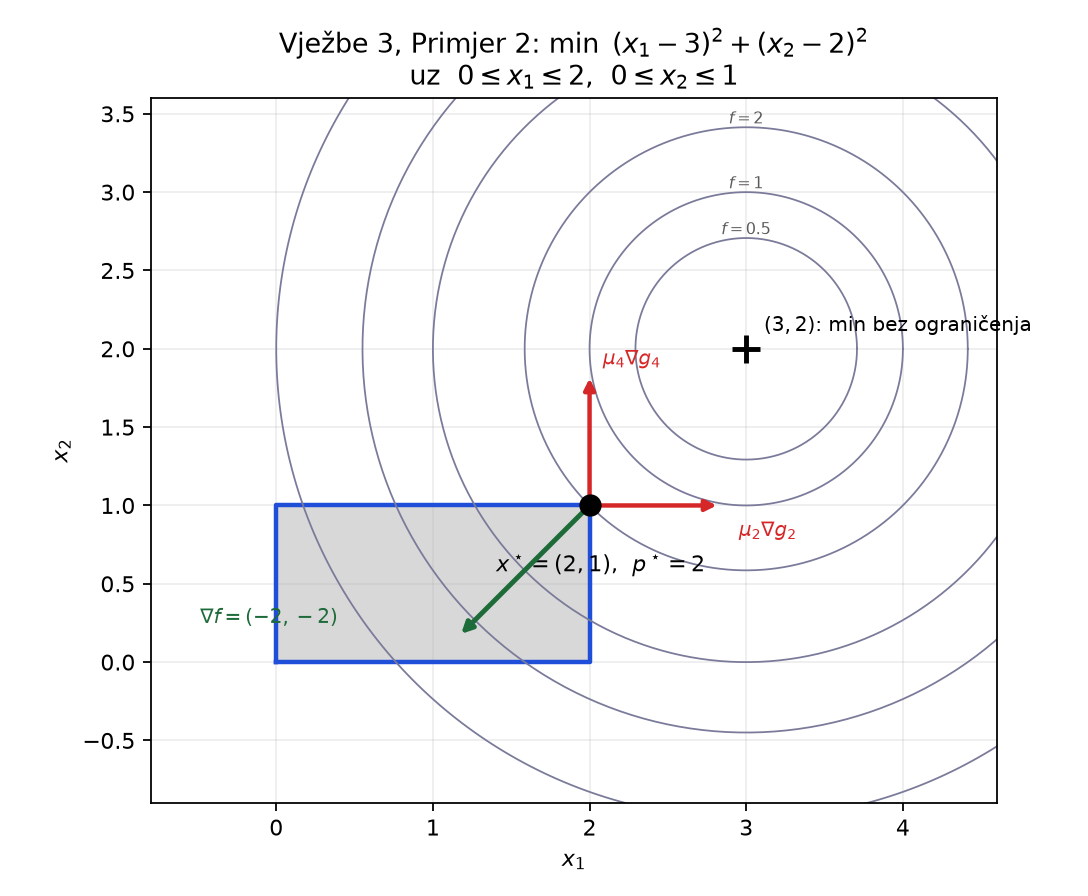
\includegraphics[width=0.80\textwidth]{04-primjer2-kkt.png}
\caption{Vježbe 3, Primjer 2. Dozvoljeni skup je pravokutnik, nivo krivulje su
kružnice oko $(3,2)$, a optimum je vrh $(2,1)$ u kojem su aktivna ograničenja
$g_2$ i $g_4$. Gradijent cilja (zeleno) uravnotežen je zbrojem
$\mu_2\nabla g_2 + \mu_4\nabla g_4$ (crveno).}
\end{figure}

\begin{crtanje}[KKT točka u vrhu pravokutnika]
\textbf{Korak 1.} Nacrtajte osi $x_1$ (od $-1$ do $4{,}5$) i $x_2$ (od $-1$ do
$3{,}5$), jednakim mjerilom.

\textbf{Korak 2 --- prvo ograničenje $g_1$: $-x_1 \le 0$, tj.\ $x_1 \ge 0$.}
Granica je okomita os; dopušteno je \textbf{desno} od nje.

\textbf{Korak 3 --- drugo ograničenje $g_2$: $x_1 \le 2$.} Granica je okomiti
pravac kroz $x_1 = 2$; dopušteno je \textbf{lijevo}. Zajedno s korakom 2 imamo
okomitu traku $0 \le x_1 \le 2$.

\textbf{Korak 4 --- treće i četvrto ograničenje: $0 \le x_2 \le 1$.} Analogno,
vodoravna traka. Presjek dviju traka je \textbf{pravokutnik}
$[0,2]\times[0,1]$ --- osjenčajte ga. To je dozvoljeni skup (politop, usporedi
odjeljak~\ref{sec:poliedar}).

\textbf{Korak 5 --- ciljna točka.} Označite križićem točku $(3,2)$. Ona je
\emph{izvan} pravokutnika --- gore desno.

\textbf{Korak 6 --- nivo krivulje.} $f = (x_1-3)^2+(x_2-2)^2 = c$ su kružnice
oko $(3,2)$ polumjera $\sqrt c$. Nacrtajte ih za $c = 0{,}5;\ 1;\ 2;\ 4$.
Uočite da kružnica $c = 2$ (polumjer $\approx 1{,}41$) prva dodiruje
pravokutnik.

\textbf{Korak 7 --- optimum.} Dodirna točka je vrh $(2,1)$ --- označite je punom
točkom. Provjera: udaljenost od $(3,2)$ do $(2,1)$ je $\sqrt{1+1}=\sqrt2$, pa
je $f = 2$. \checkmark

\textbf{Korak 8 --- gradijent cilja.} Iz $(2,1)$ nacrtajte
$\nabla f = (-2,-2)$: dvije jedinice lijevo, dvije dolje --- dakle
\emph{u} pravokutnik (prema unutra).

\textbf{Korak 9 --- gradijenti aktivnih ograničenja.} Iz iste točke nacrtajte
$\nabla g_2 = (1,0)$ (udesno) i $\nabla g_4 = (0,1)$ (gore). Skalirajte ih s
$\mu_2 = 2$ odn.\ $\mu_4 = 2$, dakle po dvije jedinice.

\textbf{Korak 10 --- provjera KKT-a okom.} Zbroj crvenih strelica je
$(2,0) + (0,2) = (2,2)$, što je točno $-\nabla f$. Uvjet $(\clubsuit)$ kaže
upravo to: $\nabla f + \mu_2\nabla g_2 + \mu_4\nabla g_4 = 0$.

\textbf{Što graf znači.} U vrhu politopa aktivna su dva ograničenja, pa
$-\nabla f$ mora ležati \emph{unutar} kuta razapetog njihovim gradijentima ---
to je stožac iz odjeljka o geometrijskoj interpretaciji \str{3:56}. Da je ciljna
točka bila npr.\ $(3;\ 0{,}5)$, aktivno bi bilo samo $g_2$, i optimum bi bio na
stranici, a ne u vrhu.
\end{crtanje}

% =====================================================================
\section{Numeričko rješavanje i dualni problem}
\label{sec:primjer2-dual}

Ovaj odjeljak nastavlja Zadatak~\ref{zad:primjer2} podzadacima c) i d).

\subsection{c) Rješavanje u MATLAB-u}
\str{V3:28--33}

\textbf{Prevođenje u QP standardnu formu} \str{V3:28}\textbf{.} MATLAB-ova
funkcija \texttt{quadprog} očekuje problem oblika
$\min \tfrac12 x\T Q x + c\T x$ uz $Gx \le h$. Zato ciljnu funkciju treba
raspisati:

\[
\text{minimiziraj}_x \quad
\frac{1}{2}\begin{pmatrix}x_1\\x_2\end{pmatrix}\T
\underbrace{\begin{pmatrix}2&0\\0&2\end{pmatrix}}_{Q}
\begin{pmatrix}x_1\\x_2\end{pmatrix}
+ \underbrace{\begin{pmatrix}-6 & -4\end{pmatrix}}_{c\T}
\begin{pmatrix}x_1\\x_2\end{pmatrix} + 13
\]
\[
\text{uz ogr.}\quad
\underbrace{\begin{pmatrix}
-1 & 0 \\ 1 & 0 \\ 0 & -1 \\ 0 & 1
\end{pmatrix}}_{G}
\begin{pmatrix}x_1\\x_2\end{pmatrix}
\le
\underbrace{\begin{pmatrix}0\\2\\0\\1\end{pmatrix}}_{h}
\]

\emph{Provjera raspisa ciljne funkcije:}
\begin{align}
(x_1-3)^2 + (x_2-2)^2
&= x_1^2 - 6x_1 + 9 + x_2^2 - 4x_2 + 4 \\
&= \underbrace{x_1^2 + x_2^2}_{=\;\frac12(2x_1^2+2x_2^2)\;=\;\frac12 x\T Qx}
 \;\underbrace{-\,6x_1 - 4x_2}_{=\;c\T x}\; + \;13
\end{align}
\checkmark \; Konstanta $13$ ne utječe na $\argmin$, pa je \texttt{quadprog} ne
prima --- ali je treba \textbf{dodati natrag} na dobivenu optimalnu vrijednost.
(To je odgovor na pitanje „zašto $+13$?” s komentara u kodu.)

\textbf{Kod sa slajda} \str{V3:30}:

\begin{verbatim}
Q=[2, 0;  0, 2];
c=[-6; -4];
G=[-1,0;  1,0;  0,-1;  0,1];
h=[0;2;0;1];

[x_opt,f_opt,EXITFLAG,OUTPUT,mu_opt] = quadprog(Q,c,G,h);

x_opt              % optimalne primarne varijable
mu_opt.ineqlin     % optimalne dualne varijable

f_opt+13           % vrijednost funkcije cilja u optimiumu (zasto +13 ?)
\end{verbatim}

\textbf{Ispis rezultata} \str{V3:31}:

\begin{verbatim}
>> x_opt
x_opt =
    2.0000
    1.0000

>> mu_opt.ineqlin
ans =
         0
    2.0000
         0
    2.0000

>> f_opt+13
ans =
    2.0000
\end{verbatim}

\textbf{Poklapanje s ručnim rješenjem:} $x\opt = (2,1)$,
$\mu\opt = (0,2,0,2)$, $p\opt = 2$ --- točno kao u podzadatku b). \checkmark

\textbf{Isti problem preko YALMIP-a} \str{V3:32}\textbf{.} YALMIP je
„modelirajući sloj”: problem se piše prirodnim zapisom, a on ga sam prevede
odabranom rješavaču (ovdje opet \texttt{quadprog}).

\begin{verbatim}
yalmip('clear')
x=sdpvar(2,1);

Con=[0<=x(1)<=2, 0<=x(2)<=1];

Objective=(x(1)-3)^2+(x(2)-2)^2;

% neke opcije YALMIP i "solver"
options = sdpsettings('verbose',1,'solver','quadprog',...
                      'quadprog.maxiter',100);

% Poziv za rjesavanje
sol = optimize(Con,Objective,options);

% Analiza "error zastavica"
if sol.problem == 0
 % Definiraj i ispintaj rjesenje
 x_opt = value(x)     % optimalne primarne
 mu_opt=dual(Con)     % optimalne dualne varijable
else
 display('Nesto je krivo!');
 sol.info
 yalmiperror(sol.problem)
end
\end{verbatim}

\textbf{Ispis} \str{V3:33}\textbf{:} \texttt{x\_opt = [2.0000; 1.0000]},
\texttt{mu\_opt = [0; 2.0000; 0; 2.0000]} --- identično. \checkmark

\begin{napomena}[quadprog vs.\ YALMIP]
\texttt{quadprog} traži da problem \emph{ručno} prevedete u matrice
$Q, c, G, h$ --- što je izvor grešaka, ali daje potpunu kontrolu. YALMIP
prihvaća zapis blizak matematičkom (\texttt{0<=x(1)<=2}) i sam radi prijevod;
zato je pogodniji za veće modele. Obratite pažnju da YALMIP dualne varijable
vraća funkcijom \texttt{dual(Con)}, a \texttt{quadprog} u polju
\texttt{mu\_opt.ineqlin}.
\end{napomena}

\subsection{d) Postavljanje i rješavanje dualnog problema}
\str{V3:34--39}

\textbf{Primarni problem} (u QP formi, bez konstante):
\[
\min_x \; \tfrac12 x\T Qx + c\T x \qquad\text{uz ogr.}\quad Gx - h \le 0
\]

\textbf{Uočimo} (sa slajda): $Q \succ 0$, pa stoga i $Q^{-1}$ postoji ($Q$ nema
svojstvenu vrijednost jednaku nuli jer su sve striktno veće od nule).

\textbf{Korak 1 --- Lagrangian:}
\[
L(x,\mu) = \tfrac12 x\T Qx + c\T x + \mu\T(Gx - h)
         = \tfrac12 x\T Qx + (c\T + \mu\T G)x - \mu\T h
\]

\textbf{Korak 2 --- minimizacija po $x$} \str{V3:35}:
\[
\ell(\mu) = \inf_x L(x,\mu) \;\to\;
\nabla_x L(x,\mu) = 0 \;\to\;
Q\tilde x + c + G\T\mu = 0 \;\to\;
\tilde x = -Q^{-1}(c + G\T\mu)
\]

\emph{Raspis gradijenta:} za kvadratnu formu vrijedi
$\nabla_x(\tfrac12 x\T Qx) = Qx$ (uz simetričan $Q$), a
$\nabla_x\big((c\T+\mu\T G)x\big) = c + G\T\mu$. Član $-\mu\T h$ ne ovisi o
$x$. Izjednačavanjem s nulom i množenjem s $Q^{-1}$ slijeva dobivamo $\tilde x$.
\checkmark

\textbf{Korak 3 --- uvrštavanje natrag} \str{V3:36}:
\begin{align}
\ell(\mu) &= \tfrac12\tilde x\T Q\tilde x + (c\T + \mu\T G)\tilde x - \mu\T h \\
&= -\tfrac12\mu\T GQ^{-1}G\T\mu
   + \big(-c\T Q^{-1}G\T - h\T\big)\mu
   - \tfrac12 c\T Q^{-1}c
\end{align}

\emph{Raspis (na slajdu nije prikazan).} Označimo $z := c + G\T\mu$, pa je
$\tilde x = -Q^{-1}z$ i $(c\T+\mu\T G) = z\T$:
\begin{align}
\tfrac12\tilde x\T Q\tilde x
  &= \tfrac12 z\T Q^{-1}QQ^{-1}z = \tfrac12 z\T Q^{-1}z \\
z\T\tilde x &= -z\T Q^{-1}z \\
\Rightarrow\quad \ell(\mu)
  &= \tfrac12 z\T Q^{-1}z - z\T Q^{-1}z - \mu\T h
   = -\tfrac12 z\T Q^{-1}z - \mu\T h
\end{align}
Sada raspišemo $z\T Q^{-1}z$:
\[
(c + G\T\mu)\T Q^{-1}(c + G\T\mu)
= c\T Q^{-1}c + 2c\T Q^{-1}G\T\mu + \mu\T GQ^{-1}G\T\mu
\]
Uvrštavanjem:
\[
\ell(\mu) = -\tfrac12 c\T Q^{-1}c - c\T Q^{-1}G\T\mu
            - \tfrac12\mu\T GQ^{-1}G\T\mu - h\T\mu
\]
što je točno izraz sa slajda nakon grupiranja linearnih članova. \checkmark

\textbf{Dualni problem} \str{V3:37}:
\[
\max_{\mu \ge 0}\;
-\tfrac12\mu\T GQ^{-1}G\T\mu + \big(-c\T Q^{-1}G\T - h\T\big)\mu
- \tfrac12 c\T Q^{-1}c
\]

\textbf{Tvrdnja sa slajda:} budući da je $-GQ^{-1}G\T \prec 0$, dualni problem
je problem maksimizacije konkavne funkcije s konveksnim ograničenjima
$\to$ \textbf{konveksan optimizacijski problem}.

\begin{napomena}[preciznije o toj tvrdnji]
Općenito vrijedi $-GQ^{-1}G\T \preceq 0$ (negativno \emph{semi}definitno), jer
je $\mu\T GQ^{-1}G\T\mu = (G\T\mu)\T Q^{-1}(G\T\mu) \ge 0$ uz $Q^{-1} \succ 0$
--- ali je nula kad god je $G\T\mu = 0$.

U ovom konkretnom primjeru $G$ ima $4$ retka, a samo $2$ stupca, pa $G\T$ ima
netrivijalnu jezgru i matrica $GQ^{-1}G\T$ \emph{jest} singularna. Konkretno,
uz $Q^{-1} = \tfrac12 I$:
\[
GQ^{-1}G\T = \tfrac12 GG\T = \tfrac12
\begin{pmatrix}
 1 & -1 & 0 & 0 \\
-1 & 1 & 0 & 0 \\
 0 & 0 & 1 & -1 \\
 0 & 0 & -1 & 1
\end{pmatrix}
\]
čije su svojstvene vrijednosti $0, 0, 1, 1$. Dakle striktna negativna
definitnost sa slajda je preoštra; ispravno je $\preceq 0$. \textbf{Zaključak
ostaje isti} --- za konkavnost je dovoljna semidefinitnost, pa je dualni
problem i dalje konveksan.
\end{napomena}

\textbf{Kod za rješavanje dualnog problema} \str{V3:38}:

\begin{verbatim}
Q=[2, 0;  0, 2];
c=[-6; -4];
G=[-1,0;  1,0;  0,-1;  0,1];
h=[0;2;0;1];

Q_dual=G*inv(Q)*G';
c_dual=G*inv(Q)*c+h;
G_dual=-eye(4);
h_dual=zeros(4,1);

[mu_opt_Dual,f_opt_Dual] = quadprog(Q_dual,c_dual,G_dual,h_dual);

mu_opt_Dual   % optimalne dualne varijable

x_opt_Dual=-inv(Q)*(c+G'*mu_opt_Dual)   % optimalne primarne varijable

% vrijednost dualne funkcije cilja u optimiumu:
f_opt_Dual=(-f_opt_Dual+13)-0.5*c'*inv(Q)*c
\end{verbatim}

\textbf{Kako je kod dobiven iz formule} --- vrijedi ga pročitati redak po redak:

\begin{itemize}
  \item \texttt{quadprog} \emph{minimizira}, a mi \emph{maksimiziramo}, pa se
        koristi trik $\max \ell \Leftrightarrow \min(-\ell)$
        (odjeljak~\ref{sec:trikovi}). Zato \texttt{Q\_dual} $= GQ^{-1}G\T$ (bez
        minusa) i \texttt{c\_dual} $= GQ^{-1}c + h$.
  \item Ograničenje $\mu \ge 0$ piše se u obliku $G_{\text{dual}}\mu \le
        h_{\text{dual}}$ uz $G_{\text{dual}} = -I$ i $h_{\text{dual}} = 0$, tj.\
        $-\mu \le 0$.
  \item \texttt{x\_opt\_Dual} rekonstruira primarnu varijablu iz formule
        $\tilde x = -Q^{-1}(c + G\T\mu)$ --- \textbf{primarno rješenje se dobiva
        iz dualnog}, što je moguće upravo zbog jake dualnosti.
  \item Zadnji redak vraća predznak i dodaje konstante: $+13$ (izbačena iz
        cilja) i $-\tfrac12 c\T Q^{-1}c$ (član koji \texttt{quadprog} ne vidi).
\end{itemize}

\textbf{Ispis} \str{V3:39}:

\begin{verbatim}
mu_opt_Dual =        x_opt_Dual =        f_opt_Dual =
    0.0000               2.0000              2.0000
    2.0000               1.0000
    0.0000
    2.0000
\end{verbatim}

\textbf{Provjera jake dualnosti:} $d\opt = 2 = p\opt$. \checkmark Dualne
varijable dobivene rješavanjem \emph{dualnog} problema identične su onima koje
je \texttt{quadprog} vratio kao nusprodukt rješavanja \emph{primarnog} problema.

% =====================================================================
\section{Dualna dekompozicija: distribuirano rješavanje}
\label{sec:dekompozicija}
\str{24--27}

\subsection{Strukturirani problem}
\str{25}

\begin{equation}
\label{eq:strukturiran}
\begin{aligned}
\min_{x_1,x_2} \quad & f_1(x_1) + f_2(x_2) \\
\text{uz ogr.} \quad & x_1 \in \Feas_1, \; x_2 \in \Feas_2 \\
& h_1(x_1) + h_2(x_2) = 0 && (\spadesuit)
\end{aligned}
\end{equation}

\textbf{Opažanje sa slajda:} kad ne bi bilo ograničenja $(\spadesuit)$ koje
„povezuje” $x_1$ i $x_2$, ovaj optimizacijski problem bi se sveo na
\textbf{dva neovisna} optimizacijska problema.

\textbf{Struktura problema.} Funkcija cilja je \emph{separabilna} (zbroj
članova, svaki ovisi o svojoj varijabli), lokalna ograničenja su odvojena, i
samo \emph{jedno} ograničenje $(\spadesuit)$ spaja dva dijela. Takva se
struktura pojavljuje svugdje gdje više jedinica dijeli zajednički resurs.

\subsection{Dualni problem}
\str{26}

\begin{align}
\max_\lambda\; \ell(\lambda)
&= \inf_{x_1\in\Feas_1,\,x_2\in\Feas_2}
   f_1(x_1) + f_2(x_2) + \lambda\T\big(h_1(x_1) + h_2(x_2)\big) \\
&= \inf_{x_1\in\Feas_1}\Big(f_1(x_1) + \lambda\T h_1(x_1)\Big)
 + \inf_{x_2\in\Feas_2}\Big(f_2(x_2) + \lambda\T h_2(x_2)\Big)
\end{align}

\emph{Zašto se infimum smije rastaviti:} nakon uvrštavanja $\lambda$ izraz se
raspada na dva dijela, od kojih prvi ovisi \emph{samo} o $x_1$, a drugi
\emph{samo} o $x_2$; varijable više nisu spojene nikakvim zajedničkim
ograničenjem. Minimum zbroja neovisnih članova je zbroj minimuma.

\textbf{Ključno opažanje sa slajda:} \emph{Uočite da smo dualizirali samo
globalno ograničenje $(\spadesuit)$ dok su lokalna ograničenja
$x_1 \in \Feas_1$, $x_2 \in \Feas_2$ ostavljena u definiciji od $\ell(\lambda)$.}

\begin{napomena}[djelomična dualizacija]
Nije nužno dualizirati \emph{sva} ograničenja. Bira se ono čije uklanjanje
razbija strukturu problema --- ovdje globalno ograničenje. Lokalna ostaju kao
ograničenja unutarnjih podproblema. To je bit tehnike.
\end{napomena}

\subsection{Algoritam}
\str{27}

Za zadani fiksni $\lambda$ imamo \textbf{dva neovisna podproblema} (mogu se
rješavati odvojeno / paralelno):

\begin{itemize}
  \item \textbf{podproblem 1:}
        $\inf_{x_1\in\Feas_1}\big(f_1(x_1) + \lambda\T h_1(x_1)\big)$,
        koji ima opt.\ vrijednost $\ell_1(\lambda)$;
  \item \textbf{podproblem 2:}
        $\inf_{x_2\in\Feas_2}\big(f_2(x_2) + \lambda\T h_2(x_2)\big)$,
        koji ima opt.\ vrijednost $\ell_2(\lambda)$.
\end{itemize}

\textbf{Dualni problem} (koji rješava i primarni, uz jaku dualnost):
\[
\max_\lambda\; \ell(\lambda) = \ell_1(\lambda) + \ell_2(\lambda)
\]

\textbf{Rješenje dualnog problema se postiže kad je $h_1(x_1) + h_2(x_2) = 0$.}

\begin{napomena}[kako to izgleda kao algoritam]
Postupak je iterativan i ima strukturu „koordinator + jedinice”:
\begin{enumerate}
  \item koordinator objavi trenutni $\lambda$;
  \item svaka jedinica \emph{neovisno} riješi svoj mali problem i javi svoj
        $h_i(x_i)$;
  \item koordinator pogleda „neravnotežu” $h_1 + h_2$ i prilagodi $\lambda$
        (poveća ga ako je zbroj pozitivan, smanji ako je negativan);
  \item ponovi dok neravnoteža ne padne na nulu.
\end{enumerate}
Uočite koliko se malo informacija razmjenjuje: jedinice \textbf{ne moraju
otkriti} svoje funkcije $f_i$, $h_i$ ni svoje skupove $\Feas_i$ --- samo jedan
broj. To je ključno u primjeni koja slijedi.
\end{napomena}

% =====================================================================
\section{Vježbe 3, Primjer 1: tržište i formiranje cijena}
\label{sec:trziste}
\str{V3:3--18}

Ovo je izravna primjena dualne dekompozicije --- i objašnjenje najave iz
poglavlja~\ref{ch:uvod} \str{1:34}: \emph{matematička formulacija tržišta i
kreiranja tržišnih cijena je Lagrangeova dualnost}.

\subsection{Postavka: maksimizacija društvene dobrobiti}
\str{V3:4}

\textbf{Oznake:}
\begin{itemize}
  \item Troškovi proizvodnje za $i$-tog proizvođača za proizvodnju $p_i$ [MWh]
        energije: $C_i(p_i)$.
  \item Funkcija benefita za $j$-tog potrošača kod potrošnje $d_j$ [MWh]
        energije: $B_j(d_j)$.
\end{itemize}

\textbf{Maksimizacija društvene dobrobiti:}
\begin{equation}
\label{eq:trziste}
\begin{aligned}
\min_{p_1,\dots,p_n,\,d_1,\dots,d_m} \quad
& \sum_{i=1}^{n}C_i(p_i) - \sum_{j=1}^{m}B_j(d_j)
  && (=\ \max\ \text{društvena dobrobit}) \\
\text{uz ogr.} \quad
& p_i \in P_i, \; i = 1,\dots,n
  && \text{(lokalna ograničenja proizvođača)} \\
& d_j \in D_j, \; j = 1,\dots,m
  && \text{(lokalna ograničenja potrošača)} \\
& \sum_{i=1}^{n}p_i = \sum_{j=1}^{m}d_j
  && \text{(balans potrošnje i proizvodnje)}
\end{aligned}
\end{equation}

\textbf{Primjeri lokalnih ograničenja} (sa slajda):
\[
P_i := \{\, p \mid \underline{p_i} \le p \le \overline{p_i} \,\}, \qquad
D_j := \{\, d \mid \underline{d_j} \le d \le \overline{d_j} \,\}
\]
--- dakle svaka elektrana ima minimalnu i maksimalnu snagu, svaki potrošač
minimalnu i maksimalnu potrošnju.

\textbf{Kako čitati funkciju cilja.} \emph{Društvena dobrobit} je ukupna korist
potrošača umanjena za ukupni trošak proizvodnje,
$\sum_j B_j(d_j) - \sum_i C_i(p_i)$. Nju želimo \emph{maksimizirati}, pa
minimiziramo njezinu negaciju --- odatle poredak članova u
\eqref{eq:trziste} (trik $\max f \Leftrightarrow \min(-f)$,
odjeljak~\ref{sec:trikovi}).

\textbf{Pretpostavka konveksnosti} \str{V3:6}\textbf{:} $C_i(\cdot)$ konveksne
funkcije, $B_j(\cdot)$ \textbf{konkavne} funkcije, $P_i$, $D_j$ konveksni
skupovi.

\begin{napomena}[zašto baš takve pretpostavke]
\begin{itemize}
  \item $C_i$ konveksna: trošak proizvodnje raste \emph{sve brže} --- svaki
        sljedeći MWh je skuplji (uključuju se sve skuplji agregati). To je
        realistično.
  \item $B_j$ konkavna: korist raste \emph{sve sporije} --- zakon opadajuće
        granične korisnosti. Prvi MWh vrijedi mnogo, deseti mnogo manje.
  \item Uz to je $-B_j$ konveksna, pa je \textbf{cijela funkcija cilja
        konveksna} --- problem \eqref{eq:trziste} je konveksan i vrijedi jaka
        dualnost.
\end{itemize}
\end{napomena}

\subsection{Dualni problem}
\str{V3:5--9}

\textbf{Primarni problem} \str{V3:5}:
\[
\min_{p_i\in P_i,\,d_j\in D_j}\;
\sum_{i=1}^{n}C_i(p_i) - \sum_{j=1}^{m}B_j(d_j)
\qquad\text{uz ogr.}\quad \sum_{i=1}^{n}p_i = \sum_{j=1}^{m}d_j
\]

\textbf{Dualni problem} \str{V3:6}:
\[
\max_{\lambda\in\R}\; \ell(\lambda), \quad\text{gdje je}\quad
\ell(\lambda) = \min_{p_i\in P_i,\,d_j\in D_j}
\sum_{i=1}^{n}C_i(p_i) - \sum_{j=1}^{m}B_j(d_j)
+ \lambda\left(\sum_{j=1}^{m}d_j - \sum_{i=1}^{n}p_i\right)
\]

\textbf{Napomena sa slajda} \str{V3:7}\textbf{:} \emph{Uočite da smo dualizirali
samo globalno ograničenje $\sum_j d_j - \sum_i p_i = 0$ dok su ostala lokalna
ograničenja ostavljena u definiciji od $\ell(\lambda)$.}

\textbf{Opažanje 1} \str{V3:8}\textbf{:} Lagrangeova dualna funkcija
$\ell(\lambda)$ se za fiksan $\lambda$ može rastaviti u \textbf{$n + m$
odvojenih minimizacijskih problema}.

\textbf{Opažanje 2} \str{V3:9}\textbf{:} $\max_{\lambda\in\R}\ell(\lambda)$ se
postiže kad je $\sum_{j=1}^{m}d_j = \sum_{i=1}^{n}p_i$ ((sub)gradijent od
$\ell(\lambda)$ je nula).

\subsection{Rastav na lokalne probleme}
\str{V3:10}

\begin{center}
\begin{tabular}{P{6.4cm}P{6.4cm}}
\toprule
\textbf{Lokalna minimizacija proizvođača} &
\textbf{Lokalna minimizacija potrošača} \\
$\to$ maksimizacija svoje zarade &
$\to$ maksimizacija svog benefita \\
\midrule
$\displaystyle\min_{p_1\in P_1} C_1(p_1) - \lambda p_1$ &
$\displaystyle\min_{d_1\in D_1} \lambda d_1 - B_1(d_1)$ \\[6pt]
$\displaystyle\min_{p_2\in P_2} C_2(p_2) - \lambda p_2$ &
$\displaystyle\min_{d_2\in D_2} \lambda d_2 - B_2(d_2)$ \\[2pt]
\quad$\vdots$ & \quad$\vdots$ \\[2pt]
$\displaystyle\min_{p_n\in P_n} C_n(p_n) - \lambda p_n$ &
$\displaystyle\min_{d_m\in D_m} \lambda d_m - B_m(d_m)$ \\
\bottomrule
\end{tabular}
\end{center}

\textbf{Interpretacija --- ovo je srce cijelog primjera:}

\begin{itemize}
  \item $C_i(p_i) - \lambda p_i$ je \textbf{negativna zarada} proizvođača:
        $\lambda p_i$ je prihod od prodaje $p_i$ MWh po cijeni $\lambda$, a
        $C_i(p_i)$ je trošak. Minimizacija tog izraza = maksimizacija profita.
  \item $\lambda d_j - B_j(d_j)$ je \textbf{negativna korist} potrošača:
        $\lambda d_j$ je ono što plaća, $B_j(d_j)$ je korist koju ima.
  \item Dakle: \textbf{svaki sudionik gleda samo svoj interes}, koristeći samo
        \emph{svoju} funkciju i \emph{jedan zajednički broj} $\lambda$.
\end{itemize}

\begin{napomena}[tipfeler na slajdovima V3:10--11]
U stupcu potrošača na slajdu svugdje piše $B_1(\cdot)$, i za drugog i za
$m$-tog potrošača. Ispravno je $B_2(d_2)$, \dots, $B_m(d_m)$ --- svaki potrošač
ima svoju funkciju benefita.
\end{napomena}

\subsection{Uloga operatora tržišta}
\str{V3:11}

\begin{center}
\begin{tabular}{P{13.0cm}}
\toprule
\textbf{Operator tržišta:} \quad
$\displaystyle\max_{\lambda\in\R}\ell(\lambda)
\quad\Longleftrightarrow\quad
\text{odredi }\lambda:\; \sum_{j=1}^{m}d_j\opt = \sum_{i=1}^{n}p_i\opt$ \\
\bottomrule
\end{tabular}
\end{center}

\textbf{Racionalno ponašanje sudionika} (max svoj benefit):
\[
p_i\opt = \argmin_{p_i\in P_i} C_i(p_i) - \lambda p_i, \qquad
d_j\opt = \argmin_{d_j\in D_j} \lambda d_j - B_j(d_j)
\]

\begin{teorem}[Glavni rezultat \str{V3:11}]
$\lambda\opt$ koji rješava ovaj problem $=$ \textbf{tržišna cijena energije}.
\end{teorem}

\textbf{Zašto je to fascinantno.} Dualna varijabla, uvedena kao čisto
matematička pomoć, ispada \textbf{cijena}. Nitko ne mora znati tuđe troškove ni
funkcije koristi; svatko optimira svoj interes uz objavljenu cijenu, a operator
samo podešava cijenu dok se ponuda i potražnja ne izjednače. Rezultat je
\textbf{globalno optimalna} raspodjela --- jer je to rješenje dualnog problema,
a uz jaku dualnost i primarnog.

Ovo je ujedno i matematički sadržaj metafore o „nevidljivoj ruci tržišta”.

\subsection{Marginalni troškovi i tržišna cijena}
\str{V3:12}

\textbf{Tvrdnja.} Neka je $\lambda$ takav da je $p_i\opt \in$ unutrašnjost od
$P_i$, $d_j\opt \in$ unutrašnjost od $D_j$; tada imamo
\[
\frac{\dd C_i(p_i\opt)}{\dd p_i} = \lambda, \qquad
\frac{\dd B_j(d_j\opt)}{\dd d_j} = \lambda
\]

\emph{Odakle:} ako je optimum u \emph{unutrašnjosti} lokalnog skupa, lokalna
ograničenja su neaktivna, pa vrijedi obični uvjet stacionarnosti
(odjeljak~\ref{sec:uvjeti-bez-ogr}): derivacija cilja po varijabli je nula.
Za proizvođača: $\dfrac{\dd}{\dd p_i}\big(C_i(p_i) - \lambda p_i\big)
= C_i'(p_i) - \lambda = 0$. \checkmark Analogno za potrošača:
$\lambda - B_j'(d_j) = 0$.

\textbf{Zaključak sa slajda:} \emph{društvena dobrobit je maksimizirana kad svi
potrošači i proizvođači postave nivo proizvodnje/potrošnje tako da su
inkrementalni (marginalni) troškovi/benefiti jednaki tržišnoj cijeni $\lambda$.}

\begin{napomena}[marginalni trošak]
\textbf{Marginalni (inkrementalni) trošak} $\dd C/\dd p$ je trošak proizvodnje
\emph{jednog dodatnog} MWh. Uvjet kaže: proizvodi sve dok te sljedeći MWh košta
manje nego što za njega dobivaš; stani kad se izjednače. Isto vrijedi za
potrošača s koristi. \textbf{U optimumu su svi marginalni troškovi i sve
marginalne koristi jednaki --- i to baš cijeni $\lambda$.}
\end{napomena}

\subsection{Krivulje ponude i potražnje}
\str{V3:13--14}

Iz uvjeta marginalnosti dobivaju se \textbf{krivulje ponude i potražnje}:
\[
\frac{\dd C_i(p_i)}{\dd p_i} = \lambda
\;\Leftrightarrow\; p_i = \gamma_i^p(\lambda)
\;\Leftrightarrow\; \lambda = \beta_i^p(p_i)
\]
\[
\frac{\dd B_j(d_j)}{\dd d_j} = \lambda
\;\Leftrightarrow\; d_j = \gamma_j^d(\lambda)
\;\Leftrightarrow\; \lambda = \beta_j^d(d_j)
\]

To je ista relacija napisana na tri načina: kao jednadžba, kao „koliko
proizvodim pri cijeni $\lambda$” ($\gamma$), i kao „pri kojoj cijeni proizvodim
$p_i$” ($\beta$) --- dakle inverzne funkcije jedna drugoj.

\textbf{Određivanje tržišne cijene u praksi} \str{V3:14}\textbf{.} Cijena
$\lambda\opt$ nalazi se na sjecištu \textbf{agregirane krivulje ponude}
$\tilde\gamma^p(\lambda) := \sum_i\gamma_i^p(\lambda)$ s \textbf{agregiranom
krivuljom potražnje} $\tilde\gamma^d(\lambda) := \sum_j\gamma_j^d(\lambda)$:
\[
\sum_{i=1}^{n}p_i\opt = \sum_{i=1}^{n}\gamma_i^p(\lambda\opt)
= \tilde\gamma^p(\lambda\opt) = \tilde\gamma^d(\lambda\opt)
= \sum_{j=1}^{m}\gamma_j^d(\lambda\opt) = \sum_{j=1}^{m}d_j\opt
\]

\textbf{Napomena sa slajda:} generalizacija na slučajeve kad ne vrijedi da je
$p_i\opt \in$ unutrašnjost od $P_i$, $d_j\opt \in$ unutrašnjost od $D_j$ je
moguća. Lokalna ograničenja mogu se uključiti u krivulje ponude/potražnje.

\textbf{Slika sa slajda} \str{V3:15}\textbf{.} Prikazana su tri grafa:

\begin{itemize}
  \item gore lijevo „\emph{Supply}”: os $\lambda$ okomito, os $p$ vodoravno;
        nekoliko stepenastih rastućih krivulja (po jedna za svakog
        proizvođača);
  \item gore desno „\emph{Demand}”: os $\lambda$ okomito, os $d$ vodoravno;
        nekoliko stepenastih \emph{padajućih} krivulja;
  \item dolje: dvije strelice vode prema trećem grafu, na kojem su
        \textbf{agregirane} krivulje --- rastuća (ponuda) i padajuća
        (potražnja). Njihovo sjecište označeno je crvenom točkom; na osi
        $\lambda$ očitava se $\lambda^{*}$, a na vodoravnoj osi („\emph{power}”)
        očitava se $\sum p_i^{*} = \sum d_j^{*}$.
\end{itemize}

\begin{crtanje}[određivanje tržišne cijene]
\textbf{Korak 1.} Nacrtajte koordinatni sustav: vodoravno \emph{količina
energije} (snaga), okomito \emph{cijena} $\lambda$.

\textbf{Korak 2 --- krivulja ponude.} Poredajte proizvođače po marginalnom
trošku, od najjeftinijeg prema najskupljem. Crtajte stepenice slijeva nadesno:
širina stepenice je kapacitet tog proizvođača, visina njegov marginalni trošak.
Dobivate \textbf{rastuću} stepenastu krivulju --- to je agregirana ponuda
$\tilde\gamma^p$.

\emph{Zašto raste:} prvo se uključuju najjeftiniji izvori; što više energije
treba, to skuplje agregate moramo pokrenuti.

\textbf{Korak 3 --- krivulja potražnje.} Isto, ali za potrošače poredane po
marginalnoj koristi, od najviše prema najnižoj. Dobivate \textbf{padajuću}
stepenastu krivulju $\tilde\gamma^d$.

\emph{Zašto pada:} najprije se zadovoljavaju potrebe koje potrošač najviše
cijeni; dodatna potrošnja vrijedi mu sve manje.

\textbf{Korak 4 --- sjecište.} Dvije se krivulje sijeku u jednoj točki.
Označite je. Iz nje povucite vodoravnu isprekidanu crtu do osi $\lambda$ ---
tamo očitajte \textbf{tržišnu cijenu} $\lambda^{*}$. Povucite i okomitu
isprekidanu crtu do vodoravne osi --- tamo očitajte \textbf{količinu}
$\sum p_i^{*} = \sum d_j^{*}$.

\textbf{Korak 5 --- što graf znači.} Lijevo od sjecišta ponuda je jeftinija od
onoga što potrošači vrednuju --- svaka takva transakcija povećava društvenu
dobrobit i \emph{treba} se dogoditi. Desno od sjecišta proizvodnja bi koštala
više nego što vrijedi --- takve transakcije smanjuju dobrobit. Sjecište je
točka gdje se to izjednači, dakle upravo optimum problema
\eqref{eq:trziste}, a $\lambda^{*}$ je dualna varijabla balansnog ograničenja.
\end{crtanje}

\begin{figure}[H]
\centering
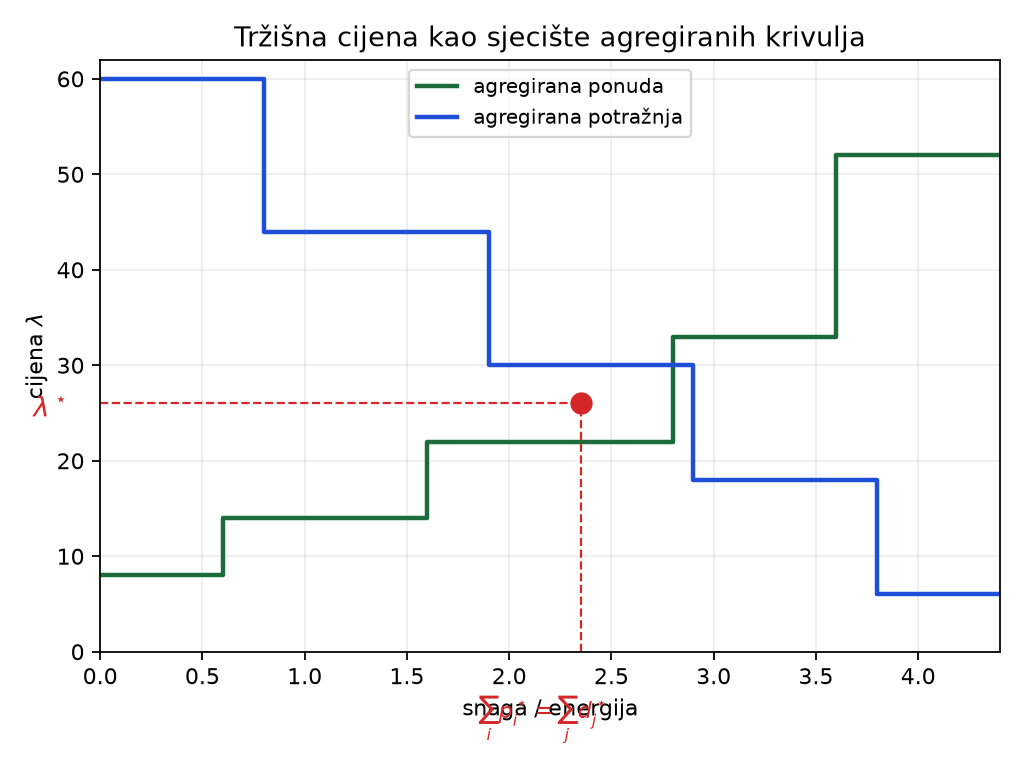
\includegraphics[width=0.74\textwidth]{04-ponuda-potraznja.png}
\caption{Tržišna cijena $\lambda^\star$ kao sjecište agregirane krivulje ponude
(rastuća) i potražnje (padajuća). Rekonstrukcija sheme s Vježbi 3, str.\ 15.}
\end{figure}

\textbf{Stvarni podaci sa slajdova} \str{V3:17--18}\textbf{.} Slajdovi
prikazuju agregirane krivulje burze \textbf{APX} (Amsterdam Power Exchange) za
dva termina istog dana:

\begin{itemize}
  \item \textbf{30.\ siječnja 2015., 2 h ujutro} --- noćni sat, niska
        potražnja: krivulja potražnje je pomaknuta ulijevo, pa je sjecište
        \emph{niže} na osi cijena;
  \item \textbf{30.\ siječnja 2015., 19 h} --- večernji vršni sat, visoka
        potražnja: krivulja potražnje je pomaknuta udesno, sjecište je na
        \emph{strmom} dijelu krivulje ponude, pa je cijena znatno viša.
\end{itemize}

\textbf{Poruka:} teorija s prethodnih slajdova doslovno je mehanizam po kojem
europske burze električne energije svakodnevno formiraju cijenu.

% =====================================================================
\section{Analiza osjetljivosti}
\label{sec:osjetljivost}
\str{28--34}

Zadnja tema poglavlja odgovara na pitanje: \emph{koliko se optimum promijeni ako
malo pomaknemo ograničenja?}

\subsection{Perturbiran problem}
\str{29--31}

\textbf{Polazni par problema} \str{29}:

\begin{center}
\begin{tabular}{P{6.3cm}P{7.0cm}}
\toprule
\textbf{Primarni problem} & \textbf{Dualni problem} \\
\midrule
$\displaystyle\min_x f(x)$ &
$\displaystyle\max_{\lambda,\mu}\;
\ell(\lambda,\mu) := \inf_x\big(f(x) + \lambda\T h(x) + \mu\T g(x)\big)$ \\
uz ogr.\ $h_i(x) = 0$, $i=1,\dots,m$ & uz ogr.\ $\mu \ge 0$ \\
\phantom{uz ogr.\ }$g_j(x) \le 0$, $j=1,\dots,p$ & \\
\bottomrule
\end{tabular}
\end{center}

\textbf{Perturbiran optimizacijski problem} \str{30}:

\begin{center}
\begin{tabular}{P{6.3cm}P{7.0cm}}
\toprule
\textbf{Primarni problem} & \textbf{Dualni problem} \\
\midrule
$\displaystyle\min_x f(x)$ &
$\displaystyle\max_{\lambda,\mu}\;
\ell(\lambda,\mu) - \lambda\T u - \mu\T v$ \\
uz ogr.\ $h_i(x) = u_i$, $i=1,\dots,m$ & uz ogr.\ $\mu \ge 0$ \\
\phantom{uz ogr.\ }$g_j(x) \le v_j$, $j=1,\dots,p$ & \\
\bottomrule
\end{tabular}
\end{center}

gdje su $u = [u_1 \dots u_m]\T$, $v = [v_1 \dots v_p]\T$
\textbf{perturbacijski parametri}.

\emph{Odakle dualni oblik:} Lagrangian perturbiranog problema je
$f(x) + \lambda\T(h(x) - u) + \mu\T(g(x) - v)
= L(x,\lambda,\mu) - \lambda\T u - \mu\T v$. Zadnja dva člana ne ovise o $x$, pa
prolaze kroz $\inf_x$ i ostaju u dualnoj funkciji. \checkmark

\textbf{Značenje parametara.}
\begin{itemize}
  \item $v_j > 0$ znači \textbf{relaksaciju} $j$-tog ograničenja (dopuštamo
        više), $v_j < 0$ znači \textbf{pooštravanje};
  \item $u_i$ pomiče ciljanu vrijednost jednakosti.
\end{itemize}

Neka je $p\opt(u,v)$ opt.\ vrijednost primarnog problema, kao funkcija od $u$ i
$v$; $p\opt(0,0)$ je optimalna vrijednost \textbf{neperturbiranog} primarnog
problema.

\subsection{Globalna osjetljivost}
\str{32--33}

\textbf{Pretpostavimo jaku dualnost} za neperturbiran problem i neka su
$\lambda\opt, \mu\opt$ optimalne dualne varijable primarnog problema (stoga je
nužno $\mu\opt \ge 0$).

\textbf{Izvod (sa slajda 32, korak po korak):}

\begin{enumerate}
  \item Ako primijenimo \emph{slabu} dualnost na \emph{perturbiran} problem,
        imamo
        \[
        p\opt(u,v) \ge \ell(\lambda\opt,\mu\opt)
                     - (\lambda\opt)\T u - (\mu\opt)\T v
        \]
        jer je desna strana Lagrangeova dualna funkcija za perturbiran problem
        (vidjeti prethodni slajd), izračunata u jednom konkretnom dopuštenom
        paru $(\lambda\opt,\mu\opt)$ --- a svaka takva vrijednost je donja
        granica.
  \item Zbog \emph{jake} dualnosti za neperturbiran problem i iz definicije
        $\lambda\opt,\mu\opt$ imamo da je
        $\ell(\lambda\opt,\mu\opt) = p\opt(0,0)$, pa gornja nejednakost implicira
\end{enumerate}

\begin{teorem}[Globalna nejednakost osjetljivosti \str{33}]
\begin{equation}
\label{eq:globalna-osjetljivost}
p\opt(u,v) \ge p\opt(0,0) - (\lambda\opt)\T u - (\mu\opt)\T v
\end{equation}
\end{teorem}

\textbf{Implikacije (sve doslovno sa slajda 33):}

\begin{itemize}
  \item ako je $\mu_j\opt$ \textbf{velik}: $p\opt$ \textbf{znatno raste} ako
        „stisnemo” ograničenje $g_j(x)\le0$ na $g_j(x)\le v_j$ gdje je
        $v_j < 0$;
  \item ako je $\mu_j\opt$ \textbf{malen}: $p\opt$ \textbf{se ne smanjuje
        znatno} ako „relaksiramo” ograničenje $g_j(x)\le0$ na $g_j(x)\le v_j$
        gdje je $v_j > 0$;
  \item ako je $\lambda_i\opt$ \textbf{velik i pozitivan}: $p\opt$ raste znatno
        ako umjesto $h_i(x)=0$ imamo $h_i(x)=u_i$ gdje je $u_i < 0$;
  \item ako je $\lambda_i\opt$ \textbf{velik i negativan}: $p\opt$ raste znatno
        ako umjesto $h_i(x)=0$ imamo $h_i(x)=u_i$ gdje je $u_i > 0$;
  \item ako je $\lambda_i\opt$ \textbf{malen i pozitivan}: $p\opt$ se ne
        smanjuje znatno ako umjesto $h_i(x)=0$ imamo $h_i(x)=u_i$ gdje je
        $u_i > 0$;
  \item ako je $\lambda_i\opt$ \textbf{malen i negativan}: $p\opt$ se ne
        smanjuje znatno ako umjesto $h_i(x)=0$ imamo $h_i(x)=u_i$ gdje je
        $u_i < 0$.
\end{itemize}

\begin{napomena}[kako zapamtiti smjer]
Pogledajte \eqref{eq:globalna-osjetljivost}: član $-(\mu\opt)\T v$ ulazi s
\emph{minusom}. Dakle relaksacija ($v_j > 0$) \textbf{spušta} donju granicu za
$p\opt$ --- optimum se smije poboljšati (smanjiti), i to najviše za
$\mu_j\opt v_j$. Pooštravanje ($v_j < 0$) \textbf{diže} granicu --- optimum se
\emph{nužno} pogorša barem za $|\mu_j\opt v_j|$.

Uočite asimetriju: kod pooštravanja \eqref{eq:globalna-osjetljivost} daje
\textbf{jamstvo} (donja granica je čvrsta), a kod relaksacije samo
\emph{gornju ocjenu} mogućeg poboljšanja. Zato je gornja tablica formulirana s
„raste znatno” u jednom, a „ne smanjuje se znatno” u drugom smjeru.
\end{napomena}

\subsection{Lokalna osjetljivost}
\str{34}

\begin{teorem}[Lokalna osjetljivost]
Pretpostavimo jaku dualnost za neperturbiran problem i neka su
$\lambda\opt, \mu\opt$ optimalne dualne varijable primarnog problema.

Ako je $p\opt(u,v)$ diferencijabilno u $(0,0)$, tada vrijedi
\begin{equation}
\label{eq:lokalna-osjetljivost}
\lambda_i\opt = -\frac{\partial p\opt(0,0)}{\partial u_i}, \qquad
\mu_i\opt = -\frac{\partial p\opt(0,0)}{\partial v_i}
\end{equation}
\end{teorem}

\textbf{Ovo je najkorisnija formula poglavlja.} Ona kaže da Lagrangeov
množitelj \emph{jest} derivacija optimalne vrijednosti po pomaku ograničenja
--- dakle broj s izravnim inženjerskim i ekonomskim značenjem:

\begin{itemize}
  \item $\mu_j\opt$ mjeri \textbf{koliko bi se $p\opt$ popravio} kad bismo
        $j$-to ograničenje popustili za jednu jedinicu;
  \item ograničenja s $\mu_j\opt = 0$ su \textbf{neaktivna} --- njihovo
        popuštanje ne donosi ništa (usporedi uvjet komplementarnosti);
  \item u ekonomiji se $\mu_j\opt$ zove \textbf{sjenska cijena} (engl.\
        \emph{shadow price}) resursa: najviše što bismo bili spremni platiti za
        dodatnu jedinicu tog resursa.
\end{itemize}

Time se zatvara krug s fizikalnom interpretacijom iz
poglavlja~\ref{ch:uvjeti} \str{3:62--63}: množitelj je \emph{reakcija veze} ---
mjera koliko ograničenje „gura”.

\subsection{Vježbe 3, Primjer 2, podzadaci e) i f)}

\begin{zadatak}[Nastavak Zadatka~\ref{zad:primjer2}: osjetljivost]
\str{V3:40--42}

\textbf{e) Što možete reći o osjetljivosti optimalne vrijednosti na
perturbacije u ograničenjima?}

\textbf{Perturbirani problem} \str{V3:40}:
\[
\text{minimiziraj}_x \quad
\frac{1}{2}\begin{pmatrix}x_1\\x_2\end{pmatrix}\T
\underbrace{\begin{pmatrix}2&0\\0&2\end{pmatrix}}_{Q}
\begin{pmatrix}x_1\\x_2\end{pmatrix}
+ \underbrace{\begin{pmatrix}-6&-4\end{pmatrix}}_{c\T}
\begin{pmatrix}x_1\\x_2\end{pmatrix} + 13
\]
\[
\text{uz ogr.}\quad
\underbrace{\begin{pmatrix}
-1 & 0 \\ 1 & 0 \\ 0 & -1 \\ 0 & 1
\end{pmatrix}}_{G}
\begin{pmatrix}x_1\\x_2\end{pmatrix}
- \underbrace{\begin{pmatrix}0\\2\\0\\1\end{pmatrix}}_{h}
\le \begin{pmatrix}v_1\\v_2\\v_3\\v_4\end{pmatrix}
\]
Optimalno rješenje: $p\opt(v_1,v_2,v_3,v_4)$.

\textbf{Rješenje} \str{V3:41}\textbf{.} Budući da je
$\mu\opt = \begin{pmatrix}0 & 2 & 0 & 2\end{pmatrix}\T$, imamo (primjenom
\eqref{eq:lokalna-osjetljivost}):
\[
\frac{\partial p\opt(0,0,0,0)}{\partial v_1} = 0, \qquad
\frac{\partial p\opt(0,0,0,0)}{\partial v_2} = -2,
\]
\[
\frac{\partial p\opt(0,0,0,0)}{\partial v_3} = 0, \qquad
\frac{\partial p\opt(0,0,0,0)}{\partial v_4} = -2
\]

\textbf{Čitanje rezultata:}

\begin{itemize}
  \item $v_1$ i $v_3$ pripadaju \emph{neaktivnim} ograničenjima
        ($x_1 \ge 0$, $x_2 \ge 0$); njihove derivacije su \textbf{nula} ---
        pomicanje tih granica ne mijenja ništa. Logično: optimum $(2,1)$ je
        daleko od njih.
  \item $v_2$ i $v_4$ pripadaju \emph{aktivnim} ograničenjima ($x_1 \le 2$,
        $x_2 \le 1$); derivacije su $-2$. Popuštanje bilo kojeg od njih za
        malu vrijednost $\varepsilon$ smanjuje $p\opt$ za približno
        $2\varepsilon$.
\end{itemize}

\emph{Brza provjera zdravim razumom.} Ako gornju granicu na $x_1$ pomaknemo s
$2$ na $2 + \varepsilon$, novi optimum je $(2+\varepsilon,\ 1)$, pa
\[
p\opt(\varepsilon) = (2+\varepsilon-3)^2 + (1-2)^2
= (\varepsilon - 1)^2 + 1 = 2 - 2\varepsilon + \varepsilon^2
\]
Derivacija u $\varepsilon = 0$ je $-2$. \checkmark Poklapa se s
$\mu_2\opt = 2$ i formulom $\partial p\opt/\partial v_2 = -\mu_2\opt$.

\medskip
\textbf{f) Ponovite (d) i (e) s promijenjenim ograničenjima} $g_2$ i $g_4$
($g_1$ i $g_3$ ostaju ista): $g_2(x) = x_1 - 1{,}5 \le 0$,
$g_4(x) = x_2 - 1{,}5 \le 0$. \str{V3:42}

\textbf{Rezultat sa slajda:} imamo da je
$\mu\opt = \begin{pmatrix}0 & 3 & 0 & 1\end{pmatrix}\T$, pa je stoga
\[
\frac{\partial p\opt(0,0,0,0)}{\partial v_1} = 0, \qquad
\frac{\partial p\opt(0,0,0,0)}{\partial v_2} = -3,
\]
\[
\frac{\partial p\opt(0,0,0,0)}{\partial v_3} = 0, \qquad
\frac{\partial p\opt(0,0,0,0)}{\partial v_4} = -1
\]

\textbf{Provjera rezultata KKT-om} (slajd daje samo brojke; izvod niže slijedi
postupak iz podzadatka b):

\emph{Korak 1 --- novi dozvoljeni skup.} Sada je
$0 \le x_1 \le 1{,}5$, $0 \le x_2 \le 1{,}5$ --- kvadrat stranice $1{,}5$.
Ciljna točka $(3,2)$ je i dalje gore desno izvan njega, pa je najbliža točka
opet gornji desni vrh: $x\opt = (1{,}5;\ 1{,}5)$.

\emph{Korak 2 --- gradijent cilja u optimumu:}
\[
\nabla f(x\opt) = \begin{pmatrix}2\cdot1{,}5 - 6\\ 2\cdot1{,}5 - 4\end{pmatrix}
= \begin{pmatrix}-3\\-1\end{pmatrix}
\]

\emph{Korak 3 --- KKT jednadžba} (aktivni su $g_2$ i $g_4$, pa je
$\mu_1 = \mu_3 = 0$):
\[
\begin{pmatrix}-3\\-1\end{pmatrix}
+ \mu_2\begin{pmatrix}1\\0\end{pmatrix}
+ \mu_4\begin{pmatrix}0\\1\end{pmatrix} = 0
\;\Longrightarrow\;
\mu_2 = 3, \quad \mu_4 = 1
\]
Oba su $\ge 0$, dakle KKT uvjeti su zadovoljeni i
$\mu\opt = (0,3,0,1)$. \checkmark

\emph{Korak 4 --- optimalna vrijednost:}
$p\opt = (1{,}5-3)^2 + (1{,}5-2)^2 = 2{,}25 + 0{,}25 = 2{,}5$.

\textbf{Usporedba dvaju slučajeva --- što se naučilo:}

\begin{center}
\begin{tabular}{lcc}
\toprule
& \textbf{e)} $x_1\le2$, $x_2\le1$ & \textbf{f)} $x_1\le1{,}5$, $x_2\le1{,}5$ \\
\midrule
$x\opt$ & $(2;\ 1)$ & $(1{,}5;\ 1{,}5)$ \\
$p\opt$ & $2$ & $2{,}5$ \\
$\mu_2\opt$ (uz $x_1$) & $2$ & $3$ \\
$\mu_4\opt$ (uz $x_2$) & $2$ & $1$ \\
\bottomrule
\end{tabular}
\end{center}

\begin{itemize}
  \item U slučaju f) ograničenje na $x_1$ je \emph{pooštreno} (s $2$ na
        $1{,}5$), pa je njegova sjenska cijena \textbf{porasla} s $2$ na $3$ ---
        ono sada „boli” više.
  \item Ograničenje na $x_2$ je \emph{popušteno} (s $1$ na $1{,}5$), pa je
        njegova sjenska cijena \textbf{pala} s $2$ na $1$.
  \item Ukupno je $p\opt$ porastao s $2$ na $2{,}5$: gubitak zbog stiskanja
        $x_1$ nadjačao je dobitak od popuštanja $x_2$.
  \item \textbf{Praktična pouka:} ako imate ograničen budžet za popuštanje
        ograničenja, uložite ga u ono s \textbf{najvećim} $\mu\opt$. Množitelji
        vam izravno rangiraju ograničenja po tome koliko se isplati na njima
        raditi.
\end{itemize}
\end{zadatak}

% =====================================================================
\section{Sažetak poglavlja}

\textbf{Lanac ideja:}

\begin{enumerate}
  \item Za dopustiv $x$ i $\mu \ge 0$ vrijedi $L(x,\lambda,\mu) \le f(x)$ ---
        Lagrangian je \textbf{donja ograda}.
  \item Infimizacijom po $x$ dobiva se \textbf{dualna funkcija}
        $\ell(\lambda,\mu) = \inf_x L$, koja je uvijek $\le p\opt$.
  \item Maksimizacija po $(\lambda,\mu \ge 0)$ daje \textbf{dualni problem} s
        vrijednošću $d\opt$. \textbf{Slaba dualnost:} $d\opt \le p\opt$, uvijek.
  \item Dualni problem je \textbf{uvijek konveksan}, bez obzira na primarni.
  \item \textbf{Jaka dualnost} ($d\opt = p\opt$) vrijedi ako je primarni problem
        konveksan i zadovoljeni su \textbf{Slaterovi uvjeti}.
  \item Iz jake dualnosti slijede \textbf{KKT uvjeti}, i --- za konveksne
        probleme --- oni su i \textbf{dovoljni}.
  \item \textbf{Dualna dekompozicija:} dualiziranjem samo „spojnog” ograničenja
        problem se raspada na neovisne podprobleme. Primjena: formiranje
        tržišnih cijena.
  \item \textbf{Osjetljivost:} $\mu_j\opt = -\partial p\opt/\partial v_j$ ---
        množitelj je sjenska cijena ograničenja.
\end{enumerate}

\textbf{Tri stvari koje se najčešće miješaju:}

\begin{enumerate}
  \item $\ell(\lambda,\mu)$ nastaje minimizacijom po $x$ \emph{bez ograničenja}
        --- ograničenja su „ugrađena” u Lagrangian.
  \item Slaba dualnost vrijedi uvijek; \textbf{jaka} traži konveksnost
        \emph{plus} Slatera.
  \item Predznak u osjetljivosti: $\mu\opt = -\partial p\opt/\partial v$
        (s minusom), jer relaksacija ($v>0$) \emph{smanjuje} $p\opt$.
\end{enumerate}

\textbf{Terminologija (hrvatski $\leftrightarrow$ engleski):}

\begin{center}
\begin{tabular}{ll}
\toprule
\textbf{Hrvatski} & \textbf{Engleski} \\
\midrule
primarni / dualni problem & primal / dual problem \\
dualna funkcija cilja & dual function \\
dualna varijabla & dual variable \\
slaba / jaka dualnost & weak / strong duality \\
dualni jaz & duality gap \\
Slaterovi uvjeti & Slater's constraint qualification \\
dualna dekompozicija & dual decomposition \\
analiza osjetljivosti & sensitivity analysis \\
sjenska cijena & shadow price \\
marginalni (inkrementalni) trošak & marginal (incremental) cost \\
\bottomrule
\end{tabular}
\end{center}

\chapter{Linearno i kvadratno programiranje}
\label{ch:lpqp}

\emph{Poglavlje je u izradi.}

\chapter{Konično kvadratno i semidefinitno programiranje}
\label{ch:qcpsdp}

\begin{izvor}
\textbf{Izvori:} \texttt{06\_QCP\_SDP.pdf} (str.\ 1--31) i
\texttt{Vjezbe\_4.pdf} (str.\ 31--41: geometrijski problemi) --- oboje obrađeno
u cijelosti.
\end{izvor}

Ovo poglavlje širi krug rješivih problema izvan LP-a i QP-a. Sjetite se
„moderne podjele svijeta optimiranja” \str{2:10}:
\[
\text{LP} \;\subset\; \text{CQP} \;\subset\; \text{SDP} \;\subset\;
\text{konveksno optimiranje}
\]
Sada popunjavamo dva srednja člana tog lanca.

% =====================================================================
\section{Podsjetnik: definitnost matrica}
\str{4--5}

Slajdovi 4 i 5 doslovno ponavljaju definicije i karakterizaciju iz
odjeljka~\ref{sec:definitnost}: $H \succeq 0$ ako je $H$ simetrična i
$x\T Hx \ge 0$ za sve $x$; $H \succ 0$ ako je $x\T Hx > 0$ za $x \ne 0$;
analogno $\preceq$, $\prec$; karakterizacija preko predznaka svojstvenih
vrijednosti; upozorenja da „nije $\succeq 0$” ne znači „$\preceq 0$” i da
pozitivno definitne matrice smiju imati negativne elemente.

Ako vam to nije svježe, vratite se na odjeljak~\ref{sec:definitnost} --- cijelo
ovo poglavlje počiva na tim pojmovima.

% =====================================================================
\section{Konveksni konusi i generalizirane nejednakosti}
\str{6--9}

\subsection{Konveksan konus}
\str{6}

\begin{definicija}[Konična kombinacija i konveksan konus]
\textbf{Konična (nenegativna) kombinacija} od $x_1$ i $x_2$ je točka oblika
\[
x = \theta_1x_1 + \theta_2x_2
\]
gdje su $\theta_1 \ge 0$, $\theta_2 \ge 0$.

\textbf{Konveksan konus} (stožac) je skup koji sadrži sve konične kombinacije
točaka iz tog istog skupa.
\end{definicija}

\begin{napomena}[konveksna vs.\ konična kombinacija]
Usporedite s konveksnom kombinacijom (odjeljak~\ref{sec:konveksno}):
\begin{center}
\begin{tabular}{lll}
\toprule
& \textbf{uvjet na težine} & \textbf{što nastane iz dviju točaka} \\
\midrule
konveksna kombinacija & $\theta_i \ge 0$, $\sum\theta_i = 1$ & \textbf{dužina} \\
konična kombinacija & $\theta_i \ge 0$ (bez uvjeta na zbroj)
  & \textbf{beskonačan „klin”} (stožac) \\
\bottomrule
\end{tabular}
\end{center}
Konus je dakle „konveksan skup koji se proteže u beskonačnost iz vrha”: ako
sadrži točku $x$, sadrži i cijelu zraku $\theta x$, $\theta \ge 0$.
\end{napomena}

\subsection{Pozitivno semidefinitan konus}
\str{7}

\textbf{Notacija sa slajda:}
\begin{itemize}
  \item $\mathbb{S}^n$ je skup simetričnih $n\times n$ matrica;
  \item $\mathbb{S}^n_+$: skup pozitivno (semi)definitnih simetričnih
        $n\times n$ matrica.
\end{itemize}

$\mathbb{S}^n_+$ je \textbf{pozitivno semidefinitan konus} i to je konveksan
konus:
\[
X_1 \in \mathbb{S}^n_+,\; X_2 \in \mathbb{S}^n_+
\;\Longrightarrow\;
\theta_1X_1 + \theta_2X_2 \in \mathbb{S}^n_+
\quad\text{za sve } \theta_1 \ge 0,\; \theta_2 \ge 0
\]

\emph{Dokaz u jednom retku:} za bilo koji vektor $z$,
\[
z\T(\theta_1X_1 + \theta_2X_2)z
= \theta_1\underbrace{z\T X_1z}_{\ge0}
+ \theta_2\underbrace{z\T X_2z}_{\ge0} \ge 0
\]
--- zbroj nenegativnih brojeva pomnoženih nenegativnim težinama. \checkmark

\begin{napomena}[tipfeler na slajdu 7]
Na slajdu je napisano
$\mathbb{S}^n_+ = \{X \in \mathbb{S}^n \mid X \succ 0\}$ (strogo), ali se u
istom retku skup naziva \emph{pozitivno semidefinitnim} konusom, a i sljedeći
redak koristi svojstvo koje vrijedi za $\succeq$. Standardna definicija (i ona
koja se dalje koristi) je
\[
\mathbb{S}^n_+ = \{\, X \in \mathbb{S}^n \mid X \succeq 0 \,\}
\]
Uz strogu nejednakost skup ne bi bio zatvoren, pa ne bi bio ni \emph{pravilan}
konus u smislu sljedećeg odjeljka.
\end{napomena}

Slajd uz to prikazuje sliku PSD konusa za $2\times2$ matrice --- „sladoledni”
stožac u trodimenzionalnom prostoru parametara
$\begin{psmallmatrix}x & y\\ y & z\end{psmallmatrix}$.

\subsection{Pravilan konus}
\str{8}

\begin{definicija}[Pravilan konus (engl.\ \emph{proper cone})]
Konveksan konus $K \subseteq \R^n$ je \textbf{pravilan konus} ako vrijedi:
\begin{itemize}
  \item $K$ je \textbf{zatvoren} (sadrži svoj rub) (engl.\ \emph{closed});
  \item $K$ ima \textbf{unutrašnjost koja nije prazna} (engl.\ \emph{solid});
  \item $K$ je \textbf{usmjeren} (ne sadrži pravac) (engl.\ \emph{pointed}).
\end{itemize}
\end{definicija}

\textbf{Primjeri sa slajda:}

\begin{itemize}
  \item \textbf{nenegativan ortant}
        $K = \R^n_+ = \{\, x \in \R^n \mid x_i \ge 0,\; i = 1,\dots,n \,\}$;
  \item \textbf{pozitivno semidefinitan konus} $K = \mathbb{S}^n_+$;
  \item \textbf{nenegativni polinomi} na intervalu $[0,1]$:
        \[
        K = \{\, x \in \R^n \mid x_1 + x_2t + x_3t^2 + \dots + x_nt^{n-1} \ge 0
        \text{ za sve } t \in [0,1] \,\}
        \]
\end{itemize}

\emph{Zašto tri uvjeta:} „usmjeren” osigurava da konus ima pravi „vrh” (npr.\
cijela ravnina jest konveksan konus, ali sadrži pravce, pa nije pravilan);
„solid” osigurava da ne degenerira u nižu dimenziju. Bez tih uvjeta
generalizirana nejednakost koja slijedi ne bi se ponašala kao pravi poredak.

\subsection{Generalizirane nejednakosti}
\str{9}

\begin{definicija}[Generalizirana nejednakost]
(Nestriktna i striktna) generalizirana nejednakost definirana pravilnim
konusom $K$:
\begin{align}
x \preceq_K y \quad&\Leftrightarrow\quad y - x \in K \\
x \prec_K y \quad&\Leftrightarrow\quad y - x \in \operatorname{int}K
\end{align}
gdje $\operatorname{int}K$ označava \textbf{unutrašnjost} od $K$.
\end{definicija}

\textbf{Primjeri sa slajda:}

\begin{itemize}
  \item \textbf{nejednakost po elementima}, za $K = \R^n_+$:
        \[
        x \preceq_K y \quad\Leftrightarrow\quad x_i \le y_i,\; i = 1,\dots,n
        \]
  \item \textbf{matrične nejednakosti}, za $K = \mathbb{S}^n_+$:
        \[
        X \preceq_K Y \quad\Leftrightarrow\quad Y - X \text{ je poz.\ semidef.}
        \]
\end{itemize}

\textbf{Napomena sa slajda:} mnoga svojstva generaliziranih nejednakosti
$\preceq_K$ slična su kao za $\le$ u $\R$, npr.
\[
x \preceq_K y, \quad u \preceq_K v
\quad\Longrightarrow\quad x + u \preceq_K y + v
\]

\begin{napomena}[velika ideja iza cijelog poglavlja]
Do sada su nam ograničenja nejednakosti bila oblika $g(x) \le 0$ --- usporedba
\emph{brojeva}. Generalizirana nejednakost dopušta da uspoređujemo
\textbf{vektore} (po komponentama) ili čak \textbf{matrice} (preko
definitnosti), a da sva teorija (konveksnost, dualnost, KKT) ostane na snazi.

Različiti izbori konusa $K$ daju različite klase problema:
\begin{center}
\begin{tabular}{llp{4.6cm}}
\toprule
$K$ & \textbf{klasa} & \textbf{tip ograničenja} \\
\midrule
$\R^n_+$ & LP & obične nejednakosti $Ax \le b$ \\
konus 2.\ stupnja $K_{SO}$ & CQP & $\|A_ix + b_i\|_2 \le c_i\T x + d_i$ \\
$\mathbb{S}^n_+$ & SDP & $F(x) \succeq 0$ (matrična nejednakost) \\
\bottomrule
\end{tabular}
\end{center}
\end{napomena}

% =====================================================================
\section{Konično kvadratno programiranje (CQP)}
\label{sec:cqp}
\str{11--15}

\begin{definicija}[Konus drugog stupnja \str{11}]
Konus drugog stupnja (engl.\ \emph{second-order cone}), za definiranje
nejednakosti kod CQP problema:
\[
K_{SO} = \Big\{\, x \in \R^n \;\Big|\;
x_n \ge \sqrt{x_1^2 + \dots + x_{n-1}^2} \,\Big\}
\]
\end{definicija}

\textbf{Kako to izgleda.} U $\R^3$ to je uvjet $x_3 \ge \sqrt{x_1^2+x_2^2}$ ---
skup iznad plašta kružnog stošca s vrhom u ishodištu, otvorenog prema gore. U
literaturi se zove i \emph{ice-cream cone} ili \emph{Lorentzov konus}.

\begin{figure}[H]
\centering
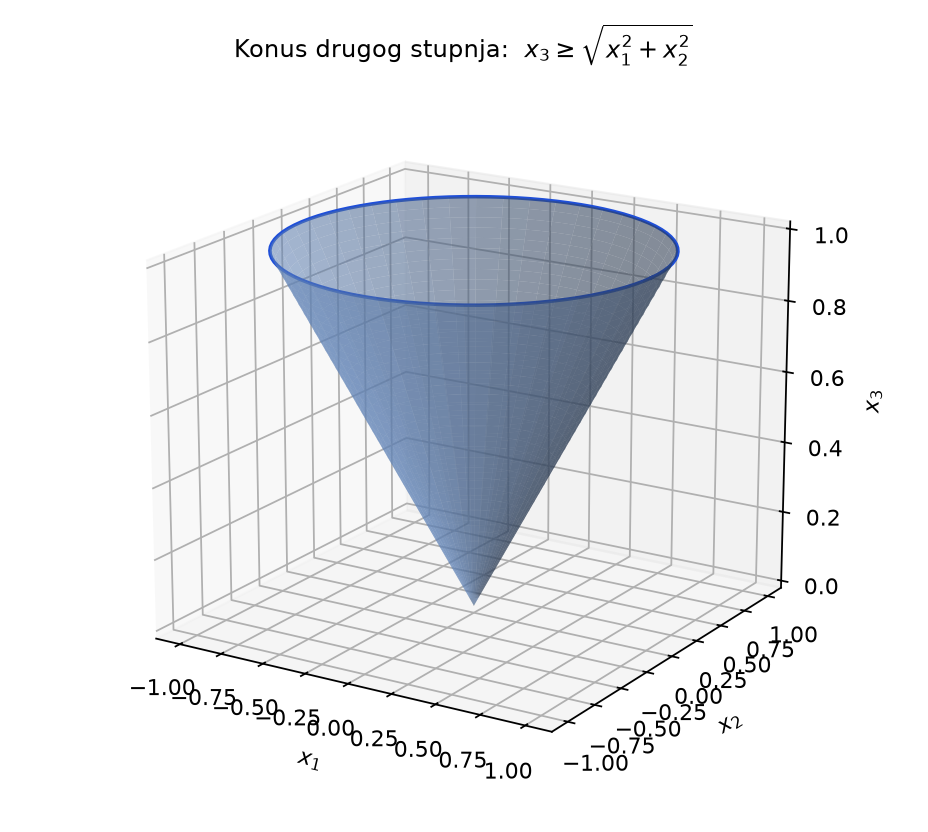
\includegraphics[width=0.56\textwidth]{06-konus.png}
\caption{Konus drugog stupnja u $\R^3$. CQP ograničenje traži da vektor
$(A_ix - b_i)$ leži unutar takvog konusa.}
\end{figure}

\begin{definicija}[Konično kvadratno programiranje (CQP) \str{11}]
\begin{equation}
\label{eq:cqp}
\begin{aligned}
\min \quad & c\T x \\
\uzogr & A_ix - b_i \succeq_K 0, \quad i = 1,\dots,m \\
       & Fx = g
\end{aligned}
\end{equation}
\end{definicija}

\textbf{Alternativna formulacija CQP} \str{12}:
\begin{equation}
\label{eq:cqp-alt}
\begin{aligned}
\min \quad & c\T x \\
\uzogr & \|\tilde A_ix + \tilde b_i\|_2 \le \hat a_i\T x + \hat b_i,
         \quad i = 1,\dots,m \\
       & Fx = g
\end{aligned}
\end{equation}

\emph{Veza dvaju zapisa:} uvjet $y \in K_{SO}$ za vektor
$y = (y_1,\dots,y_{n-1}, y_n)$ glasi $\|(y_1,\dots,y_{n-1})\|_2 \le y_n$.
Ako prvih $n-1$ komponenata bude $\tilde A_ix + \tilde b_i$, a zadnja
$\hat a_i\T x + \hat b_i$, dobiva se točno \eqref{eq:cqp-alt}. \checkmark

\textbf{Dva granična slučaja (sa slajda 12):}
\begin{itemize}
  \item za $\tilde A_i = 0$, CQP se \textbf{reducira u LP}
        (lijeva strana postane $\|\tilde b_i\|_2$, konstanta, pa je
        ograničenje linearno);
  \item za $\hat a_i = 0$, CQP se reducira u \textbf{kvadratno ograničen
        kvadratni program (QCQP)} (engl.\ \emph{quadratically constrained
        quadratic program}).
\end{itemize}

\subsection{Kvadratno ograničen kvadratni program (QCQP)}
\str{13}

\begin{definicija}[QCQP]
\begin{equation}
\begin{aligned}
\min_x \quad & 0{,}5\,x\T P_0x + q_0\T x + r_0 \\
\uzogr & 0{,}5\,x\T P_ix + q_i\T x + r_i \le 0, \quad i = 1,\dots,m \\
       & Fx = g
\end{aligned}
\end{equation}
gdje su $P_i \in \mathbb{S}^n_+$, pa su funkcija cilja i funkcije ograničenja
konveksne funkcije.
\end{definicija}

\textbf{Tvrdnja sa slajda:} kad su sve matrice $P_1,\dots,P_m$ pozitivno
definitne, dozvoljeni skup je \textbf{presjek $m$ elipsoida} i afinog skupa
(definiranog s ograničenjem jednakosti).

\begin{napomena}[usporedba QP i QCQP]
Kod \textbf{QP}-a \eqref{eq:qp} kvadratna je \emph{samo funkcija cilja}, a
ograničenja su linearna --- dozvoljeni skup je politop. Kod \textbf{QCQP}-a su
i ograničenja kvadratna, pa dozvoljeni skup ima \emph{zaobljene} rubove
(presjek elipsoida). To je strogo šira klasa: svaki QP je QCQP (uz
$P_i = 0$), ali ne i obratno.
\end{napomena}

\subsection{Primjer: robusno linearno programiranje}
\label{sec:robusni-lp-cqp}
\str{14--15}

\textbf{Postavka} \str{14}\textbf{.} Promotrimo LP
\[
\min_x c\T x \qquad \uzogr a_i\T x \le b_i, \quad i = 1,\dots,m
\]
i pretpostavimo da su vektori $a_i$ \textbf{nesigurni} u smislu da ne znamo
njihove vrijednosti, već znamo samo da $a_i \in \mathcal{E}_i$.

\textbf{Robusni LP:}
\begin{equation}
\label{eq:robusni-lp}
\min_x c\T x \qquad \uzogr a_i\T x \le b_i \;\;\textbf{za sve } a_i \in \mathcal{E}_i,
\quad i = 1,\dots,m
\end{equation}

\begin{napomena}[što znači „za sve”]
Ovo je \textbf{polu-beskonačno} ograničenje: jedna nejednakost za \emph{svaku}
od beskonačno mnogo mogućih vrijednosti $a_i$. Ne može se izravno predati
rješavaču. Cijeli trik robusnog optimiranja (i poglavlja~\ref{ch:robusno}) je
u tome da se taj beskonačan skup uvjeta zamijeni \textbf{jednim} uvjetom na
najgori slučaj.
\end{napomena}

\textbf{Slučaj elipsoidne nesigurnosti} \str{15}\textbf{.} U slučaju kad su
$\mathcal{E}_i$ elipsoidi:
\[
\mathcal{E}_i = \{\, \bar a_i + P_iu \mid \|u\|_2 \le 1 \,\},
\qquad \bar a_i \in \R^n,\; P_i \in \R^{n\times n} \text{ poznati}
\]
\begin{itemize}
  \item centar elipsoida $\mathcal{E}_i$ je $\bar a_i$;
  \item poluosi su određene \textbf{singularnim vrijednostima} i singularnim
        vektorima matrice $P_i$.
\end{itemize}

\begin{teorem}[Robusni LP kao CQP \str{15}]
Robusni LP je ekvivalentan sljedećem CQP:
\begin{equation}
\label{eq:robusni-lp-cqp}
\min_x c\T x \qquad \uzogr
\bar a_i\T x + \|P_i\T x\|_2 \le b_i, \quad i = 1,\dots,m
\end{equation}
\end{teorem}

\textbf{Zašto} (sa slajda): to slijedi iz toga što je
\[
\sup_{\|u\|_2 \le 1}(\bar a_i + P_iu)\T x
= \bar a_i\T x + \|P_i\T x\|_2
\]

\emph{Raspis (na slajdu nije prikazan).}
\[
(\bar a_i + P_iu)\T x = \bar a_i\T x + (P_iu)\T x
= \bar a_i\T x + u\T P_i\T x
\]
Prvi član ne ovisi o $u$. Drugi je skalarni produkt $\langle u, P_i\T x\rangle$,
koji je po $\|u\|_2 \le 1$ maksimalan kad je $u$ \textbf{u smjeru} $P_i\T x$ i
jedinične duljine: $u^\star = P_i\T x/\|P_i\T x\|_2$. Tada je
\[
u^{\star\top}P_i\T x = \frac{\|P_i\T x\|_2^2}{\|P_i\T x\|_2} = \|P_i\T x\|_2
\]
\checkmark (Ista Cauchy-Schwarzova ideja kao kod Chebyshevljevog centra,
odjeljak~5.5.2.)

\begin{napomena}[tipfeler na slajdu 15]
U izrazu za supremum na slajdu piše
$\sup_{\|u\|_2\le1}(\bar a_i + P_iu)\T = \bar a_ix + \|P_i\T x\|_2$: na lijevoj
strani nedostaje $x$ nakon transponata, a na desnoj nedostaje transponat u
$\bar a_i\T x$. Ispravno je kako je napisano gore.
\end{napomena}

\textbf{Interpretacija:} $\|P_i\T x\|_2$ je \textbf{sigurnosna rezerva} ---
koliko moramo „ostaviti mjesta” da bi ograničenje vrijedilo i za najgori
mogući $a_i$. Što je elipsoid nesigurnosti veći (veći $P_i$), to je rezerva
veća i rješenje konzervativnije.

\begin{figure}[H]
\centering
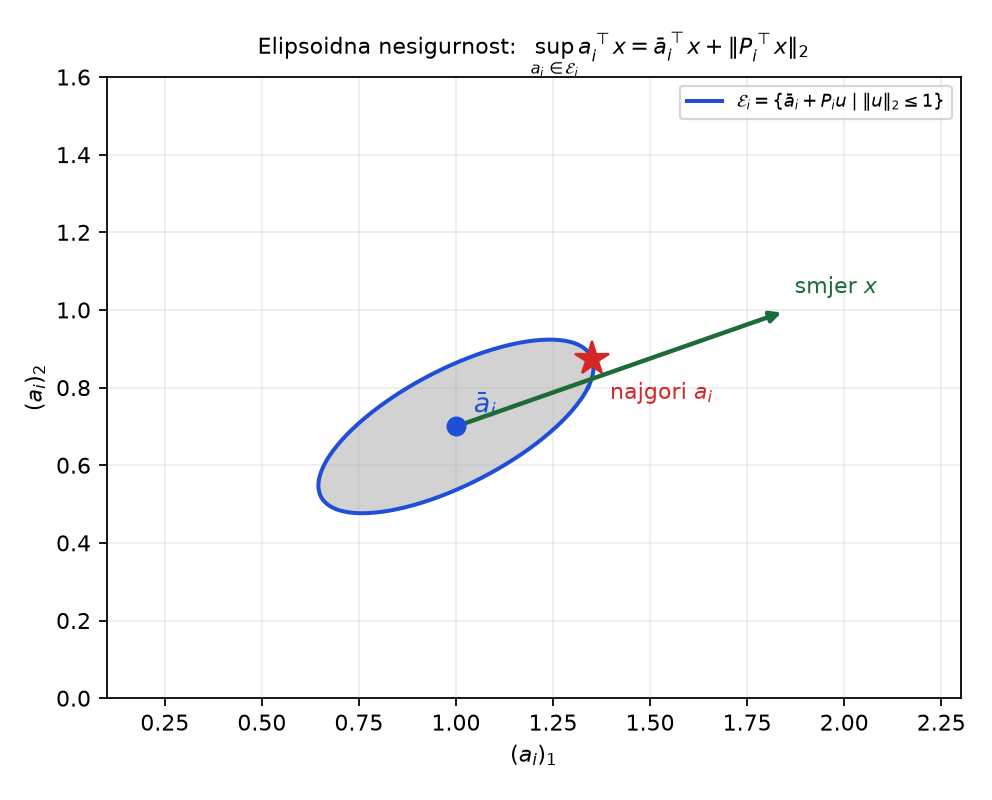
\includegraphics[width=0.70\textwidth]{06-robusni-lp.png}
\caption{Elipsoidni skup nesigurnosti oko $\bar a_i$. Za zadani smjer $x$,
najgori $a_i$ je onaj koji najdalje strši u tom smjeru; njegov doprinos je
$\bar a_i\T x + \|P_i\T x\|_2$.}
\end{figure}

% =====================================================================
\section{Linearne matrične nejednakosti (LMI)}
\label{sec:lmi}
\str{17--22}

\begin{definicija}[Linearna matrična nejednakost \str{17}]
\begin{equation}
\label{eq:lmi}
F(x) = F_0 + x_1F_1 + \dots + x_nF_n \prec 0
\end{equation}
\begin{itemize}
  \item Vektor $x = \begin{pmatrix}x_1 & x_2 & \dots & x_n\end{pmatrix}\T$ je
        vektor projektnih varijabli.
  \item Matrice $F_0, F_1, \dots, F_n$ su \textbf{simetrične} matrice
        ($F_i = F_i\T$), $\to$ $F(x) = F(x)\T$.
  \item $F(x)$ je (matrična) \textbf{afina} funkcija od projektnih varijabli
        $x$ (svaki element od $F(x)$ je afina funkcija od $x$).
\end{itemize}
\end{definicija}

\textbf{Što znači $\prec 0$} (sa slajda):
\begin{align}
F(x) \prec 0
&\Leftrightarrow z\T F(x)z < 0 \text{ za svaki vektor } z \ne 0 \\
&\Leftrightarrow \text{sve svojstvene vrijednosti od } F(x)
   \text{ su negativne} \\
&\Leftrightarrow \text{najveća svojstvena vrijednost od } F(x)
   \text{ je negativna, } \lambda_{\max}(F(x)) < 0
\end{align}

$F(x) \prec G(x)$ znači $F(x) - G(x) \prec 0$ (ekvivalentno za $\preceq$,
$\succ$, $\succeq$). Na sličan način definirane su i matrične nejednadžbe
$F(x) \preceq 0$, $F(x) \succ 0$, $F(x) \succeq 0$ \str{18}.

\subsection{Primjer rastava na standardni oblik}
\str{19--20}

\[
F(x) = \begin{pmatrix}
1 + x_1 & -1 + x_1 + 2x_2 \\
-1 + x_1 + 2x_2 & -3 + x_2
\end{pmatrix}
\]

\textbf{Rastav} \str{20}:
\[
F(x) = \underbrace{\begin{pmatrix}1 & -1 \\ -1 & -3\end{pmatrix}}_{F_0}
     + x_1\underbrace{\begin{pmatrix}1 & 1 \\ 1 & 0\end{pmatrix}}_{F_1}
     + x_2\underbrace{\begin{pmatrix}0 & 2 \\ 2 & 1\end{pmatrix}}_{F_2}
\]

\textbf{Kako se to čita.} Svaki element matrice je afina funkcija od $x$;
grupiraju se po varijablama:
\begin{itemize}
  \item \textbf{konstantni dio} svakog elementa ide u $F_0$: $(1,1)$-element
        ima konstantu $1$, $(1,2)$-element ima $-1$, $(2,2)$-element ima $-3$;
  \item \textbf{koeficijenti uz $x_1$} idu u $F_1$: element $(1,1)$ ima $1$,
        element $(1,2)$ ima $1$, element $(2,2)$ ima $0$;
  \item \textbf{koeficijenti uz $x_2$} idu u $F_2$: element $(1,1)$ ima $0$,
        element $(1,2)$ ima $2$, element $(2,2)$ ima $1$.
\end{itemize}
Sve tri matrice ispadaju simetrične, kao što definicija traži. \checkmark

\subsection{LMI definira konveksan skup}
\str{21}

\begin{teorem}
Linearna matrična nejednadžba definira \textbf{konveksna ograničenja} na $x$ u
smislu da je skup
\[
\Feas := \{\, x \mid F(x) \prec 0 \,\}
\]
konveksan skup. Isto vrijedi i za skupove $\{x \mid F(x) \preceq 0\}$,
$\{x \mid F(x) \succ 0\}$, $\{x \mid F(x) \succeq 0\}$.
\end{teorem}

\textbf{Dokaz (sa slajda).} Za $x_1, x_2 \in \Feas$ i $\alpha \in \R$ vrijedi
\[
F(\alpha x_1 + (1-\alpha)x_2) = \alpha F(x_1) + (1-\alpha)F(x_2) \prec 0.
\]

\emph{Dopuna dokaza (slajd je sažet).} Prva jednakost vrijedi jer je $F$ afina
i $\alpha + (1-\alpha) = 1$ --- konstantni član $F_0$ se „ne razdvoji”. Zadnja
nejednakost vrijedi za $\alpha \in [0,1]$: tada su oba koeficijenta
nenegativna, a konus negativno definitnih matrica je konveksan konus (isti
argument kao za $\mathbb{S}^n_+$ u odjeljku \str{7}). \checkmark

\textbf{Dodatna tvrdnja sa slajda:} funkcija
$f : x \mapsto \lambda_{\max}(F(x))$ je \textbf{konveksna} funkcija.

\subsection{Matrične varijable}
\str{22}

Iako se svaka LMN može svesti na standardni oblik \eqref{eq:lmi}, često se
projektne varijable ostavljaju kao \textbf{matrice} u zapisu LMN-a.

\textbf{Primjer sa slajda:}
\[
A\T P + PA \prec 0
\]
je LMN s $A$ zadanom kvadratnom matricom i $P$ simetričnom kvadratnom
matricom koja je projektna varijabla (\textbf{svi elementi ove matrice su
projektne varijable}).

\textbf{Uočite da je $A\T P + PA$ simetrična matrica.}

\emph{Provjera:} $(A\T P + PA)\T = P\T A + A\T P\T = PA + A\T P$ (jer je
$P = P\T$) $= A\T P + PA$. \checkmark

\begin{napomena}[koliko varijabli zapravo ima]
Ako je $P$ simetrična $n\times n$ matrica, ona ima $n(n+1)/2$ nezavisnih
elemenata --- toliko je i projektnih varijabli. Za $n = 4$ to je $10$. Zapis s
matričnom varijablom je samo kraći način pisanja; standardni oblik
\eqref{eq:lmi} dobio bi se izborom baze simetričnih matrica.

Ovu konkretnu LMN, $A\T P + PA \prec 0$, srest ćemo u
poglavlju~\ref{ch:dinamicki} kao \textbf{Ljapunovljevu nejednakost} --- uvjet
stabilnosti dinamičkog sustava.
\end{napomena}

% =====================================================================
\section{Semidefinitno programiranje (SDP)}
\str{23--25}

\begin{definicija}[Općenit semidefinitan program \str{23}]
Neka su $F_1,\dots,F_m$ funkcije koje mapiraju $X$ u skup simetričnih matrica.
Općenit SDP problem je
\begin{equation}
\label{eq:sdp}
\begin{aligned}
\min_x \quad & f(x) \\
\uzogr & x \in X, \quad F_1(x) \preceq 0,\; \dots,\; F_m(x) \preceq 0
\end{aligned}
\end{equation}
\end{definicija}

\textbf{Tvrdnje sa slajda:}

\begin{itemize}
  \item Ovakva formulacija uključuje probleme \textbf{nelinearnog
        programiranja} kao poseban slučaj.
  \item Ovo je \textbf{konveksan SDP} ako su $f, F_1,\dots,F_m$ konveksne
        funkcije.
  \item Ovo je \textbf{optimizacijski problem s linearnim matričnim
        nejednakostima} (engl.\ \emph{Linear matrix inequality (LMI)
        optimization problem}) ili \textbf{linearan SDP} ako su
        $f, F_1,\dots,F_m$ afine funkcije.
\end{itemize}

\subsection{Blok-dijagonalna svojstva}
\str{24--25}

\begin{teorem}[Dijagonalni blokovi \str{24}]
Neka je kvadratna simetrična matrica $A$ particionirana na sljedeći način
\[
A = \begin{pmatrix}
A_{11} & \dots & A_{1m} \\
\vdots & \ddots & \vdots \\
A_{m1} & \dots & A_{mm}
\end{pmatrix} \prec 0
\]
gdje su matrice na dijagonali $A_{11},\dots,A_{mm}$ kvadratne. Tada
$A \prec 0$ implicira $A_{11} \prec 0,\; \dots,\; A_{mm} \prec 0$.
\end{teorem}

\textbf{Dokaz.} Na ploči. \emph{(Tako stoji na slajdu; dokaz nije zapisan.)}

\begin{napomena}[ideja dokaza]
Slajd upućuje na ploču, pa ga ne prepisujem. Skica koja slijedi izravno iz
definicije: uzmite vektor $z$ koji je nula svugdje osim u bloku $k$, gdje je
jednak proizvoljnom $w \ne 0$. Tada je $z\T Az = w\T A_{kk}w$, a lijeva strana
je $< 0$ po pretpostavci --- dakle $A_{kk} \prec 0$.
\end{napomena}

\textbf{Skup LMN-ova kao jedna LMN} \str{25}\textbf{.} Skup pojedinačnih
LMN-ova može se zapisati kao \emph{jedna} LMN:
\[
F_1(x) \prec 0,\; \dots,\; F_k(x) \prec 0
\qquad\text{je isto kao i}\qquad
F(x) = \begin{pmatrix}
F_1(x) & 0 & \dots & 0 \\
0 & \ddots & & 0 \\
0 & 0 & \dots & F_k(x)
\end{pmatrix} \prec 0
\]

\textbf{Primjer sa slajda:}
\[
P \succ 0, \quad A\T P + PA \prec 0
\qquad\Longleftrightarrow\qquad
\begin{pmatrix} -P & 0 \\ 0 & A\T P + PA \end{pmatrix} \prec 0
\]

\emph{Zašto:} $P \succ 0$ je isto što i $-P \prec 0$. Blok-dijagonalna matrica
je negativno definitna točno onda kad je svaki dijagonalni blok negativno
definitan (prethodni teorem daje jedan smjer; obrat je jednako lak).

\textbf{Praktična vrijednost:} rješavači SDP-a očekuju \emph{jednu} matričnu
nejednakost. Ovim se trikom proizvoljno mnogo uvjeta spakira u jedan.

% =====================================================================
\section{Transformacija kongruencije}
\label{sec:kongruencija}
\str{26}

\begin{definicija}[Kongruencija]
Kvadratne matrice $A$ i $B$ su \textbf{kongruentne} ako postoji regularna
kvadratna matrica $T$ takva da je
\[
T\T AT = B.
\]
\textbf{Transformacija kongruencije} s matricom $T$: $A \to T\T AT$.
\end{definicija}

\begin{teorem}[Kongruencija čuva definitnost]
Neka je $T$ regularna kvadratna matrica. Tada vrijedi
\[
\begin{aligned}
A \prec 0 &\;\to\; T\T AT \prec 0 &\qquad
A \succ 0 &\;\to\; T\T AT \succ 0 \\
A \preceq 0 &\;\to\; T\T AT \preceq 0 &\qquad
A \succeq 0 &\;\to\; T\T AT \succeq 0
\end{aligned}
\]
\end{teorem}

\textbf{Pitanja sa slajda:} \emph{Zašto? Što ako $T$ nije regularna? Ili ako je
„visoka” matrica, ali stupci jesu/nisu linearno nezavisni?}

\textbf{Odgovori} (slajd postavlja pitanja, ali ne daje odgovore; niže slijedi
izvod iz same definicije definitnosti):

\emph{Zašto vrijedi:} za proizvoljan $z \ne 0$ stavimo $w := Tz$. Tada je
\[
z\T(T\T AT)z = (Tz)\T A(Tz) = w\T Aw
\]
Ako je $T$ regularna, $z \ne 0$ povlači $w \ne 0$, pa je $w\T Aw < 0$ po
pretpostavci $A \prec 0$. Dakle $z\T(T\T AT)z < 0$ za svaki $z \ne 0$.
\checkmark

\emph{Ako $T$ nije regularna:} postoji $z \ne 0$ s $Tz = 0$, pa je
$z\T(T\T AT)z = 0$. Stroga nejednakost se \textbf{gubi} --- ostaje samo
$T\T AT \preceq 0$. Nestroge relacije ($\preceq$, $\succeq$) preživljavaju i
bez regularnosti.

\emph{Ako je $T$ „visoka”} ($k \times n$, $k > n$): tada je $T\T AT$ dimenzija
$n \times n$. Presudno je jesu li \textbf{stupci} od $T$ linearno nezavisni:
ako jesu, $Tz = 0$ povlači $z = 0$, pa stroga definitnost \emph{ostaje}; ako
nisu, opet se gubi na $\preceq$.

% =====================================================================
\section{Schurov komplement}
\label{sec:schur}
\str{27--28}

\begin{teorem}[Pravilo Schurovog komplementa]
Simetrična matrica
$M = \begin{pmatrix} M_{11} & M_{12} \\ M_{21} & M_{22}\end{pmatrix}$
je \textbf{negativno definitna}

\medskip
\textbf{ako i samo ako}\quad
$M_{11} \prec 0$ \quad i \quad $M_{22} - M_{21}M_{11}^{-1}M_{12} \prec 0$

\medskip
\textbf{ako i samo ako}\quad
$M_{22} \prec 0$ \quad i \quad $M_{11} - M_{12}M_{22}^{-1}M_{21} \prec 0$

\medskip
Matrice $S_1 := M_{22} - M_{21}M_{11}^{-1}M_{12}$ i
$S_2 := M_{11} - M_{12}M_{22}^{-1}M_{21}$ zovu se \textbf{Schurovi
komplementi}.
\end{teorem}

\textbf{Dokaz (sa slajda 28).} Lijeva strana jednakosti
\[
\begin{pmatrix} I & 0 \\ -M_{11}^{-1}M_{12} & I \end{pmatrix}\T
\begin{pmatrix} M_{11} & M_{12} \\ M_{21} & M_{22} \end{pmatrix}
\begin{pmatrix} I & 0 \\ -M_{11}^{-1}M_{12} & I \end{pmatrix}
= \begin{pmatrix} M_{11} & 0 \\ 0 & S_1 \end{pmatrix}
\]
je oblika $T\T MT$ gdje je $T$ nesingularna matrica (transformacija
kongruencije).

\textbf{Kako dokaz funkcionira, u tri rečenice.} Matrica $T$ je donje
trokutasta s jedinicama na dijagonali, pa je uvijek regularna --- transformacija
kongruencije dakle \textbf{čuva definitnost} (odjeljak~\ref{sec:kongruencija}).
Rezultat transformacije je \emph{blok-dijagonalna} matrica, a ona je negativno
definitna točno onda kad su oba bloka negativno definitna \str{24}. Time je
$M \prec 0 \Leftrightarrow M_{11}\prec0$ i $S_1 \prec 0$. $\blacksquare$

\begin{napomena}[zašto je Schurov komplement najvažniji alat SDP-a]
Schurov komplement je \textbf{stroj za pretvaranje nelinearnih uvjeta u
linearne matrične nejednakosti}. Uvjet
\[
M_{22} - M_{21}M_{11}^{-1}M_{12} \prec 0
\]
je \emph{nelinearan} u nepoznanicama (sadrži inverz i umnožak), ali je
ekvivalentan uvjetu $M \prec 0$, koji je \textbf{afin} u istim nepoznanicama.

Zato: kad god u problemu vidite kvadratni član ili inverz, pokušajte ga
„razmotati” Schurovim komplementom u LMN. Upravo tako nastaje SDP formulacija
u sljedećem odjeljku, a i cijelo poglavlje~\ref{ch:dinamicki}.
\end{napomena}

% =====================================================================
\section{Primjer: minimizacija norme matrice}
\str{29}

\textbf{Zadatak.} Minimizacija 2.\ inducirane norme matrice:
\[
\min_x \; \|A(x)\|_2 = \big(\lambda_{\max}(A(x)\T A(x))\big)^{1/2}
\]
gdje je $\lambda_{\max}$ najveća svojstvena vrijednost matrice.

\textbf{Ključni lanac ekvivalencija:}
\begin{equation}
\label{eq:norma-lmi}
\|A\|_2 \le t
\quad\Leftrightarrow\quad
A\T A \preceq t^2I,\; t \ge 0
\quad\Leftrightarrow\quad
\begin{pmatrix} tI & A \\ A\T & tI \end{pmatrix} \succeq 0
\end{equation}

pa je ekvivalentan SDP problem
\[
\begin{aligned}
\min_{t,x} \quad & t \\
\uzogr & \begin{pmatrix} tI & A(x) \\ A(x)\T & tI \end{pmatrix} \succeq 0
\end{aligned}
\]

\textbf{Objašnjenje lanca:}

\begin{itemize}
  \item \emph{Prva ekvivalencija:} po definiciji je $\|A\|_2^2 =
        \lambda_{\max}(A\T A)$, pa $\|A\|_2 \le t$ znači da su sve svojstvene
        vrijednosti od $A\T A$ najviše $t^2$ --- a to je upravo
        $A\T A \preceq t^2 I$.
  \item \emph{Druga ekvivalencija:} to je \textbf{Schurov komplement}
        primijenjen na blok-matricu. Uz $M_{11} = tI \succ 0$ (za $t>0$),
        uvjet $M \succeq 0$ svodi se na
        \[
        M_{22} - M_{21}M_{11}^{-1}M_{12} = tI - A\T(tI)^{-1}A
        = tI - \tfrac1t A\T A \succeq 0
        \]
        Množenjem s $t > 0$: $t^2I - A\T A \succeq 0$, tj.\
        $A\T A \preceq t^2I$. \checkmark
\end{itemize}

\textbf{Poanta:} cilj je bio \emph{nelinearna} funkcija (korijen najveće
svojstvene vrijednosti), a rezultat je \textbf{linearan} SDP --- cilj $t$ je
linearan, a ograničenje je afino u $(t,x)$ ako je $A(x)$ afina. To je isti
trik s pomoćnom varijablom kao kod $\infty$-norme
(odjeljak~2.20.2), samo u matričnom svijetu.

% =====================================================================
\section{Hijerarhija: LP $\subset$ CQP $\subset$ SDP}
\str{30--31}

\subsection{LP kao podskup od SDP}
\str{30}

\[
\begin{aligned}
\text{\textbf{LP}} \qquad
\min_x \; & c\T x \\
\uzogr & Ax \le b \\
& Gx = h
\end{aligned}
\qquad\Updownarrow\qquad
\begin{aligned}
\text{\textbf{linearni SDP}} \qquad
\min_x \; & c\T x \\
\uzogr & \diag(Ax - b) \preceq 0 \\
& Gx = h
\end{aligned}
\]

\emph{Zašto:} $\diag(v)$ je dijagonalna matrica s elementima vektora $v$ na
dijagonali. Njezine svojstvene vrijednosti \emph{jesu} ti elementi, pa je
$\diag(v) \preceq 0$ točno onda kad su svi $v_i \le 0$ --- dakle isto što i
$v \le 0$ po komponentama. \checkmark

\subsection{CQP kao podskup od SDP}
\str{31}

\[
\begin{aligned}
\text{\textbf{CQP}} \qquad
\min \; & f\T x \\
\uzogr & \|A_ix + b_i\|_2 \le c_i\T x + d_i, \; i = 1,\dots,m \\
& Gx = h
\end{aligned}
\]
\[
\Updownarrow
\]
\[
\begin{aligned}
\text{\textbf{linearni SDP}} \qquad
\min_x \; & f\T x \\
\uzogr & \begin{pmatrix}
(c_i\T x + d_i)I & A_ix + b_i \\
(A_ix + b_i)\T & c_i\T x + d_i
\end{pmatrix} \succeq 0 \\
& Gx = h
\end{aligned}
\]

\emph{Zašto:} opet Schurov komplement. Označimo $y := A_ix + b_i$ i
$s := c_i\T x + d_i$. Uz $M_{11} = sI \succ 0$, uvjet $M \succeq 0$ svodi se na
\[
s - y\T(sI)^{-1}y = s - \frac{\|y\|_2^2}{s} \ge 0
\]
što je (za $s > 0$) isto što i $s^2 \ge \|y\|_2^2$, tj.\ $\|y\|_2 \le s$.
\checkmark

\begin{teorem}[Zaključak]
\[
\text{LP} \;\subset\; \text{CQP} \;\subset\; \text{SDP}
\]
Svaki LP je CQP, svaki CQP je SDP. SDP je najšira od triju klasa i za nju
postoje učinkoviti rješavači (metode unutrašnje točke).
\end{teorem}

\begin{napomena}[praktični savjet]
Ako uspijete problem zapisati kao LP --- učinite to, jer je najbrži. Ako ne, pa
uspijete kao CQP --- i to je odlično. Ako ni to, ali uspijete kao SDP --- problem
je i dalje \emph{rješiv} i to pouzdano. Tek ako ni SDP ne prolazi, ulazite u
područje općeg (ili nekonveksnog) optimiranja gdje nema jamstava.
\end{napomena}

% =====================================================================
\section{Vježbe 4: geometrijski problemi --- klasifikacija}
\label{sec:klasifikacija}
\str{V4:31--41}

Ovo je zaključni dio Vježbi 4 i najprirodnije mjesto za njega je ovdje: problem
robusne klasifikacije je QP koji se izvodi \emph{dualnošću}, i vodi izravno na
poznati \emph{support vector} klasifikator.

\subsection{Linearna klasifikacija}
\str{V4:32}

\begin{definicija}[Linearna klasifikacija]
\textbf{Cilj:} separirati (razdvojiti) dva zadana skupa točaka
$\{x_1,\dots,x_N\}$, $\{y_1,\dots,y_M\}$ s \textbf{hiperravninom}
($x_i \in \R^n$, $y_j \in \R^n$) $\to$ pronaći $a \in \R^n$ i $b \in \R$ takve
da vrijedi
\[
a\T x_i + b > 0,\; i = 1,\dots,N, \qquad
a\T y_j + b < 0,\; j = 1,\dots,M.
\]
\end{definicija}

\textbf{Normalizacija} (sa slajda). Budući da su gore predstavljene
nejednakosti \textbf{homogene} u $a$ i $b$ (ako vrijedi $a\T x_i + b > 0$, onda
vrijedi i $\tilde a\T x_i + \tilde b > 0$, gdje su $\tilde a = \alpha a$,
$\tilde b = \alpha b$ za $\alpha > 0$), možemo problem ekvivalentno formulirati
kao: nađi $a$ i $b$ takve da vrijedi
\begin{equation}
\label{eq:klasifikacija}
a\T x_i + b \ge 1,\; i = 1,\dots,N, \qquad
a\T y_j + b \le -1,\; j = 1,\dots,M.
\end{equation}

\textbf{Ovo je skup linearnih nejednakosti u $a$ i $b$, pa se problem svodi na
LP.}

\begin{napomena}[zašto smijemo staviti baš $\pm1$]
Stroge nejednakosti ($> 0$) nezgodne su za rješavače --- optimum bi bio na rubu
koji nije uključen. Skaliranjem se strogi uvjet pretvara u nestrogi s
„rezervom”: ako postoji rješenje s $a\T x_i + b > 0$ za sve $i$, onda je
najmanja od tih vrijednosti neki $\varepsilon > 0$, pa dijeljenjem cijelog para
$(a,b)$ s $\varepsilon$ dobivamo $\ge 1$. Vrijednost $1$ je proizvoljna --- bitno
je samo da je pozitivna i fiksna.
\end{napomena}

\subsection{Robusna linearna klasifikacija}
\str{V4:33}

\textbf{Motivacija.} Ako se skupovi mogu razdvojiti, obično postoji
\emph{beskonačno mnogo} hiperravnina koje to čine. Koju odabrati? Onu koja je
\textbf{najdalje} od obiju skupina --- najotporniju na šum u podacima.

\textbf{Euklidska udaljenost između hiperravnina}
\[
H_1 := \{\, z \mid a\T z + b = 1 \,\}, \qquad
H_2 := \{\, z \mid a\T z + b = -1 \,\}
\]
je
\[
\dist(H_1, H_2) = \min_{z_1,z_2}\{\, \|z_1 - z_2\|_2 \mid
z_1 \in H_1,\; z_2 \in H_2 \,\}
\]

\textbf{Problem robusne linearne klasifikacije:}
\begin{equation}
\label{eq:robusna-klasifikacija}
\begin{aligned}
\max_{a,b} \quad & \dist(H_1, H_2) \\
\uzogr & a\T x_i + b \ge 1, && i = 1,\dots,N \\
       & a\T y_j + b \le -1, && j = 1,\dots,M
\end{aligned}
\end{equation}

\subsection{Izračun udaljenosti dualnošću}
\str{V4:34--38}

Cijeli je posao izračunati $\dist(H_1,H_2)$ kao funkciju od $a$. Slajdovi to
rade \textbf{Lagrangeovom dualnošću} --- lijep primjer primjene
poglavlja~\ref{ch:dualnost}.

\textbf{Dva primarna problema} \str{V4:34}:

\[
\begin{aligned}
\text{\textbf{Primarni problem 1}} \\
\min_{z_1,z_2} \; & \|z_1 - z_2\|_2 \\
\uzogr & a\T z_1 + b - 1 = 0 \\
& a\T z_2 + b + 1 = 0
\end{aligned}
\qquad\Rightarrow\qquad
\begin{aligned}
\text{\textbf{Primarni problem 2}} \\
\min_{z_1,z_2} \; & \|z_1 - z_2\|_2^2 = (z_1-z_2)\T(z_1-z_2) \\
\uzogr & a\T z_1 + b - 1 = 0 \\
& a\T z_2 + b + 1 = 0
\end{aligned}
\]

(Kvadriranje norme je uobičajeni trik iz odjeljka~2.20.2.)

\textbf{Jaka dualnost vrijedi. Lagrangian (za primarni problem 2)}
\str{V4:35}:
\begin{align}
L(\lambda_1,\lambda_2,z_1,z_2)
&= (z_1-z_2)\T(z_1-z_2) + \lambda_1(a\T z_1 + b - 1)
   + \lambda_2(a\T z_2 + b + 1) \\
&= (z_1-z_2)\T(z_1-z_2)
   + \begin{pmatrix}\lambda_1a\T & \lambda_2a\T\end{pmatrix}
     \begin{pmatrix}z_1\\z_2\end{pmatrix}
   + (\lambda_1+\lambda_2)b + (\lambda_2 - \lambda_1)
\end{align}

\textbf{Korak 1 --- kada je dualna funkcija $-\infty$} \str{V4:36}\textbf{.}
Uočimo da za $\lambda_1 + \lambda_2 \ne 0$ imamo
$\ell(\lambda_1,\lambda_2) = -\infty$, jer možemo uvijek izabrati
$z_1 = z_2 = z$, pa je $Q = 0$ i $L = (\lambda_1+\lambda_2)a\T z$, te za svaki
$a \ne 0$ izborom $z$ možemo $L$ načiniti proizvoljno malim.

\emph{(Oznake $Q$ i $L$ sa slajda: $Q$ je kvadratni član
$(z_1-z_2)\T(z_1-z_2)$, $L$ je linearni član.)}

\textbf{Korak 2 --- stacionarnost za $\lambda_1 = \lambda$,
$\lambda_2 = -\lambda$} \str{V4:36}\textbf{.} Za $\lambda_1 + \lambda_2 = 0$
infimum se postiže kad gradijent Lagrangiana po primarnim varijablama
$(z_1,z_2)$ izjednačimo s nulom:
\[
2\begin{pmatrix} I & -I \\ -I & I\end{pmatrix}
\begin{pmatrix}z_1\\z_2\end{pmatrix}
+ \begin{pmatrix}\lambda a \\ -\lambda a\end{pmatrix} = 0
\quad\Longrightarrow\quad
(z_1^\star - z_2^\star) = -\tfrac12\lambda a
\]

\emph{Raspis:} gornji blok jednadžbe glasi $2(z_1 - z_2) + \lambda a = 0$, pa je
$z_1 - z_2 = -\lambda a/2$. (Donji blok daje istu jednadžbu s obrnutim
predznakom --- sustav je singularan, jer $L$ ovisi samo o razlici $z_1 - z_2$.)
\checkmark

\textbf{Korak 3 --- dualna funkcija} \str{V4:37}\textbf{.} Za
$\lambda_1 = \lambda$, $\lambda_2 = -\lambda$ imamo
\[
L(\lambda_1,\lambda_2,z_1,z_2)
= \underbrace{(z_1-z_2)\T(z_1-z_2)}_{Q}
+ \underbrace{\lambda a\T(z_1-z_2)}_{L} - 2\lambda
\]
(članovi s $b$ se pokrate jer je $\lambda_1 + \lambda_2 = 0$, a
$\lambda_2 - \lambda_1 = -2\lambda$).

Uvrštavanjem $(z_1 - z_2) = -\tfrac12\lambda a$:
\[
\ell(\lambda,-\lambda) = -\tfrac14 a\T a\,\lambda^2 - 2\lambda
\]

\emph{Raspis uvrštavanja:}
\begin{align}
Q &= \left(-\tfrac12\lambda a\right)\T\left(-\tfrac12\lambda a\right)
   = \tfrac14\lambda^2 a\T a \\
L &= \lambda a\T\left(-\tfrac12\lambda a\right) = -\tfrac12\lambda^2 a\T a \\
Q + L - 2\lambda
  &= \tfrac14\lambda^2a\T a - \tfrac12\lambda^2a\T a - 2\lambda
   = -\tfrac14 a\T a\,\lambda^2 - 2\lambda \quad\checkmark
\end{align}

\textbf{Korak 4 --- maksimizacija po $\lambda$.}
$\max_\lambda \ell(\lambda,-\lambda)$ se postiže za
\[
\lambda^\star = -4\,\frac{1}{a\T a} = -\frac{4}{\|a\|_2^2}
\]

\emph{Raspis:} $\dfrac{\dd\ell}{\dd\lambda} = -\tfrac12 a\T a\,\lambda - 2 = 0
\Rightarrow \lambda = -\dfrac{4}{a\T a}$. \checkmark

\textbf{Korak 5 --- optimalna vrijednost dualnog problema} za primarni problem 2:
\[
d^\star = -\tfrac14 a\T a(\lambda^\star)^2 - 2\lambda^\star
= \frac{4}{a\T a} = \frac{4}{\|a\|_2^2}
\]

\emph{Raspis:}
\[
-\tfrac14 a\T a\cdot\frac{16}{(a\T a)^2} - 2\cdot\left(-\frac{4}{a\T a}\right)
= -\frac{4}{a\T a} + \frac{8}{a\T a} = \frac{4}{a\T a} \quad\checkmark
\]

\textbf{Korak 6 --- povratak na primarni problem 1} \str{V4:38}\textbf{.}
Optimalna vrijednost dualnog problema $=$ optimalna vrijednost primarnog
problema 2 (jaka dualnost):
\[
d^\star = 4/\|a\|_2^2 = p_2^\star
\]
Budući da je problem 2 kvadrirana verzija problema 1, vrijedi
\[
p_1^\star = \sqrt{p_2^\star} = \sqrt{4/\|a\|_2^2} = \frac{2}{\|a\|_2}
\]

\begin{napomena}[tipfeler na slajdu V4:38]
Na slajdu je napisano $p_1^\star = \sqrt{p_1^\star} = \sqrt{4/\|a\|_2^2}$ ---
pod korijenom treba stajati $p_2^\star$, ne $p_1^\star$. Rezultat
$2/\|a\|_2$ je ispravan.
\end{napomena}

\begin{teorem}[Margina]
\[
\dist(H_1, H_2) = \frac{2}{\|a\|_2}
\]
\end{teorem}

\subsection{Konačna QP formulacija}
\str{V4:39}

Budući da je $\dist(H_1,H_2) = 2/\|a\|_2$, maksimizacija udaljenosti je isto
što i \emph{minimizacija} $\|a\|_2$:
\[
\begin{aligned}
\max_{a,b} \; & \dist(H_1,H_2) \\
& a\T x_i + b \ge 1, \; i = 1,\dots,N \\
& a\T y_j + b \le -1, \; j = 1,\dots,M
\end{aligned}
\qquad\Longleftrightarrow\qquad
\begin{aligned}
\min_{a,b} \; & \tfrac12\|a\|_2^2 \\
& a\T x_i + b \ge 1, \; i = 1,\dots,N \\
& a\T y_j + b \le -1, \; j = 1,\dots,M
\end{aligned}
\]

\textbf{Problem robusne linearne klasifikacije formuliran je kao konveksan
QP.}

\emph{Zašto smijemo kvadrirati i staviti $\tfrac12$:} $2/\|a\|_2$ je najveće
kad je $\|a\|_2$ najmanje; kvadriranje i množenje pozitivnom konstantom ne
mijenjaju minimizator. Faktor $\tfrac12$ je konvencija koja pojednostavljuje
gradijent ($\nabla\tfrac12\|a\|^2 = a$).

\begin{figure}[H]
\centering
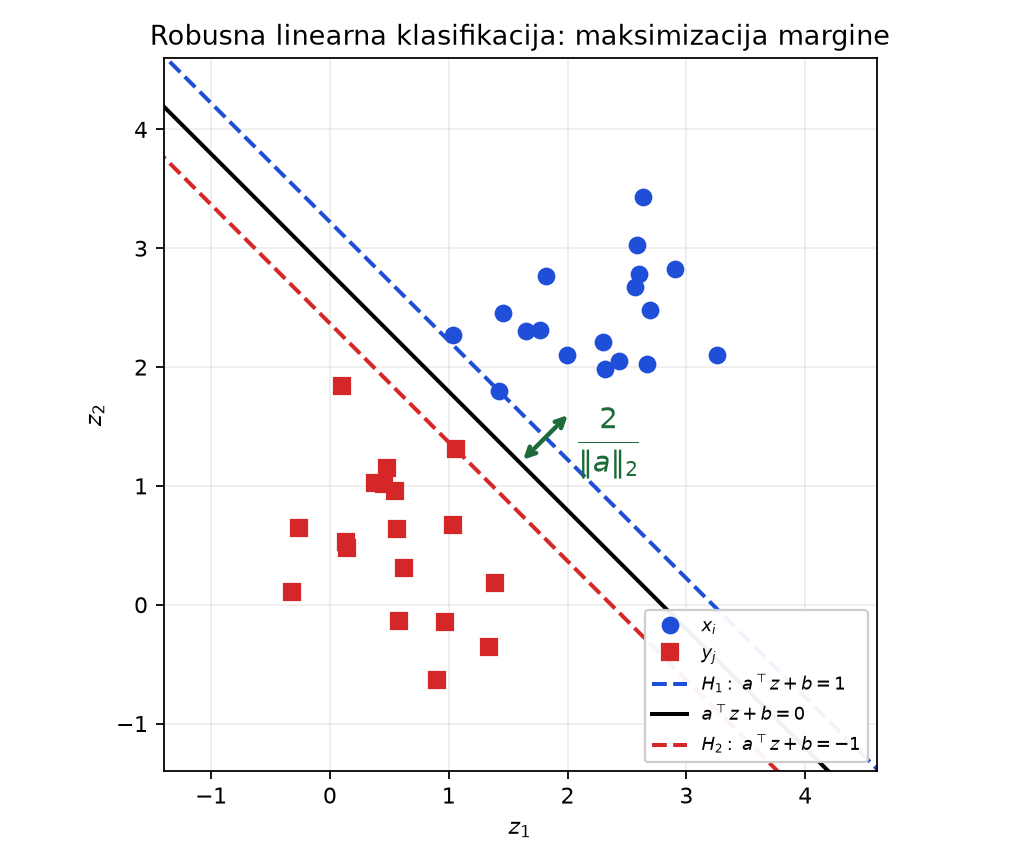
\includegraphics[width=0.72\textwidth]{06-klasifikacija.png}
\caption{Robusna linearna klasifikacija. Traži se hiperravnina s najširim
pojasom između $H_1$ i $H_2$; širina pojasa je $2/\|a\|_2$, pa se maksimizacija
margine svodi na minimizaciju $\|a\|_2$.}
\end{figure}

\begin{crtanje}[margina klasifikatora]
\textbf{Korak 1.} Nacrtajte osi $z_1$, $z_2$, jednako mjerilo. Ucrtajte dvije
skupine točaka --- npr.\ krugove gore desno i kvadrate dolje lijevo.

\textbf{Korak 2 --- razdjelna hiperravnina.} Povucite pravac koji ih razdvaja.
To je skup $\{z \mid a\T z + b = 0\}$. Vektor $a$ je okomit na njega
(odjeljak~\ref{sec:hiperravnine}).

\textbf{Korak 3 --- dvije margine.} Povucite dva pravca paralelna s njim: $H_1$
kroz najbližu točku prve skupine i $H_2$ kroz najbližu točku druge. To su
$a\T z + b = 1$ i $a\T z + b = -1$.

\textbf{Korak 4 --- margina.} Nacrtajte dvosmjernu strelicu okomito između
$H_1$ i $H_2$. Njezina duljina je $2/\|a\|_2$.

\emph{Zašto baš to:} pomak od $H_2$ do $H_1$ u smjeru $a/\|a\|_2$ mijenja
vrijednost $a\T z + b$ za $\|a\|_2$ po jedinici duljine; treba je promijeniti
za $1 - (-1) = 2$, dakle prijeđena udaljenost je $2/\|a\|_2$. \checkmark

\textbf{Korak 5 --- što graf znači.} Manji $\|a\|$ znači \emph{širu} marginu.
Zato minimizacija $\tfrac12\|a\|_2^2$ uz zadana ograničenja daje klasifikator
koji je najotporniji na pomake podataka. Točke koje leže \emph{točno} na $H_1$
ili $H_2$ zovu se \textbf{potporni vektori} --- samo one određuju rješenje; sve
ostale mogu se pomicati bez ikakvog učinka (njihova ograničenja su neaktivna,
pa im je $\mu = 0$, po komplementarnosti iz poglavlja~\ref{ch:uvjeti}).
\end{crtanje}

\subsection{Aproksimativna linearna klasifikacija}
\str{V4:40--41}

\textbf{Problem.} Kad skupovi točaka \textbf{ne mogu} biti odvojeni
hiperravninom (ne postoji egzaktna linearna klasifikacija), ograničenja
\eqref{eq:klasifikacija} nemaju rješenje. Rješenje: dopustiti kršenje, ali ga
kazniti.

\textbf{LP formulacija} \str{V4:40}:
\begin{equation}
\begin{aligned}
\min_{a,b,u,v} \quad & \mathbf{1}\T u + \mathbf{1}\T v \\
\uzogr & a\T x_i + b \ge 1 - u_i, && i = 1,\dots,N \\
       & a\T y_j + b \le -(1 - v_j), && j = 1,\dots,M \\
       & u \ge 0, \quad v \ge 0
\end{aligned}
\end{equation}

\textbf{Ovo je LP.} Ekvivalentno minimizaciji sume „narušenosti” originalnih
ograničenja.

\textbf{QP formulacija --- \emph{support vector classifier}} \str{V4:41}:
\begin{equation}
\label{eq:svc}
\begin{aligned}
\min_{a,b,u,v} \quad & \|a\|_2 + \gamma\big(\mathbf{1}\T u + \mathbf{1}\T v\big) \\
\uzogr & a\T x_i + b \ge 1 - u_i, && i = 1,\dots,N \\
       & a\T y_j + b \le -(1 - v_j), && j = 1,\dots,M \\
       & u \ge 0, \quad v \ge 0
\end{aligned}
\end{equation}

\textbf{Ovo je QP.} \emph{Izborom vrijednosti $\gamma$ radi se kompromis između
robusnosti i klasifikacijske greške.}

\textbf{Kako čitati varijable $u$ i $v$.} $u_i$ je „koliko je $i$-ta točka
prve skupine \emph{prekršila}” svoj uvjet:
\begin{itemize}
  \item $u_i = 0$: točka je ispravno klasificirana i izvan margine;
  \item $0 < u_i < 1$: točka je unutar margine, ali na ispravnoj strani;
  \item $u_i > 1$: točka je \textbf{pogrešno} klasificirana.
\end{itemize}
Zbroj $\mathbf{1}\T u + \mathbf{1}\T v$ je ukupna „mjera greške”.

\begin{napomena}[uloga $\gamma$ --- opet Pareto kompromis]
Ovo je ista struktura kao regularizirana aproksimacija
(odjeljak~\ref{sec:regularizacija}): dva suprotstavljena cilja, skalarizirana
težinom $\gamma$.
\begin{itemize}
  \item mali $\gamma$: dominira $\|a\|_2$, dakle \textbf{široka margina}, ali se
        tolerira više grešaka;
  \item velik $\gamma$: dominira kazna za greške, dakle \textbf{malo grešaka},
        ali uska margina i osjetljivost na šum.
\end{itemize}
Formulacija \eqref{eq:svc} je klasični \emph{support vector machine} --- jedan od
najpoznatijih algoritama strojnog učenja, a kao što vidite, to je samo QP.
\end{napomena}

\begin{napomena}[tipfeler na slajdovima V4:40--41]
U ograničenju za drugu skupinu na slajdu piše $-(1 - v_i)$, s indeksom $i$
iako se sumira po $j$. Ispravno je $-(1 - v_j)$, jer $v$ ima $M$ komponenata,
po jednu za svaku točku $y_j$.
\end{napomena}

% =====================================================================
\section{Sažetak poglavlja}

\textbf{Hijerarhija klasa:}
\[
\text{LP} \;\subset\; \text{CQP} \;\subset\; \text{SDP}
\]

\begin{center}
\begin{tabular}{p{2.0cm}p{4.4cm}p{6.4cm}}
\toprule
\textbf{Klasa} & \textbf{Konus $K$} & \textbf{Oblik ograničenja} \\
\midrule
LP & $\R^n_+$ & $Ax \le b$ \\
CQP & konus 2.\ stupnja $K_{SO}$
   & $\|\tilde A_ix + \tilde b_i\|_2 \le \hat a_i\T x + \hat b_i$ \\
SDP & $\mathbb{S}^n_+$ & $F_0 + x_1F_1 + \dots + x_nF_n \succeq 0$ \\
\bottomrule
\end{tabular}
\end{center}

\textbf{Tri alata koja morate znati koristiti:}

\begin{enumerate}
  \item \textbf{Generalizirana nejednakost} $x \preceq_K y \Leftrightarrow
        y - x \in K$ --- ista teorija, širi pojam „$\le$”.
  \item \textbf{Transformacija kongruencije} $A \to T\T AT$ čuva definitnost
        kad je $T$ regularna.
  \item \textbf{Schurov komplement} --- pretvara nelinearne uvjete (inverzi,
        umnošci, norme) u \textbf{afine} matrične nejednakosti. Najvažniji alat
        poglavlja.
\end{enumerate}

\textbf{Katalog pretvorbi:}

\begin{center}
\begin{tabular}{p{6.2cm}p{2.0cm}p{4.6cm}}
\toprule
\textbf{Problem} & \textbf{Klasa} & \textbf{Trik} \\
\midrule
robusni LP, elipsoidna nesigurnost & CQP
  & $\sup$ po elipsoidu $= \bar a\T x + \|P\T x\|_2$ \\
$\min\|A(x)\|_2$ & SDP & Schur na $\begin{psmallmatrix}tI & A\\ A\T & tI
  \end{psmallmatrix}$ \\
više LMN-ova odjednom & SDP & blok-dijagonalno slaganje \\
robusna klasifikacija (margina) & QP & $\dist = 2/\|a\|_2$ \\
klasifikacija s greškama (SVM) & QP & varijable $u, v \ge 0$ i težina $\gamma$ \\
\bottomrule
\end{tabular}
\end{center}

\textbf{Terminologija (hrvatski $\leftrightarrow$ engleski):}

\begin{center}
\begin{tabular}{ll}
\toprule
\textbf{Hrvatski} & \textbf{Engleski} \\
\midrule
konveksan konus (stožac) & convex cone \\
pravilan konus & proper cone \\
generalizirana nejednakost & generalised inequality \\
konus drugog stupnja & second-order cone \\
konično kvadratno programiranje & second-order cone programming (SOCP/CQP) \\
kvadratno ograničen kvadratni program & quadratically constrained QP (QCQP) \\
linearna matrična nejednakost & linear matrix inequality (LMI) \\
semidefinitno programiranje & semidefinite programming (SDP) \\
transformacija kongruencije & congruence transformation \\
Schurov komplement & Schur complement \\
margina & margin \\
potporni vektori & support vectors \\
\bottomrule
\end{tabular}
\end{center}

\chapter{Dinamicki sustavi, Ljapunov, disipativnost}
\label{ch:dinamicki}

\emph{Poglavlje je u izradi.}

\chapter{Robusno optimiranje}
\label{ch:robusno}

\emph{Poglavlje je u izradi.}


\end{document}
